%!TEX program = xelatex
% 完整编译: xelatex -> biber/bibtex -> xelatex -> xelatex
\documentclass[lang=cn,a4paper,newtx,bibstyle=gb7714-2015]{elegantpaper}

\title{摆视通——基于YOLO的单摆实验AI辅助系统}
\date{}
\institute{第十一届湖北省大学生物理实验创新设计竞赛}

% 本文档命令

\usepackage{array}
\usepackage{framed}
\usepackage{subfigure}
\usepackage[subfigure]{tocloft}
\usepackage{wrapfig}
\usepackage{fancyhdr}
\usepackage[most]{tcolorbox}
\usepackage{float}
\usepackage{booktabs}
\usepackage{pdfpages}
\usepackage{amsmath}
\usepackage{tikz}
\usepackage{pgfplots}
\usepackage{tabularx}
\usepackage{titlesec} % 用于自定义标题格式


% 定义三线表格式设置
\newcommand{\threelinetablestyle}{%
  \renewcommand{\arraystretch}{1.2}%
  \setlength{\tabcolsep}{3.5pt}%
  \small%
}

\pgfplotsset{compat=1.18}
\numberwithin{equation}{section} % 设置公式按章节编号
\renewcommand{\theequation}{\thesection-\arabic{equation}} % 将公式编号格式改为节号-公式号

\renewcommand{\cftsecleader}{\cftdotfill{\cftdotsep}}

% 设置目录标题居中
\renewcommand{\contentsname}{\hfill\bfseries 目录\hfill}
\renewcommand{\cftaftertoctitle}{\hfill}

% 设置目录中标题与序号间的空格间距为0.5em
\setlength{\cftsecnumwidth}{2em} % 设置节号宽度
\setlength{\cftsubsecnumwidth}{2.5em} % 设置子节号宽度
\setlength{\cftsubsubsecnumwidth}{3em} % 设置子子节号宽度
\renewcommand{\cftsecaftersnum}{} % 移除节号后的默认点
\renewcommand{\cftsubsecaftersnum}{} % 移除子节号后的默认点
\renewcommand{\cftsubsubsecaftersnum}{} % 移除子子节号后的默认点
\renewcommand{\cftsecpresnum}{\hfill} % 节号右对齐
\renewcommand{\cftsubsecpresnum}{\hfill} % 子节号右对齐
\renewcommand{\cftsubsubsecpresnum}{\hfill} % 子子节号右对齐
\renewcommand{\cftsecaftersnum}{\hspace{0.5em}} % 节号后间距0.5em
\renewcommand{\cftsubsecaftersnum}{\hspace{0.5em}} % 子节号后间距0.5em
\renewcommand{\cftsubsubsecaftersnum}{\hspace{0.5em}} % 子子节号后间距0.5em


% 使用titlesec设置标题格式,标题与序号之间空格为0.5em
\titleformat{\section}
  {\normalfont\Large\bfseries}{\thesection}{0.5em}{}
\titleformat{\subsection}
  {\normalfont\large\bfseries}{\thesubsection}{0.5em}{}
\titleformat{\subsubsection}
  {\normalfont\normalsize\bfseries}{\thesubsubsection}{0.5em}{} 

\definecolor{main}{RGB}{2,38,62} % #02263E
\definecolor{secondary}{RGB}{60,72,86} % #3C4856
\definecolor{tertiary}{RGB}{160,172,189} % #A0ACBD

% 定义三种文本框环境
\newtcolorbox{MainBox}[1][]{%
  enhanced,
  title=#1,
  colback=white!95!winered,
  colframe=main,
  fonttitle=\large\bfseries,
  rounded corners,
  boxrule=1pt,
  width=0.9\linewidth,
  center
}

\newtcolorbox{SecondaryBox}[1][]{%
  enhanced,
  title=#1,
  colback=white!98!black,
  colframe=secondary,
  fonttitle=\large\bfseries,
  rounded corners,
  boxrule=1pt,
  width=0.9\linewidth,
  center
}

\newtcolorbox{TertiaryBox}[1][]{%
  enhanced,
  title=#1,
  colback=white!95!black,
  colframe=tertiary,
  fonttitle=\large\bfseries,
  rounded corners,
  boxrule=1pt,
  width=0.9\linewidth,
  center
}

\addbibresource[location=local]{reference.bib} % 参考文献

\ExecuteBibliographyOptions{doi=false, url=false} %参考文献不显示url和doi

%\setcounter{tocdepth}{2} % 设置目录深度为2级标题

\begin{document}

\fancyhf{} % 清除所有页眉页脚
\pagenumbering{gobble} % 隐藏页码
% 插入封面

\includepdf{images/cover.pdf}

\newpage
\begin{abstract}

本项目将人工智能技术与传统物理实验结合,设计实现了一套基于YOLO目标检测算法的单摆实验智能测量系统。该系统通过AI计算机视觉技术实现对单摆运动的精确追踪,自动采集数据并进行分析处理,有效解决了传统人工测量中精度低、操作繁琐等问题,并且与利用传统计算机视觉技术的Tracker软件相比,本系统在复杂背景下实现了更高精度的测量。系统由高精度单摆实验装置和自主开发的AI辅助软件组成,软件集成了三种互补的周期测量方法(峰值检测法、FFT频谱分析法和曲线拟合法),实现了重力加速度和阻尼系数的自动测量。实验结果表明,系统测得的重力加速度为$(9.785 \pm 0.319)$ m/s$^2$ (k=2),与当地标准值相比平均相对误差仅为0.19\%;在本项目的实验环境下,单摆系统对空气阻尼的阻尼系数为$(7.5 \pm 0.17) \times 10^{-5}$ N$\cdot$s/m (k=2),均显著优于传统测量方法。系统通过AI智能化辅助实现了低成本、易操作和直观可视化等优势,可广泛应用于物理实验教学中,为学生提供更精确、高效的实验体验,实现了AI技术与物理教育的深度融合。

\keywords{YOLO目标检测;单摆实验;重力加速度;阻尼系数;计算机视觉;物理实验教学}
    
\end{abstract}



\newpage
\tableofcontents


\fancyhead[R]{\kaishu \leftmark}
\fancyhead[C]{\kaishu 第十一届湖北省大学生物理实验创新设计竞赛}
\renewcommand{\headrulewidth}{0.4pt} % 页眉下方的横线
\fancyfoot[C]{\thepage}
\newpage
\pagenumbering{arabic} % 重新开始页码计数
\pagestyle{fancy}  % 激活fancy页面样式

\section{引言}

\subsection{题目内容与分析}

  \begin{MainBox}[题目6:AI+物理实验]
    \textbf{目的:} 
    将AI技术与物理实验结合,实现物理现象的观察、物理参数的测量。

    \vspace{0.3cm}
    \textbf{要求:}
    \begin{enumerate}[leftmargin=*,nosep,label=\color{winered}\textbf{\arabic*.}]
        \item 设计实验方案(含原理);
        \item 制作实验装置,实现物理现象的观察与参数测量;
        \item 利用AI技术完成测量、数据处理或结果分析;  
        \item 讨论测量精度和不确定度。
    \end{enumerate}
  \end{MainBox}

通过分析,题目的要点是"将AI技术与物理实验结合"与"物理现象的观察、物理参数的测量",
所以本团队需要使用AI智能化的手段实现物理数据测量的精准度,同时设计一套实验装置实现上述功能,
以此来改进传统物理实验中存在的不足,实现将物理实验与AI技术的创新性结合,
同时平衡物理原理的严谨性与AI技术的实用性。

\subsection{背景探索}

随着人工智能技术的迅速发展,将AI技术应用于传统物理实验中已成为提高实验精度与效率的重要方向\textsuperscript{\cite{陈冲2025物理引导的深度学习研究综述}}。
本项目的背景基于两个方面的探索:传统物理实验中存在的问题与挑战,以及AI技术在科学测量领域的应用潜力。

传统物理实验教学中,单摆实验作为经典的力学现象观察与测量实验,长期存在精度低、操作繁琐等问题。
具体表现为:人工计时误差大,学生使用秒表记录往往受到反应延迟的影响;
重复测量负担重,为减小随机误差需要多次测量并计算平均值;实验条件限制严格,如必须保证小摆角条件等。
虽然目前教学中使用光电门计时、气垫导轨等设备可部分改善,但这些设备通常价格昂贵、体积大、操作复杂,不利于在基层学校普及。

在物理学科教育与研究中,计算机视觉技术已在多个领域展现出应用潜力。
如吴俊杰等人将摄像头和频闪截屏技术应用于单摆运动的研究\textsuperscript{\cite{WUJS200610016}},
张世功等人通过声卡采集光电门数据研究大幅度阻尼单摆的振动\textsuperscript{\cite{DWSL202206016}},
洪炎红等人将Tracker视频分析软件与中学物理教学整合\textsuperscript{\cite{WLTB201706010}}。
这些研究表明,信息化的实验测量方案不仅可以提高数据精度,还能降低实验门槛,促进物理教育的普及。
然而,这些研究成果仍然存在系列问题,如张世功等人的实验装置设备成本高、操作复杂、不易普及;
吴俊杰、洪炎红等人的实验装置设备体积大、不易携带,并且要保证在纯色背景下才能使用,限制了其应用场景。

目前针对单摆实验的 AI 辅助解决方案较少,特别是缺乏结合最新深度学习技术、易于操
作且成本低廉的综合系统。近年来,基于深度卷积神经网络(Convolutional Neural Network, CNN)的目标检测技术成为计算机视觉研究中
的一个热点,其中由Joseph Redmon等人在2015年首次提出的YOLO(You Only Look Once)目标检测算法,
通过单次查看即可完成对图像中物体的识别和定位,具有\textbf{速度快、准确率高、可解释性强和适用性广}等优点,
是当前目标检测领域最重要的代表之一\textsuperscript{\cite{jiang2022review}},这些特点使其特别适合实时物理实验测量,可以克服上述问题,具有良好的应用潜力。


\subsection{实验方案选择}
通过上述背景探索,本团队决定采用基于\textbf{YOLO目标检测算法}的单摆运动智能测量系统,以辅助传统单摆实验中重力加速度和阻尼系数的测量。本团队还将探讨该系统在物理实验教学中的应用效果,以推动人工智能与物理教育的深度融合。实验方案的框架如图\ref{实验方案框架}所示。


\begin{figure}[ht]
    \centering
    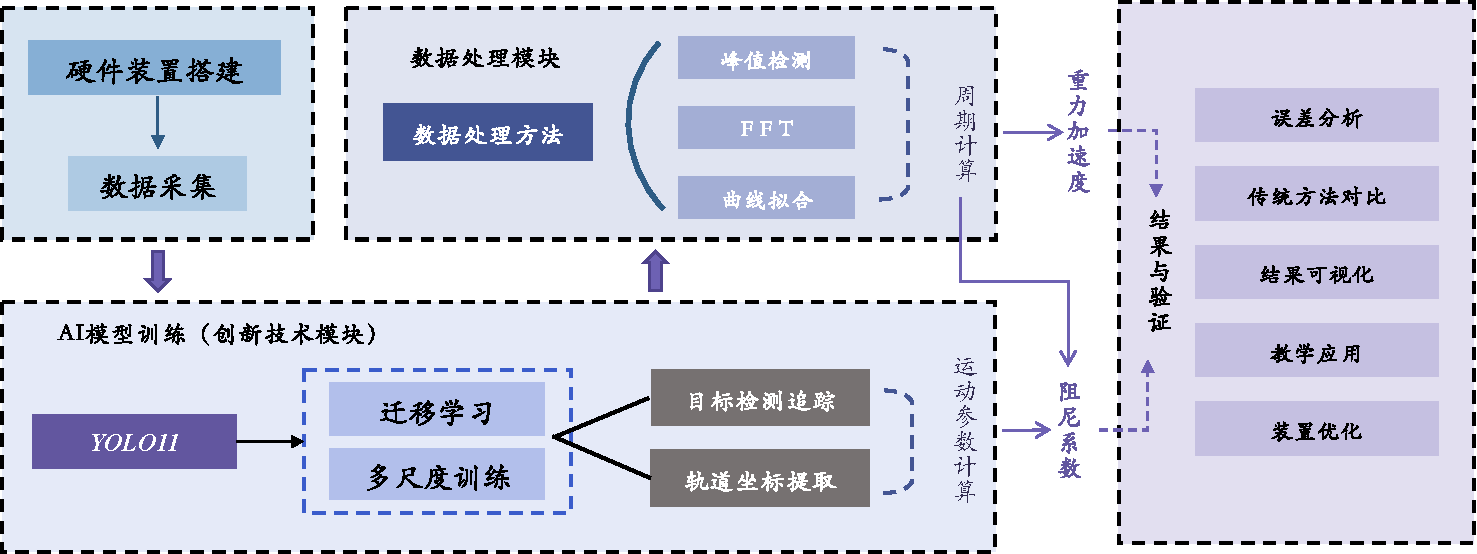
\includegraphics[width=1\textwidth]{figures/实验方案框架}
    \caption{实验方案框架}
    \label{实验方案框架}
\end{figure} 
\section{实验原理}
\subsection{物理实验原理}


 \begin{figure}[H]
    \centering
    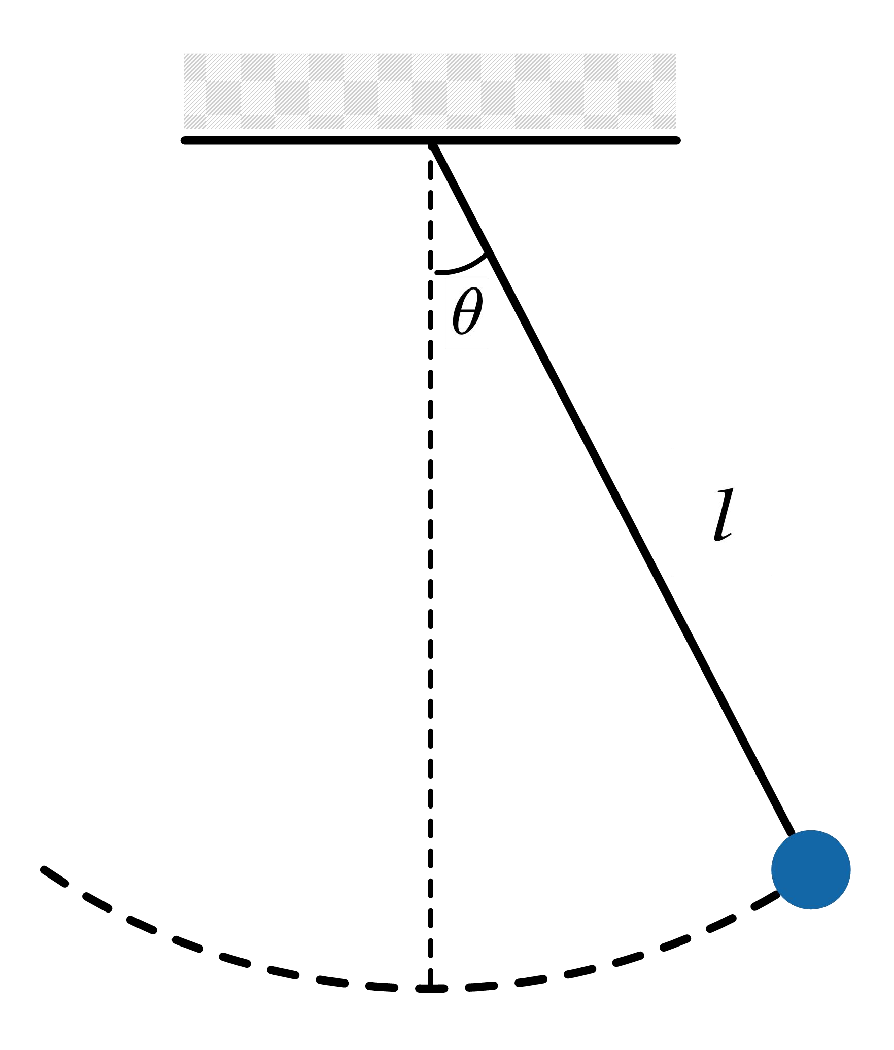
\includegraphics[width=0.2\textwidth]{figures/单摆}
    \caption{单摆模型示例图}
    \label{单摆}
 \end{figure}

 单摆是由一根无弹性的轻质细线和悬在此线一端的摆球组成。若将悬挂的摆球自平衡位置拉至一边,然后释放,摆球则在平衡位置左右作周期性的往返摆动,如图\ref{单摆}所示。

根据受力分析,单摆沿切线方向的回复力为:
\begin{equation}
f = -mg \sin \theta
\end{equation}
式中负号表示回复力方向与角位移 $\theta$ 相反。

根据牛顿第二定律,质点的加速度为 $a = \frac{f}{m}$,代入上式可得:
\begin{equation}
a = -g \sin \theta
\end{equation}

在单摆运动中,质点沿弧线运动,其角加速度可以表示为 $\alpha = \frac{d^2\theta}{dt^2}$,其中 $\alpha=\frac{a}{l}$ ,将其代入上式,得到:

\begin{equation}
\frac{d^2\theta}{dt^2} + \frac{g}{l} \sin \theta = 0
\end{equation}

令 $\omega^2 = \frac{g}{l}$,则方程可简化为:
\begin{equation}
\frac{d^2\theta}{dt^2} + \omega^2 \sin \theta = 0
\end{equation}

这便是单摆运动的微分方程,当$\theta$较小时(小于5°),$\sin \theta \approx \theta$,则方程可简化为:
\begin{equation}
\frac{d^2\theta}{dt^2} + \omega^2 \theta = 0
\end{equation}

\begin{TertiaryBox}[重力加速度测量原理]
根据微分方程理论,该方程的一般解为:
\begin{equation}
    \theta(t) = \theta_0 \cos(\omega t + \varphi_0)
\end{equation}

其中$\theta_0$为初始振幅,$\varphi_0$为初相位,$\omega$为角频率。将此解代入原微分方程式得:

\begin{equation}
  \omega = \sqrt{\frac{g}{l}}
\end{equation}

由振动周期$T$与角频率$\omega$的关系:$T = \frac{2\pi}{\omega}$,代入得:
\begin{equation}
T = \frac{2\pi}{\sqrt{\frac{g}{l}}} = 2\pi\sqrt{\frac{l}{g}}
\end{equation}
所以振动周期为:
\begin{equation}
T = 2\pi\sqrt{\frac{l}{g}}
\end{equation}
\end{TertiaryBox}

这表明单摆的振动周期只与摆长$l$和重力加速度$g$有关,与角振幅$\theta_0$无关,在实际测量中只需要测量出摆长$l$和周期$T$,就可以计算出重力加速度$g$。



\begin{TertiaryBox}[阻尼系数测量原理]
考虑空气阻尼的影响,运动方程修正为:
\begin{equation}
\frac{d^2\theta}{dt^2} + \frac{\beta}{m} \frac{d\theta}{dt} + \omega^2 \theta = 0
\end{equation}

其中 $\beta$ 为单摆系统的阻尼系数(单位:N$\cdot$s/m),$m$为摆球质量,其解为:
\begin{equation}
\theta(t) = \theta_0 e^{-\frac{\beta}{m} t} \cos(\omega t + \varphi_0)
\end{equation}
该解表示阻尼振动,在时间推移后角振幅逐渐衰减。
若测得初始角振幅 $\theta_0$ 和 $n$ 个周期后角振幅 $\theta_n$,则有:
\begin{equation}
\frac{\theta_0}{\theta_n} = \frac{\theta_0}{\theta_0 e^{-\frac{\beta}{m} nT}} = e^{\frac{\beta}{m} nT}
\end{equation}
取对数得阻尼系数:
\begin{equation}
\beta = \frac{m}{nT} \ln\left(\frac{\theta_0}{\theta_n}\right)
\end{equation}
\end{TertiaryBox}

在实际测量中,由于角振幅$\theta$难测量,可将其转化为测量摆球的水平振幅$A$,
根据$A = l\sin \theta,sin \theta \approx \theta$,可得$A = l\theta$,故:
$\beta = \frac{m}{nT} \ln\left(\frac{A_0}{A_n}\right)$,该式中$\frac{A_0}{A_n}$为振幅衰减比,像素振幅衰减比与实际振幅衰减比相同,故不需要将像素长度转换为实际长度。

以上结论均是在小角度近似下得出的,当$\theta$较大时,需要考虑非线性项的影响,摆球的周期$T$为与$\theta$有关,表达式\textsuperscript{\cite{DXWL200705004}}为:
\begin{equation}
T = 4 \sqrt{\frac{l}{g}} \int_{0}^{\frac{\pi}{2}} \frac{1}{\sqrt{1 - \sin^2 \frac{\alpha}{2} \sin^2 \varphi}} \, d\varphi
  = 2\pi\sqrt{\frac{l}{g}} \left( 1 + \sum_{n=1}^{\infty} \left( \frac{(2n-1)!!}{(2n)!!} \right)^2 \sin^{2n} \frac{\alpha}{2} \right)
\end{equation}


\subsection{AI技术原理}

YOLO 是目前为止最先进的目标检测方案之一\textsuperscript{\cite{7780460}},它能够在一幅图面中同时检测并分类出对象。

\subsubsection{YOLO 的神经网络结构}

YOLOv1\textsuperscript{\cite{DBLP:journals/corr/RedmonDGF15}}(2015 年)首次提出将图像划分为 S×S 网格(grid cell),每个网格预测B 个边界框(每个框包含位置坐标和置信度)和 C 个类别概率,最终输出张量维度为S×S×(B×5+C)。其网络结构分为两部分:

特征提取层:
采用 24 层卷积层(借鉴 GoogleNet 的 Inception 模块改进),通过 1×1 和 3×3 卷积组合提取多尺度特征,并交替使用最大池化层压缩特征图尺寸。

预测层:
包含 2 个全连接层,将特征图展平后直接回归边界框坐标和类别概率。输出层使用线性激活函数处理坐标,Sigmoid 函数处理置信度和类别概率。
 \begin{figure}[ht]
    \centering
    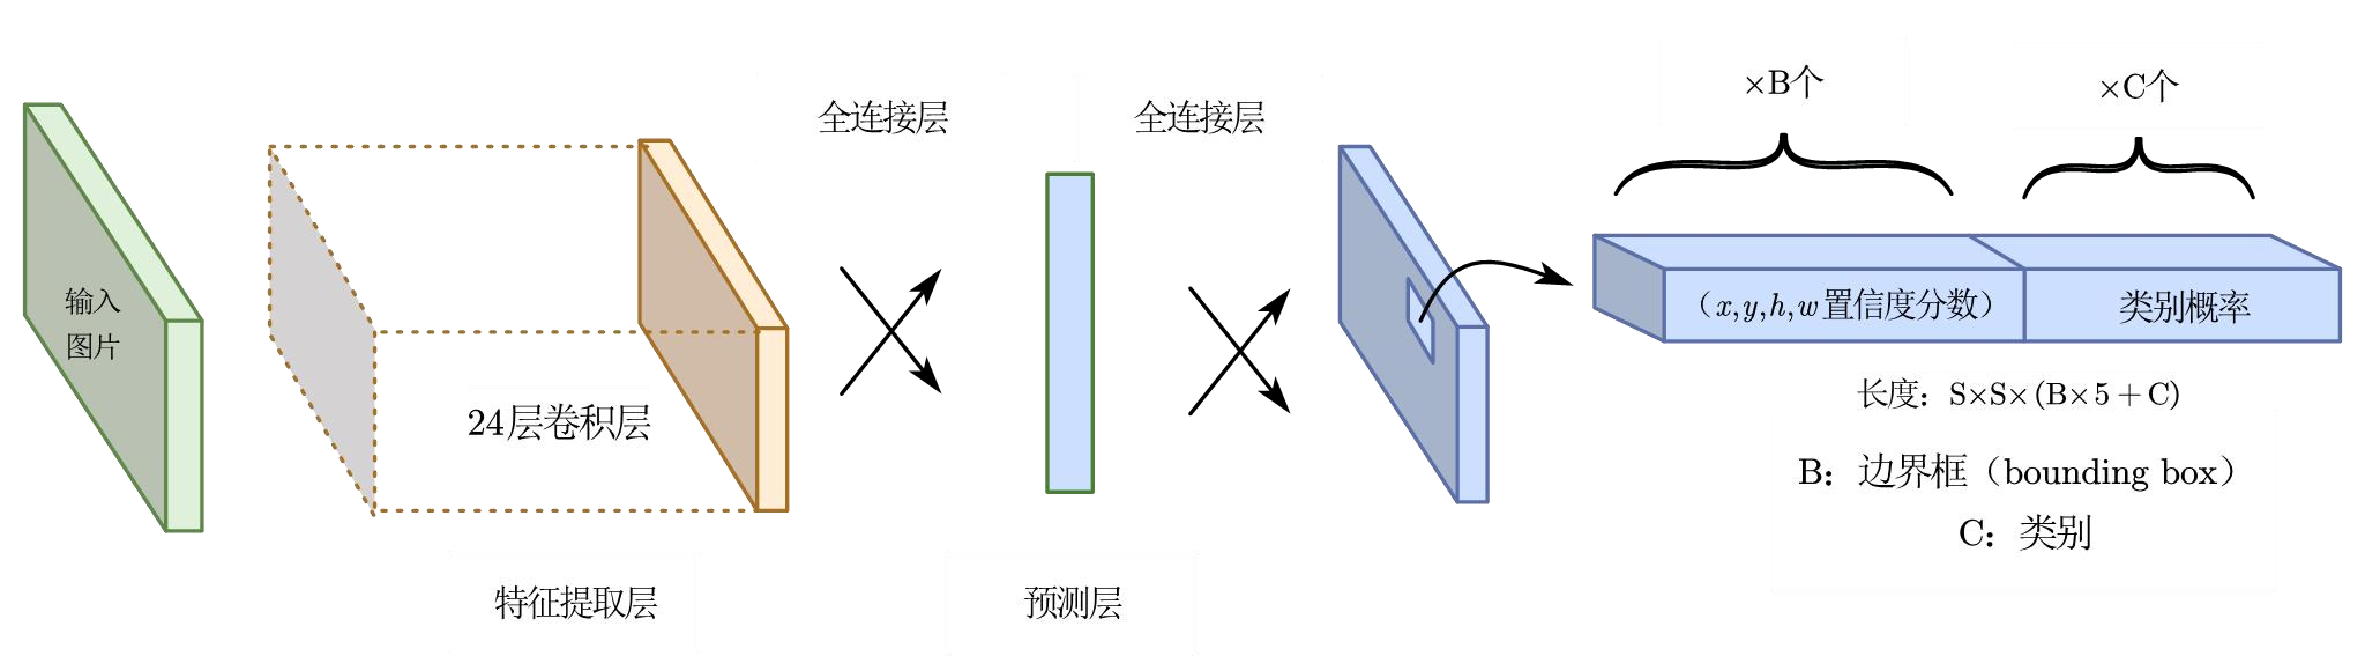
\includegraphics[width=0.8\textwidth]{figures/yolo神经网络结构.pdf}
    \caption{YOLO 的神经网络结构}
    \label{fig:yolo}
 \end{figure}

\subsubsection{YOLO 的损失函数}

基于均方误差(Sum of Squared Errors, SSE)的损失函数是机器学习中常用的损失函数,简单、容易优化 。同样 YOLO 网络中也是基于 SSE 构建来损失函数,如下:

\begin{equation}
loss = \sum_{i=0}^{S^2} coordError + iouError + classError
\end{equation}

由于以下两个原因,YOLO 团队对SSE进行了改进,以更好地平衡不同类型的误差:

\begin{enumerate}
  \item 在每个网格单元(grid cell)中,定位误差(localization error)、IOU 误差和分类误差(classification error)对总损失的影响存在显著差异,但 SSE 并未对这些误差进行区分处理。
  
  \item 图像中多数网格单元不包含目标物体,根据 YOLO 的设计,这些网格的 bounding box 的置信度(confidence)被设为 0。由于这些负样本数量庞大,其在梯度更新中的总贡献反而可能超过了包含目标的正样本,导致模型训练不稳定。
\end{enumerate}

为解决上述问题,YOLO 引入了一个改进的损失函数\textsuperscript{\cite{DZYX202210040}},在整体上实现了对定位误差、IOU 误差和分类误差的平衡。该损失函数的形式如下:

\begin{align}
\text{Loss Function} = & \lambda_{\text{coord}} \sum_{i=0}^{S^2} \sum_{j=0}^{B} \mathbf{1}_{ij}^{\text{obj}} \big[ (x_i - \hat{x}_i)^2 + (y_i - \hat{y}_i)^2 \big] \nonumber 
 + \lambda_{\text{coord}} \sum_{i=0}^{S^2} \sum_{j=0}^{B} \mathbf{1}_{ij}^{\text{obj}} \big[ (\sqrt{w_i} - \sqrt{\hat{w}_i})^2 \\
 &+ (\sqrt{h_i} - \sqrt{\hat{h}_i})^2 \big] \nonumber 
  + \sum_{i=0}^{S^2} \sum_{j=0}^{B} \mathbf{1}_{ij}^{\text{obj}} (C_i - \hat{C}_i)^2 \nonumber 
   + \lambda_{\text{noobj}} \sum_{i=0}^{S^2} \sum_{j=0}^{B} \mathbf{1}_{ij}^{\text{noobj}} (C_i - \hat{C}_i)^2 \nonumber \\
  &+ \sum_{i=0}^{S^2} \mathbf{1}_{i}^{\text{obj}} \sum_{C \in \text{classes}} (p_i(C) - \hat{p}_i(C))^2
\end{align}


式中 $x_i$ 和 $y_i$ 为预测目标的 $x$ 和 $y$ 轴坐标,$\hat{x}_i$ 和 $\hat{y}_i$ 为实际目标的 $x$ 和 $y$ 轴坐标;$w_i$ 和 $h_i$ 为预测目标的宽和高,$\hat{w}_i$ 和 $\hat{h}_i$ 为实际目标的宽和高;$C_i$ 为预测目标的类别,$\hat{C}_i$ 为实际目标的类别。第四项是对背景的置信度的预测。第五项是对物体类别的预测 $P_r(Class_i|Object)$,$p_i(C)$ 为预测目标的置信度,$\hat{p}_i(C)$ 为实际目标的置信度;$\lambda_{coord}$ 和$\lambda_{noobj}$是为了平衡各项 Loss 的比重所设定的权值,分别为 5 和 0.5。S 为每一个网格单元,B 为每一个边界框,obj为含有目标,noobj 为不含目标。

\begin{figure}[ht]
    \centering
    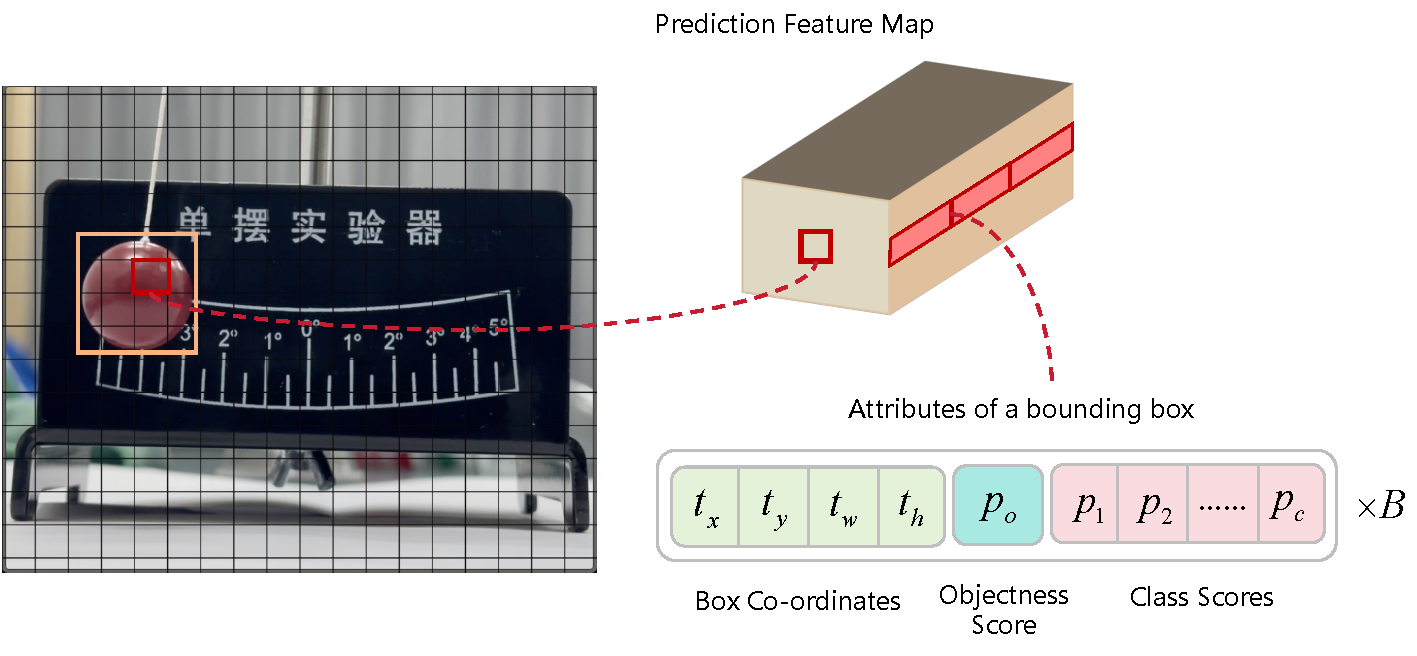
\includegraphics[width=0.9\textwidth]{figures/图片在网格中的处理.pdf}
    \caption{图片在网格中的处理过程}
    \label{fig:grid_process}
\end{figure}


\subsubsection{基于YOLO的摆球识别}
本文提出的基于深度学习 YOLO 的摆球识别方法能够定位视频中的摆球并返回其标。不同于基于区域预测的目标检测算法(Faster RCNN),YOLO 通过单个卷积神经网络检测整个图像回归目标的类别和位置,为了让卷积遍历整幅图像之后能够得到固定格式的预测大小,首先将图像调整为固定大小的尺寸640×640,再分成S×S 的非重叠的网格单元,然后每个单元负责检测出该单元可能拥有的 B 个边界框及其置信度,具体包含 5 个预测参数:x,y,w,h 和置信度。(x,y)代表目标的坐标,(w,h)代表目标外包矩形的宽度和高度,置信度用来通过阈值对预测结果进行取舍。 
\section{实验装置设计}
本章节主要介绍单摆实验装置的设计,包括单摆实验装置的设计、AI辅助系统的设计以及实验装置的系统误差分析。
\subsection{单摆实验装置设计}

本实验采用精密单摆装置,其主要构成包括:线长调节轮盘、高精度摆线、金属支撑杆、稳固底座、精密刻度盘及标准带孔摆球。装置设计遵循物理实验精确性和操作便捷性原则。

线长调节轮盘内部集成长度约1米的高强度细线,通过精密啮合机构实现摆线长度的连续可调与精确控制。根据单摆理论,摆线的有效长度被定义为线段长度与悬挂钢球半径之和,这一参数对实验测量结果具有决定性影响。

支撑系统由直径7.5 mm的高强度金属杆构成,提供足够的刚性支撑,有效减小实验过程中的系统振动误差。底座及刻度盘采用一体化加厚设计,显著提升整体结构稳定性,同时刻度盘上精确标记的角度刻度使摆动初始角度的设定和读数更为精确,满足定量实验需求。

实验用摆球包含多种材质和规格,具体包括:带孔钢球(直径约19 mm,质量约27 g,1颗)、带孔钢球(直径约13 mm,质量约6.5 g,2颗)、带孔塑料球(直径约27 mm,质量约9 g,1颗)、带孔塑料球(直径约19 mm,质量约4 g,1颗)。所有摆球均为中心穿孔设计,便于摆线安装与固定,确保摆动过程中质量分布的均匀性。

该装置整体高度为41 cm,底座尺寸为11.5 cm×9 cm,净重约570 g。整体结构紧凑、参数稳定、操作简便,适用于教学实验及科研工作中重力加速度测量、简谐运动分析等相关物理实验。
\begin{figure}[H]
    \centering
    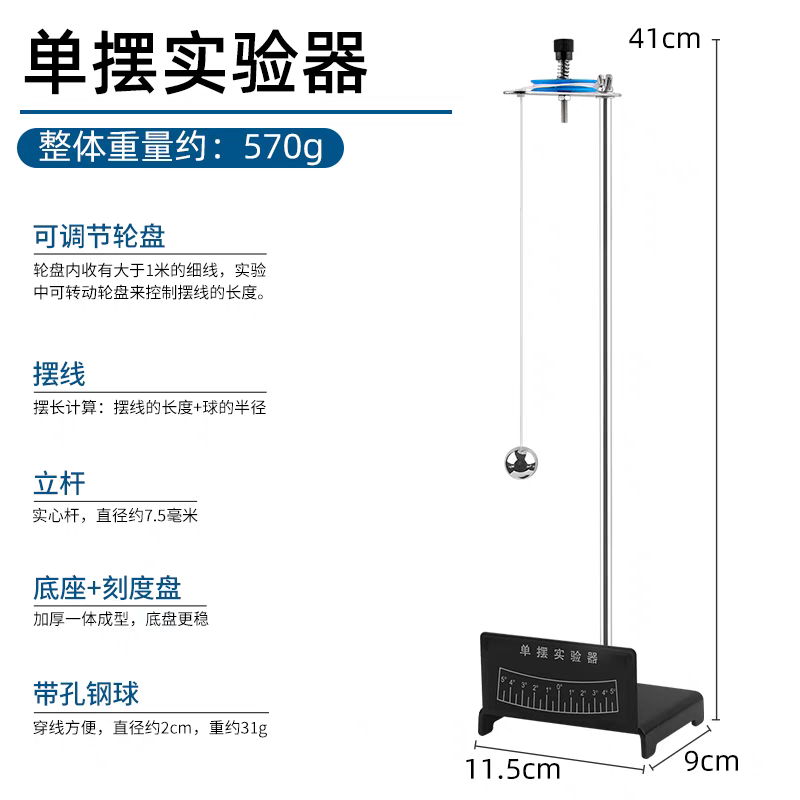
\includegraphics[width=0.45\textwidth]{figures/单摆实验装置1.jpg}
    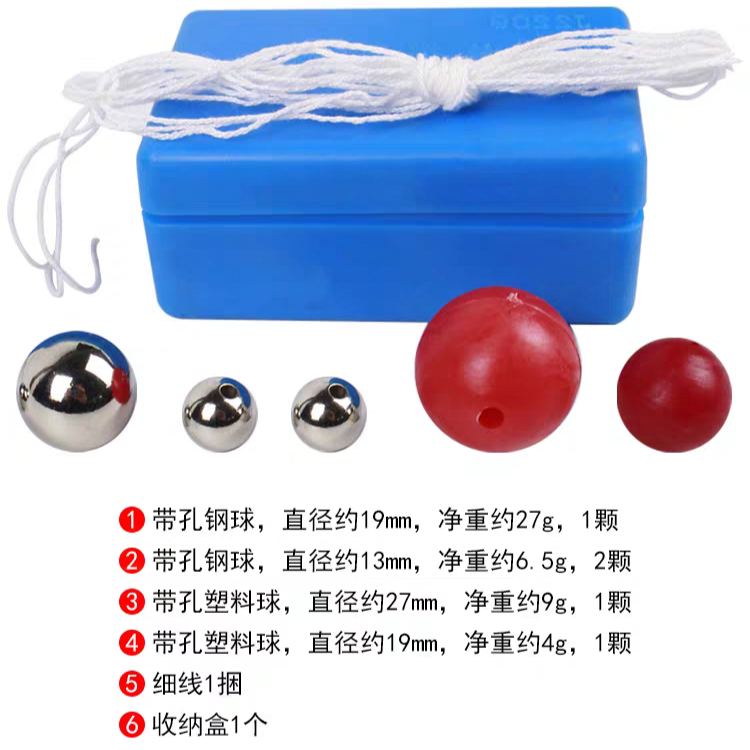
\includegraphics[width=0.45\textwidth]{figures/单摆实验装置2.jpg}
    \caption{单摆实验装置}
    \label{fig:pendulum_device}
\end{figure}

\subsection{AI辅助系统设计}

针对上文的单摆实验装置,本项目设计了基于深度学习的单摆实验AI辅助系统,旨在通过计算机视觉技术实现单摆运动的\textbf{自动跟踪、数据采集与分析,提高物理实验的精确性}。该系统采用YOLO目标检测算法精确识别并追踪摆球位置,通过多种数据分析方法计算单摆周期与重力加速度,实现了从视频输入到物理参数计算的完整自动化流程。系统的实现包含数据集采集与处理、模型训练与评估以及软件实现三大部分,整套系统将AI技术与物理实验有机结合,有效解决了传统人工观测耗时费力且精度有限的问题。

\subsubsection{数据集的采集与处理}

为确保模型的鲁棒性,本团队在多种环境条件下采集装置的训练数据集。数据集由100张高质量图像组成,按照4:1的比例划分为训练集(80张)和验证集(20张),以确保模型具有良好的泛化能力,数据标注采用labelImg工具进行人工标注,标注格式遵循YOLO数据集标准规范。每个标注包含以下信息:
\begin{itemize}
    \item 类别ID(class\_id):标识目标类别;
    \item 中心点坐标(x\_center, y\_center):目标框中心点位置;
    \item 边界框尺寸(width, height):目标框的宽度和高度;
\end{itemize}

所有坐标值均归一化到[0,1]区间,以确保数据的一致性和可比性。标注完成后,数据按照标准目录结构进行组织,如图\ref{fig:dataset_structure}所示,为后续模型训练做好准备。

\begin{figure}[H]
    \centering
    \subfigure[数据集目录结构]{
        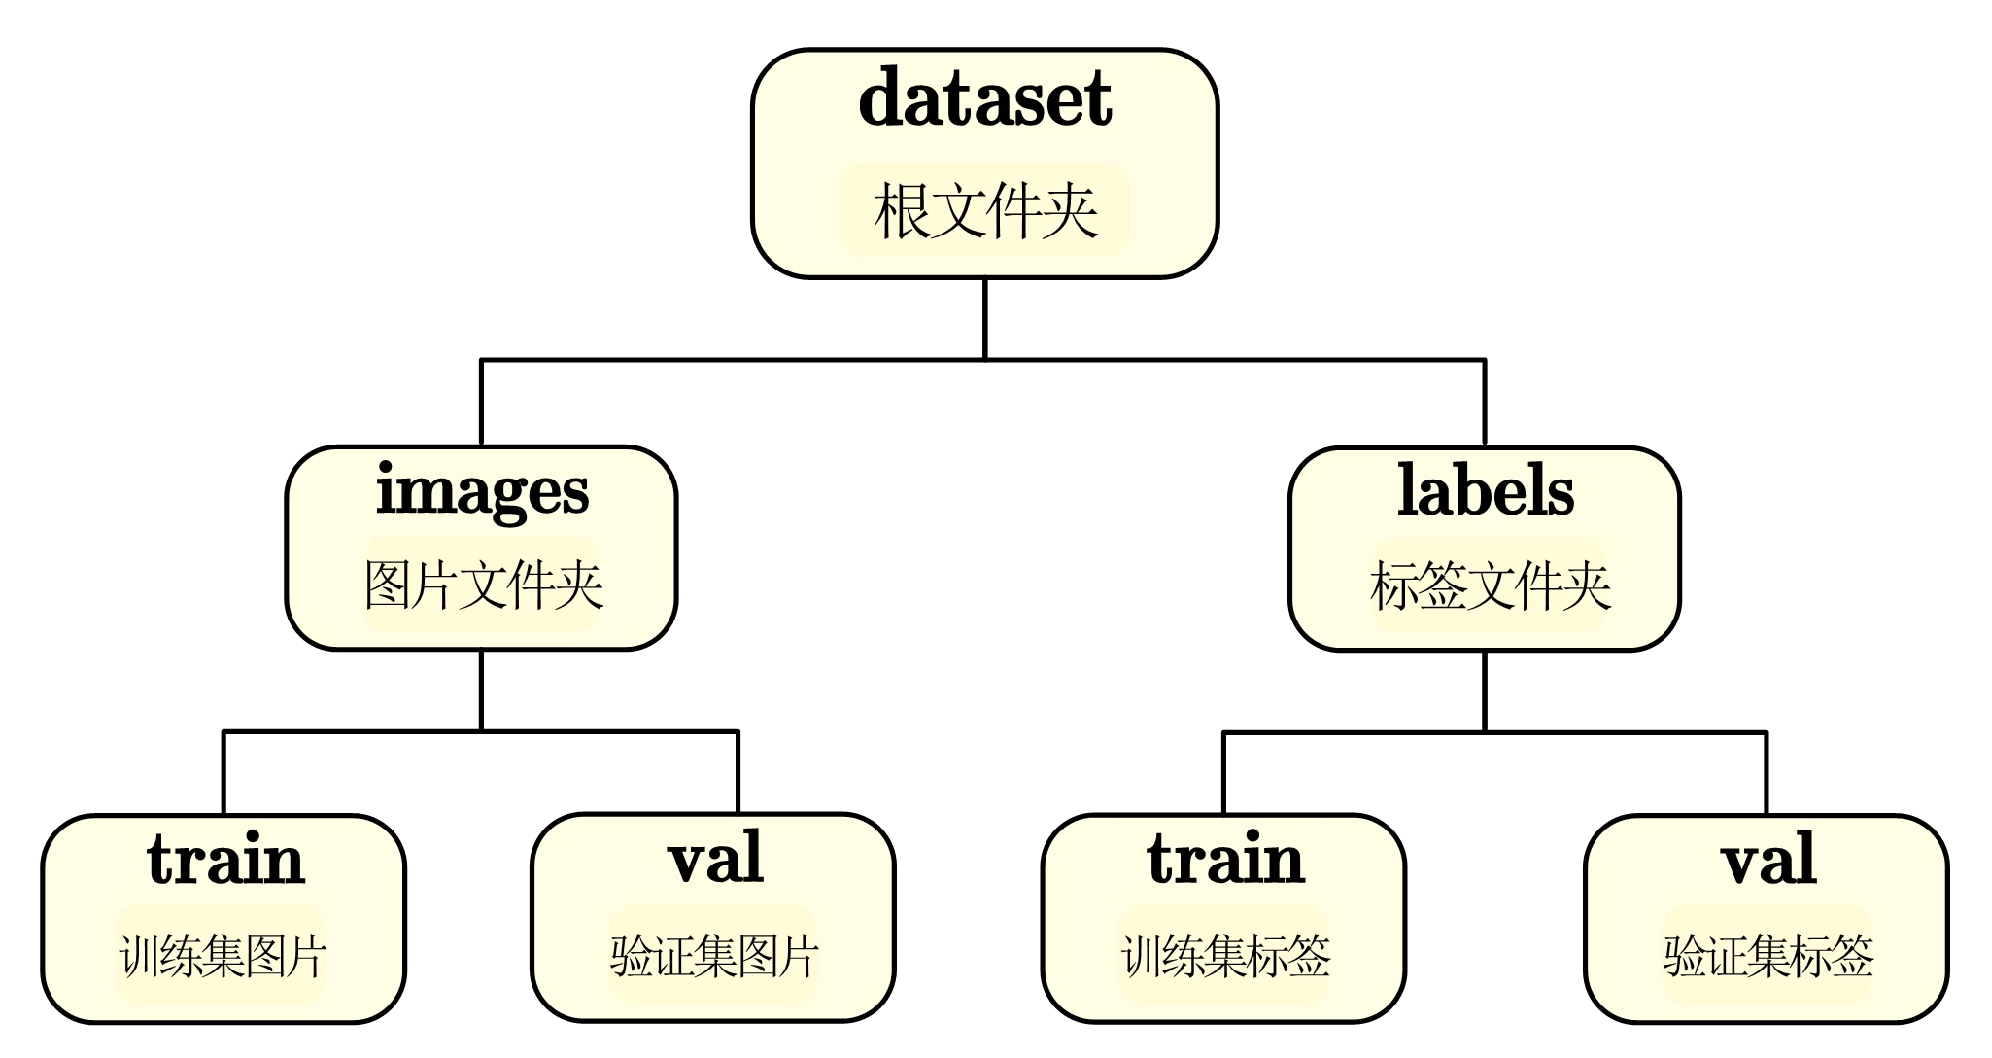
\includegraphics[width=0.48\textwidth]{figures/数据集结构图}
        \label{fig:dataset_structure}
    }
    \hfill
    \subfigure[labelImg软件标注界面]{
        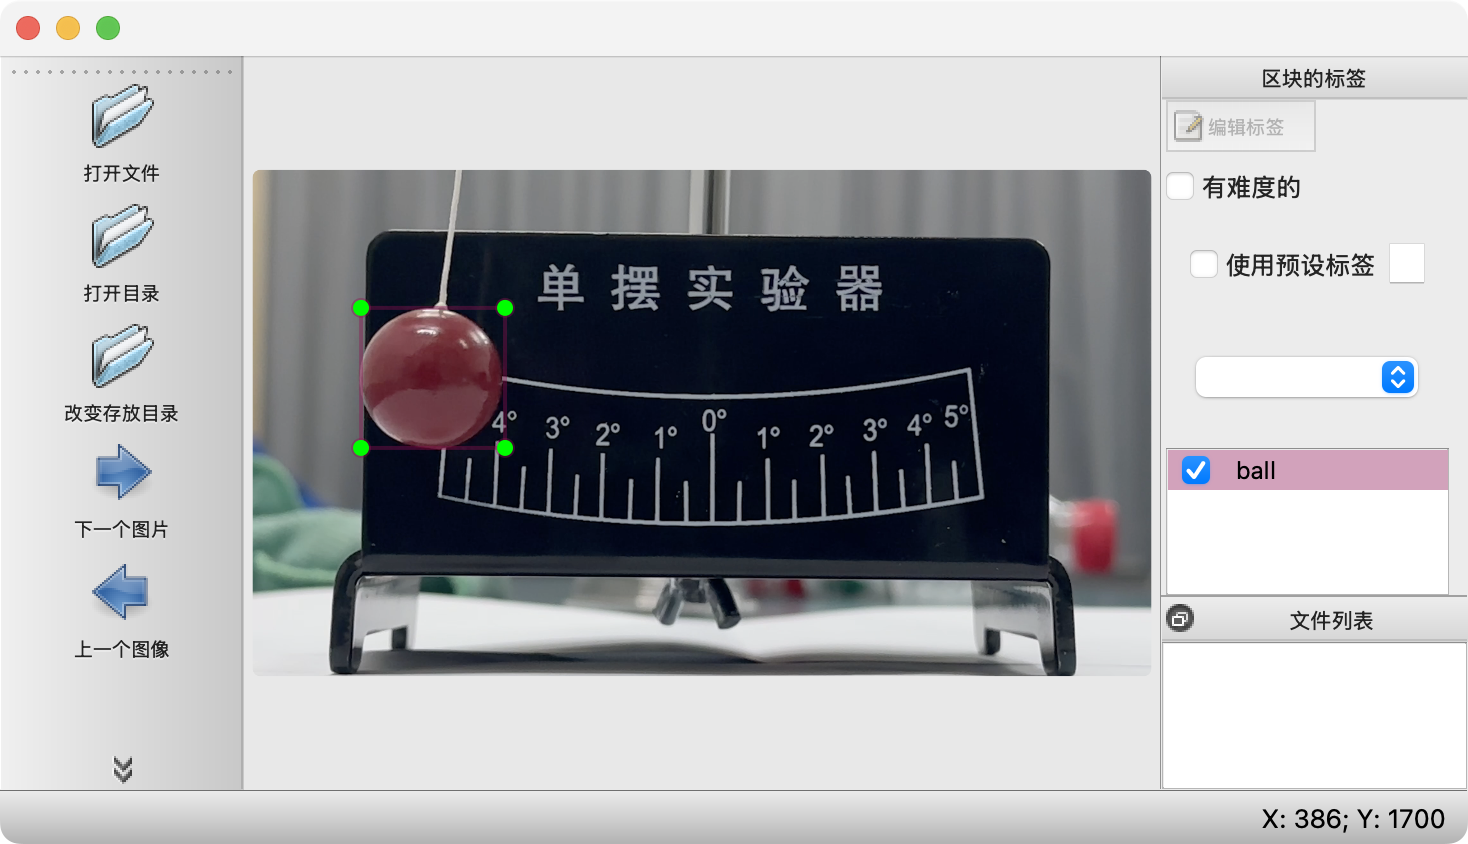
\includegraphics[width=0.48\textwidth]{figures/标注1.png}
        \label{fig:labelImg}
    }
    \caption{数据集标注与数据集目录结构}
    \label{fig:dataset}
\end{figure}

\subsubsection{模型的训练与评估}
本团队将epoch(训练轮数)设置为100,并开启多尺度训练增强训练的效果,最终到得到了最佳训练结果,保存为best.pt的权重文件。其 Loss 变化图如图\ref{fig:loss_change}所示。
可以看出,模型在前50次迭代中迅速拟合,后50次迭代后渐渐稳定,只有稍许震荡,说明训练效果较好。本团队另外拍摄了一段实验装置的视频,使用训练后的模型进行检测,\textbf{检测框全程稳定跟踪,置信度达到0.9以上},如图\ref{fig:video_test}所示,模型检测能力较好,可以用于后续的测量实验。
\begin{figure}[H]
    \centering
    \subfigure[Loss变化图]{ 
        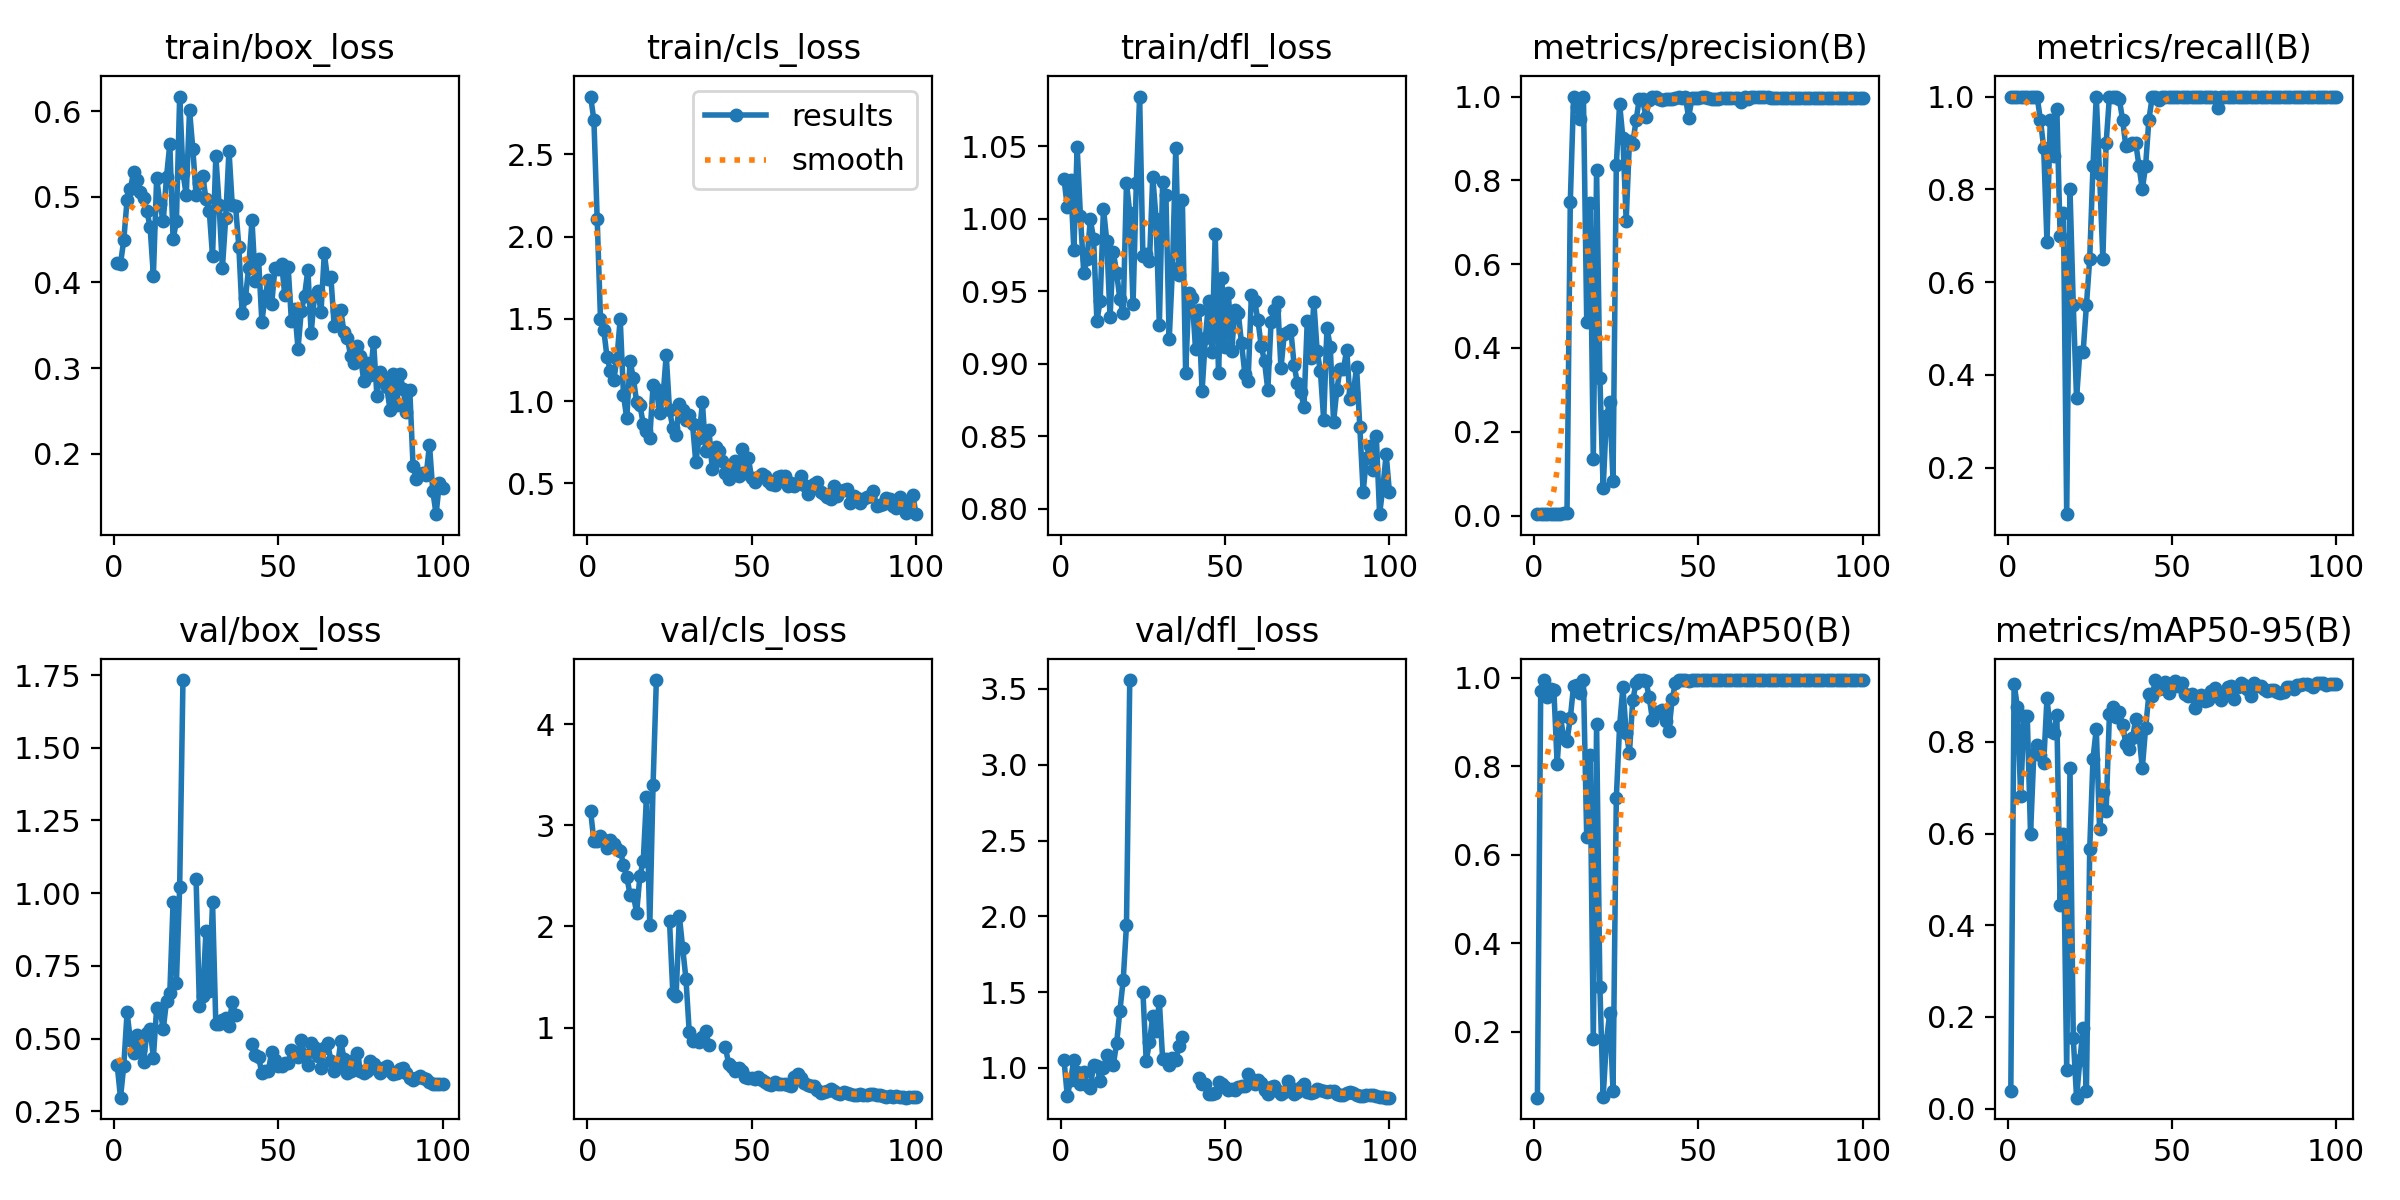
\includegraphics[width=0.55\textwidth]{figures/训练结果.png}
        \label{fig:loss_change} 
    }
    \subfigure[测试视频的检测结果]{
        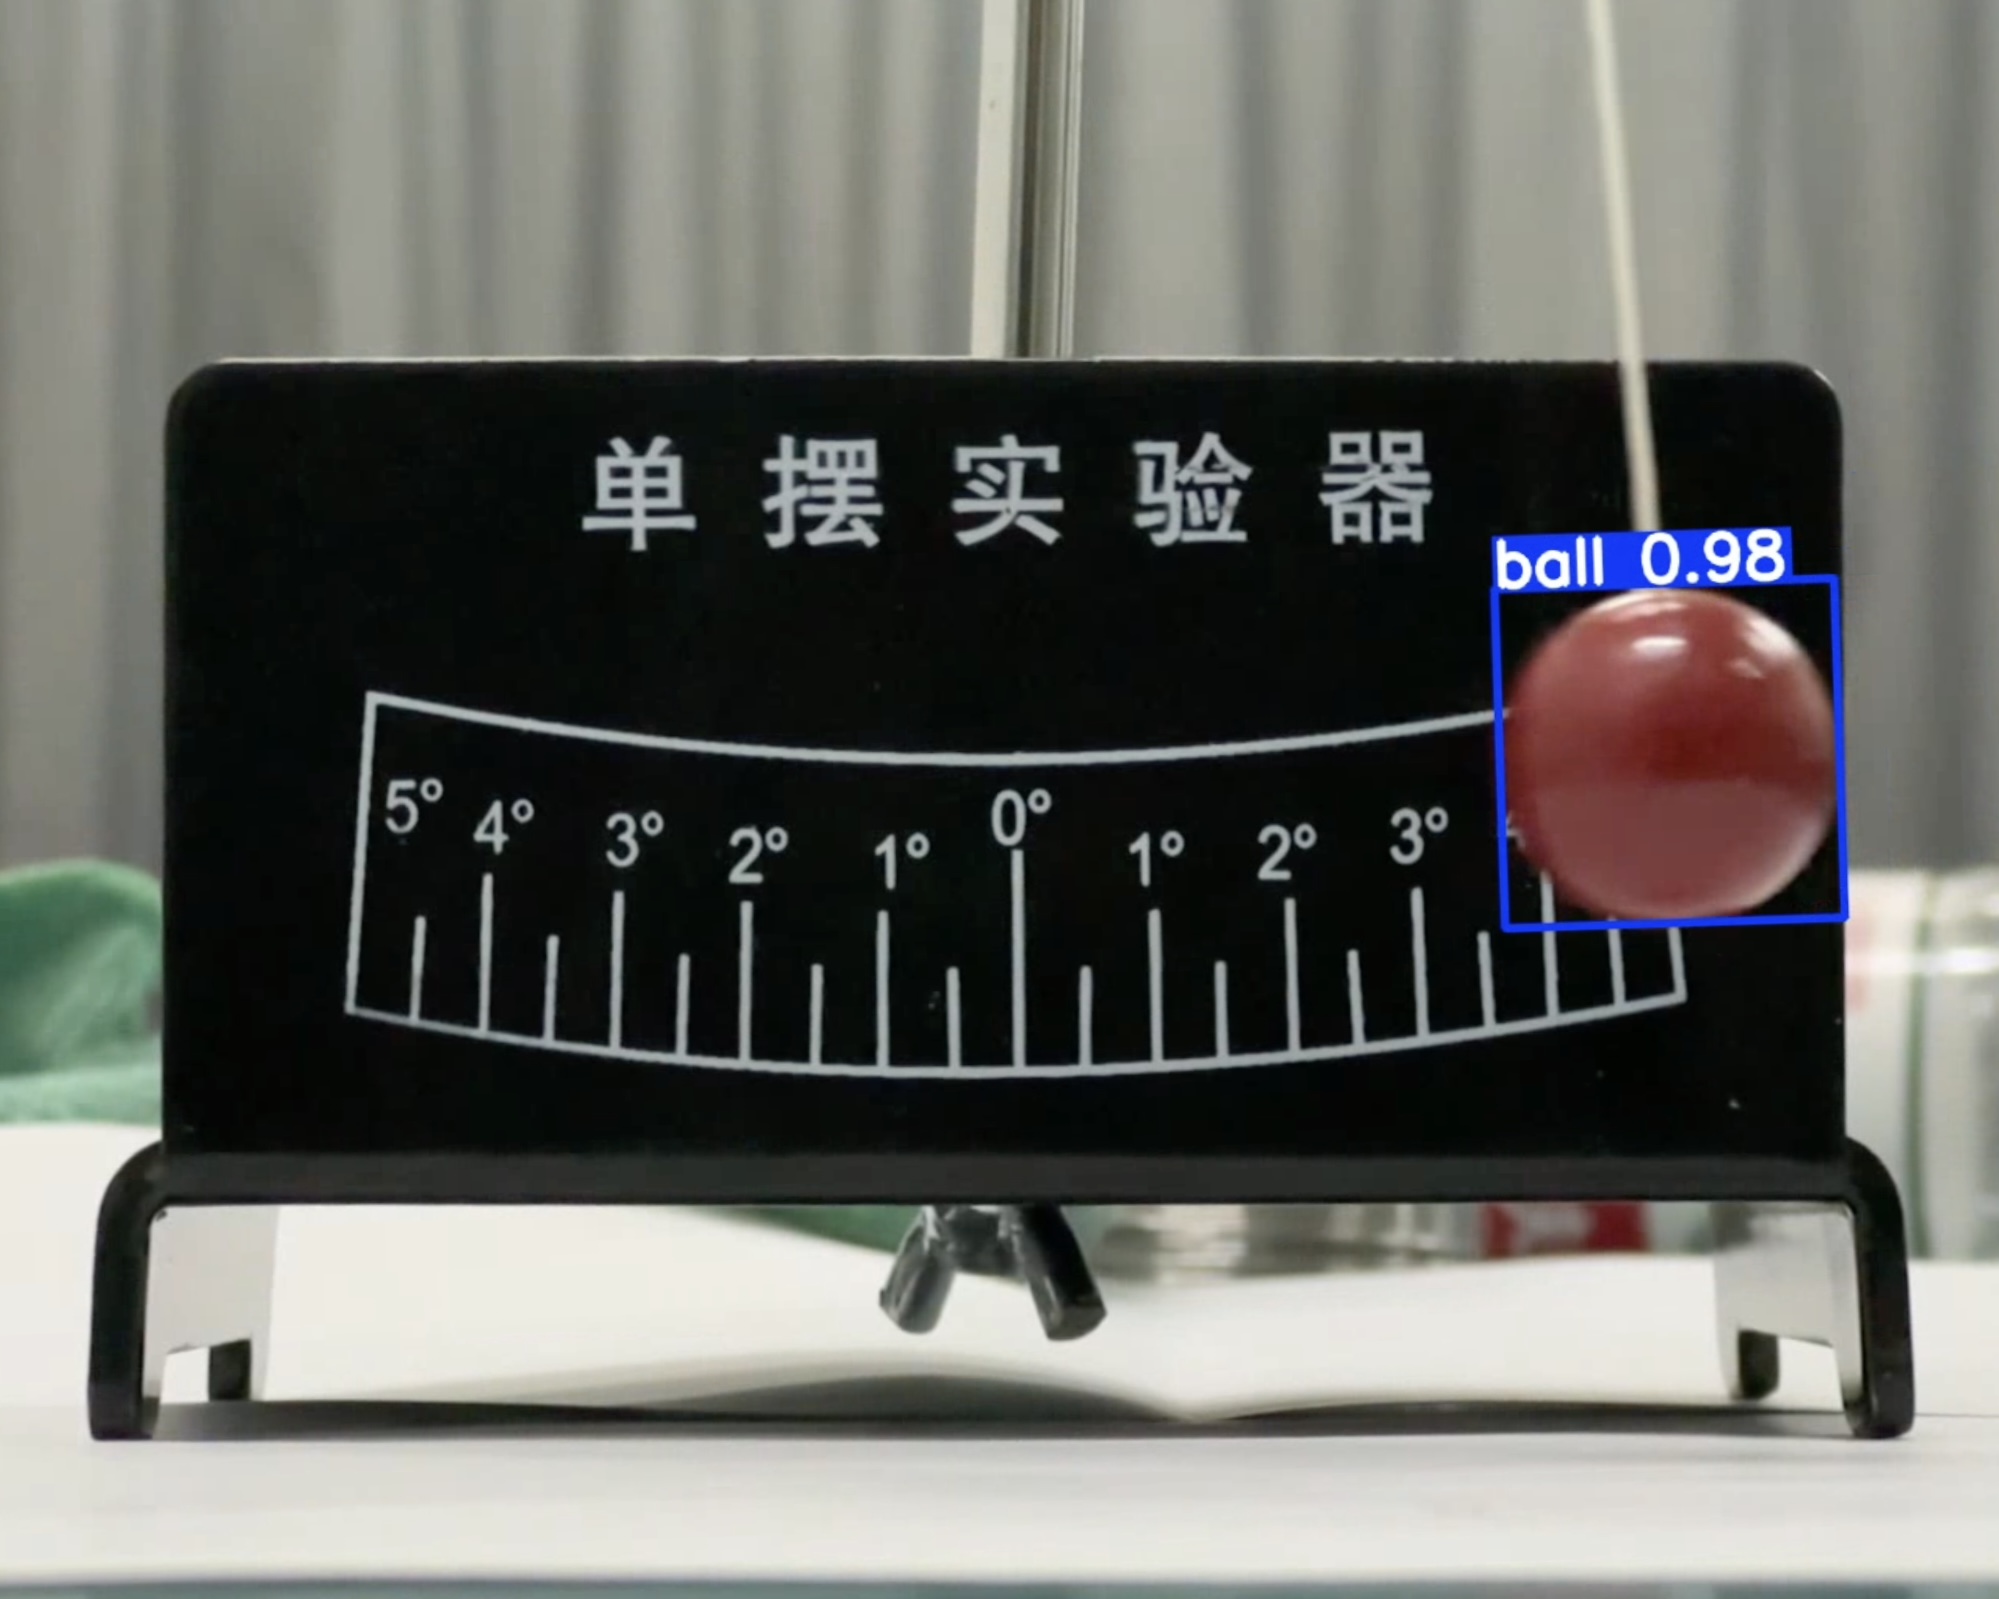
\includegraphics[width=0.35\textwidth]{figures/摆球识别效果2}
        \label{fig:video_test}
    }
    \caption{模型训练结果与识别效果}
    \label{fig:test_result}
\end{figure}

\subsubsection{软件设计}

在训练出能够精准识别摆球的AI模型后,本团队开发了一款集成相关功能的软件,便于其在实验中应用。本软件使用Python编写,依赖于多个第三方库,如PySide6(用于构建图形用户界面)、OpenCV(用于视频和图像处理)、ultralytics(包含YOLO模型,用于目标检测)、numpy、pandas、scipy(用于数值计算)以及matplotlib(用于绘图和数据可视化)。软件采用\textbf{模块化设计,各模块功能分离,便于维护和扩展},其结构图如图\ref{fig:software_structure}所示,包含三个主要模块:\texttt{gui.py}、\texttt{tracker.py} 和 \texttt{analyzer.py},源代码见附录\ref{app:software_code}。
下面将详细介绍每个模块的功能。

\begin{figure}[H]
    \centering
    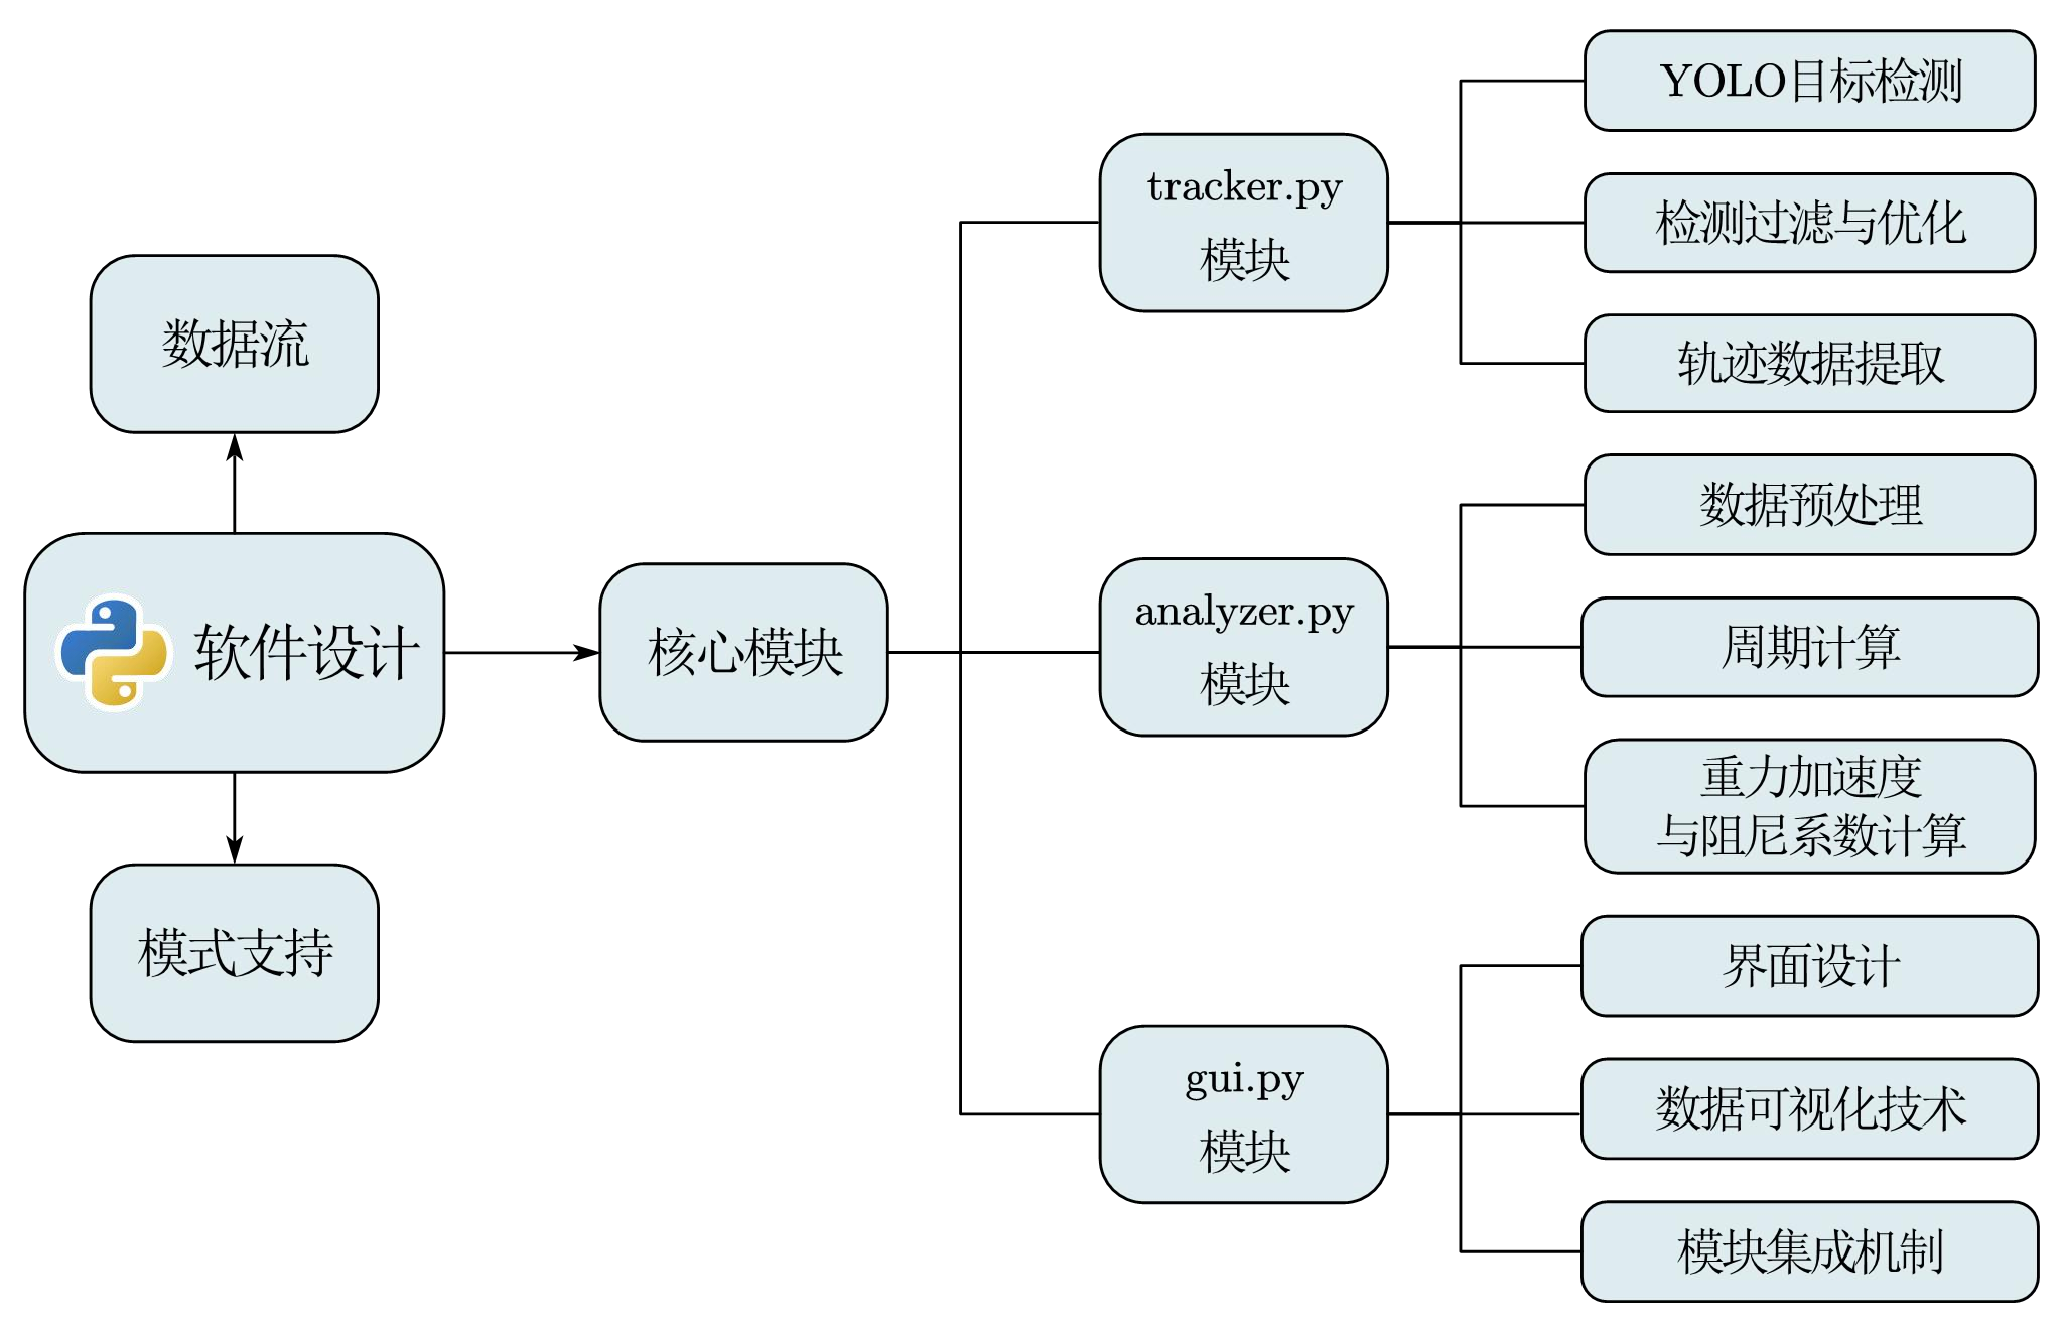
\includegraphics[width=0.7\textwidth]{figures/软件结构图.pdf}
    \caption{软件结构图}
    \label{fig:software_structure}
\end{figure}

\textbf{tracker.py模块},该模块负责目标检测和视频数据处理,实现小球的自动追踪与位置记录,完成\textbf{物理现象的观察}。其核心算法包括:
\begin{enumerate}
\item YOLO目标检测:系统运用YOLO深度学习模型实现单摆小球的快速识别。YOLO模型将图像分割为网格,每个网格预测边界框和类别概率,最终通过非极大值抑制(NMS)算法过滤重叠边界框,实现物体定位。相比传统计算机视觉方法,YOLO能够适应不同光照条件和背景干扰,提高小球定位精度。
    
\item 检测过滤与优化:系统实现了基于时间连续性的检测过滤机制,通过比较连续帧之间的边界框大小变化,筛除异常检测结果。该算法使用滑动窗口存储历史检测框大小,并通过中位数过滤实现对摆球运动轨迹的平滑跟踪,有效解决了传统视频处理中因光照变化、运动模糊等因素导致的识别不稳定问题。
    
\item 轨迹数据提取:系统从YOLO检测结果中提取小球中心坐标,并将其与实验时间戳关联,生成时间-位置数据序列。这种方法实现了小球运动过程的高精度记录,相较于传统的手动计时和目测方法,大幅提高了数据采集的精度和效率。

\end{enumerate}
\begin{figure}[H]
    \centering
    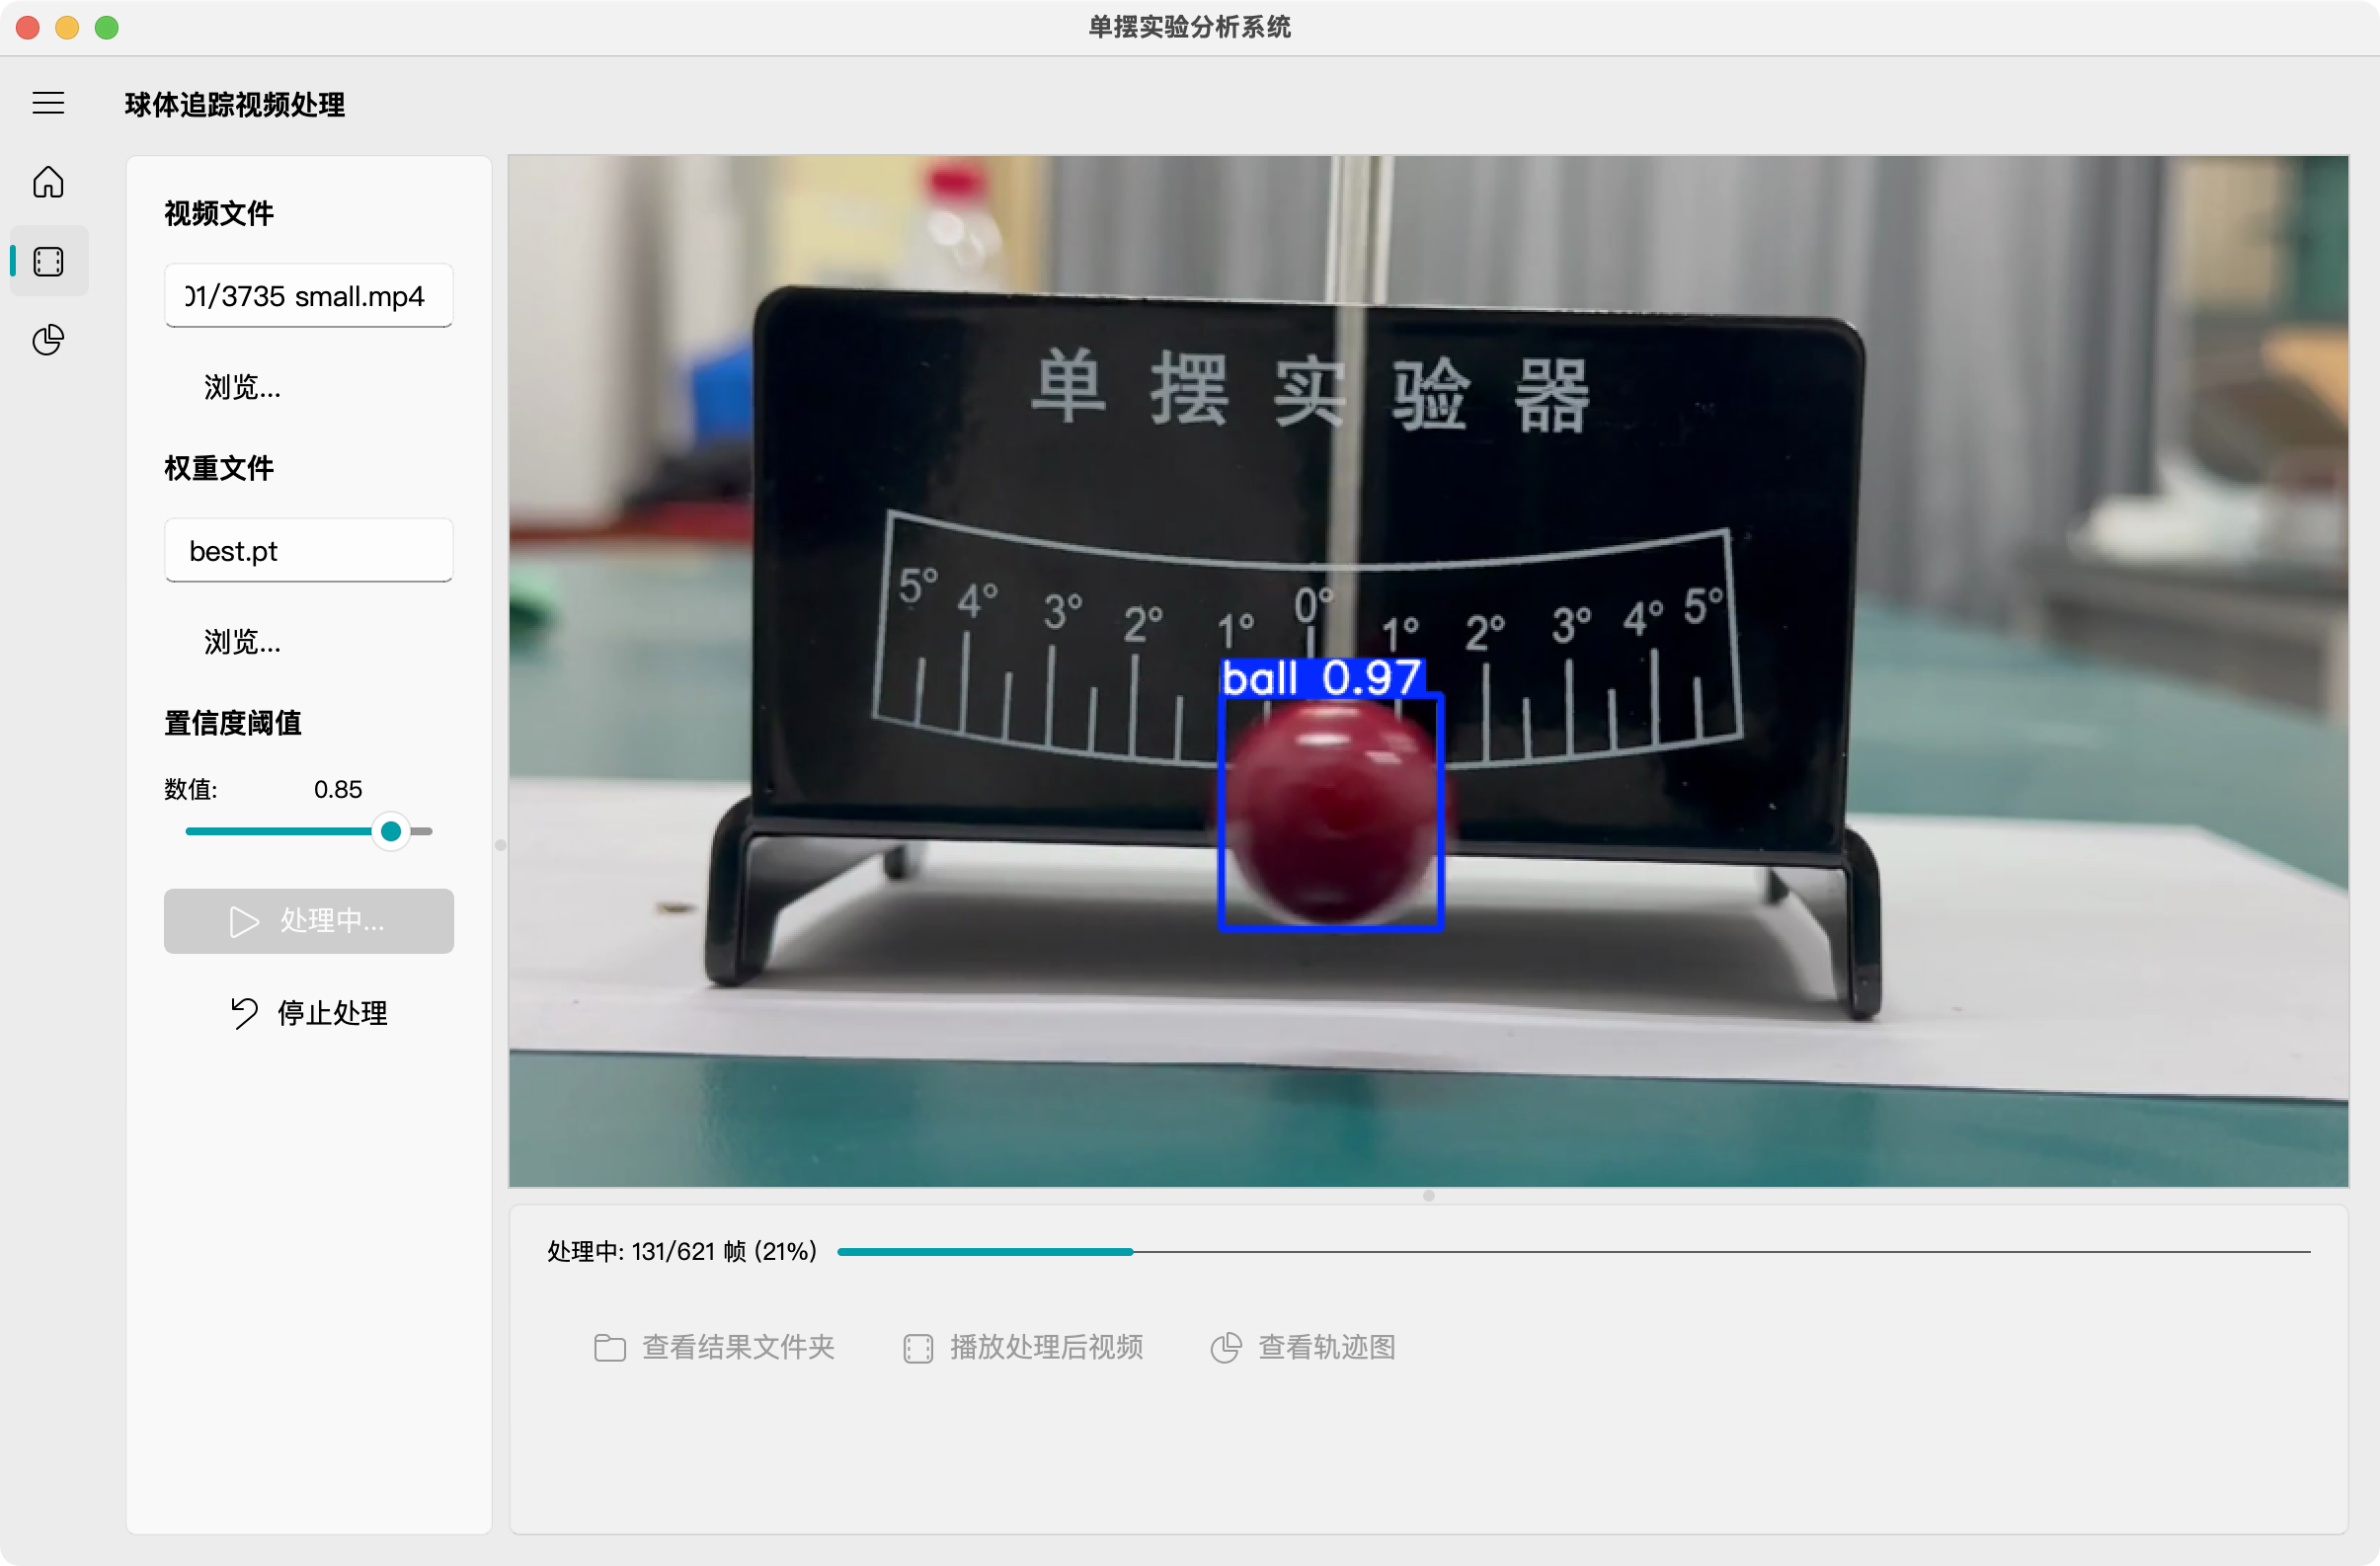
\includegraphics[width=0.5\textwidth]{figures/视频处理界面.png}
    \caption{视频处理界面}
    \label{fig:video_processing}
\end{figure}

\textbf{analyzer.py模块},该模块负责对轨迹数据进行物理分析,实现周期测量、重力加速度和阻尼系数等\textbf{物理参数的计算}。核心算法包括:
\begin{enumerate}
\item 数据预处理:系统采用Savitzky-Golay滤波器进行数据平滑,该滤波器通过局部多项式最小二乘拟合实现信号降噪。其核心思想是在时域上对数据点应用移动窗口,在每个窗口内使用多项式拟合局部数据,进而获得滤波点。与简单移动平均不同,该方法能够较好地保留信号的高频特征(如峰值和快速变化),同时有效抑制噪声,特别适合处理周期性运动数据。
    
\item 周期计算方法:系统提供三种互补的周期分析方法,实现高精度周期测量:
    \begin{enumerate}[label=\alph*.]
        \item 快速傅里叶变换(Fast Fourier Transform,FFT)分析法\textsuperscript{\cite{9787115284846001}}:该方法首先将时域信号转换到频域,通过分析频谱中的能量分布,识别出主频率。FFT分析特别适用于包含多频率成分的信号,但对于时间序列有限的情况,可能存在频率分辨率的限制。为提高精度,系统采用了汉宁窗(Hanning window)预处理信号并进行零填充(zero-padding),增强频谱分析的频率分辨率;
        
        \item 峰值检测法:该方法直接在时域上工作,通过识别位移-时间曲线中的局部极大值点(峰值),计算相邻峰值间的时间差作为周期估计。系统通过设置最小峰值距离和显著性阈值(prominence)参数,提高了峰值检测的准确性。该方法直观且计算效率高,但对噪声较为敏感;
        
        \item 曲线拟合法:该方法基于单摆的理论模型,通过最小二乘法将简谐运动方程 $x(t) = A\sin(\omega t + \phi) + C$ 拟合到实验数据。该方法利用整个数据集信息,对噪声具有较强的鲁棒性,且能同时提取振幅、频率和相位等多个参数,但计算复杂度较高,且依赖于初始参数估计。
    \end{enumerate}
    
  
\item 重力加速度计算:根据单摆理论,周期$T$与摆长$l$和重力加速度$g$的关系为$T = 2\pi\sqrt{l/g}$。系统基于此公式,结合周期测量结果,计算得到重力加速度$g = 4\pi^2l/T^2$。为提高大摆角条件下的计算精度,系统还实现了非线性周期修正,考虑摆角$\theta$的影响:$T = T_0(1 + \frac{1}{16}\theta^2 + \frac{11}{3072}\theta^4 + ...)$,其中$T_0$为小摆角条件下的理论周期。
    
\item 阻尼系数计算:系统采用对数衰减法计算阻尼系数。
    在单摆系统中,空气阻力产生的阻尼使振动振幅随时间呈指数衰减:$A(t) = A_0e^{-\frac{\beta}{m} t}$,其中$\beta$为阻尼系数,$m$为摆球质量。
    根据实验数据,系统首先提取振动峰值点,获得一系列时间-振幅数据对$(t_i, A_i)$,然后基于公式$\beta = \frac{m}{nT}\ln\frac{A_0}{A_n}$计算阻尼系数,
    其中$n$为周期数,$T$为平均周期,$A_0$为初始振幅,$A_n$为$n$个周期后的振幅。系统还计算了相关参数:固有频率$\omega_0 = 2\pi/T$、
    品质因数$Q = \omega_0/(\beta/m)$及衰减时间常数$\tau = m/\beta$。为直观展示衰减规律,系统对振幅取对数后进行线性拟合,斜率即为阻尼系数与质量比值$\beta/m$的相反数,
    通过可视化对比理论与实测的衰减曲线,验证了阻尼模型的有效性。该方法能够有效表征空气阻力对单摆运动的影响,为阻尼振动研究提供定量分析手段。
\end{enumerate}

\begin{figure}[H]
    \centering
    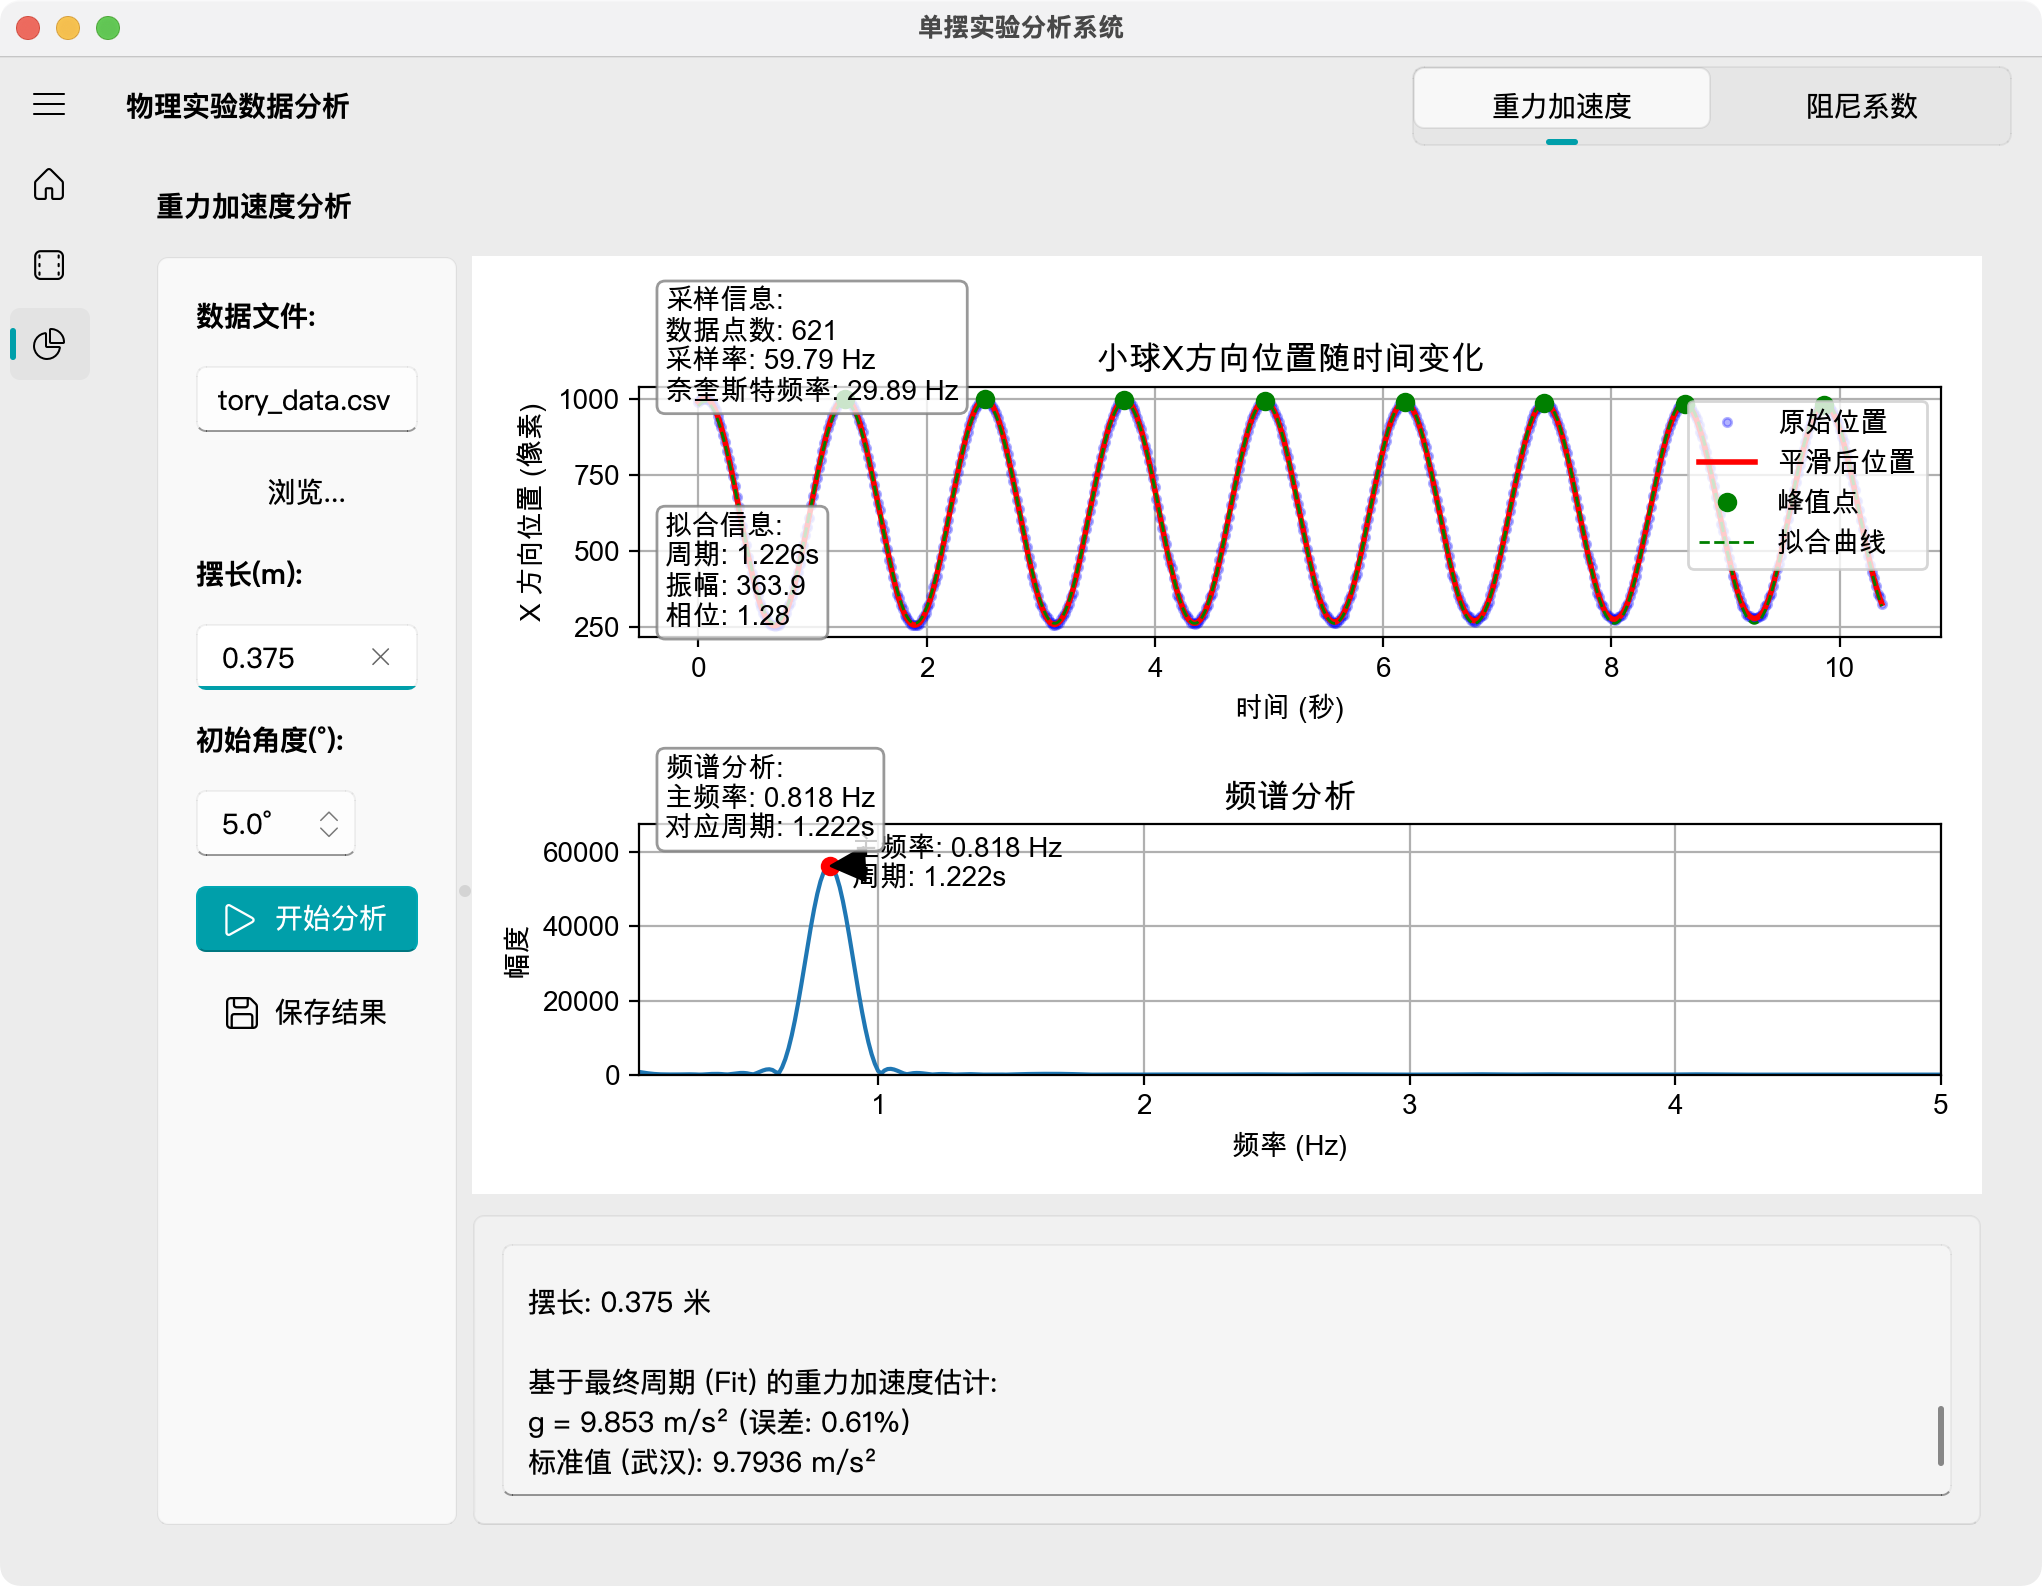
\includegraphics[width=0.5\textwidth]{figures/数据分析界面.png}
    \caption{数据分析界面}
    \label{fig:data_analysis}
\end{figure}

\textbf{gui.py模块},该模块实现了整体用户界面,设计了\textbf{直观的交互流程}和\textbf{数据可视化}功能:

\begin{enumerate}
    \item 界面设计:软件采用流体设计语言(Fluent Design),通过亚克力效果(高斯模糊与透明度混合)创建深度感和层次感,增强用户体验。界面组件如导航栏、卡片和按钮均采用圆角设计,配合动态阴影和悬停效果,提供现代化的视觉体验。      
    \item 数据可视化技术:系统整合matplotlib绘图库,设计了多种可视化图表:
    \begin{enumerate}[label=\alph*.]
        \item 轨迹图:展示小球在二维平面内的运动轨迹,直观反映运动范围和路径;
        \item 位置-时间图:展示位置随时间变化的曲线,并叠加拟合曲线,便于观察振动特性;
        \item 频谱分析图:展示信号频谱,标记主频点,帮助理解振动的频率组成;
        \item 对数衰减图:展示振幅对数值随时间的变化,用于直观观察阻尼特性。
    \end{enumerate}
    
    \item 模块集成机制:系统通过Qt的信号槽机制实现模块间松耦合集成。视频处理完成后自动触发分析模块,分析结果实时更新到界面,形成完整的工作流。这种设计使用户能够在同一界面中完成从视频导入到结果查看的全部操作,大幅提升了实验效率。
\end{enumerate}


\begin{figure}[H]
    \centering
    
\includegraphics[width=0.5\textwidth]{figures/软件界面1.png}
    \caption{软件交互界面展示}
    \label{fig:software_interface}
\end{figure}


通过这种模块化设计,软件实现了从物理现象的观察到物理参数计算的完整流程,使用户能够直观地获取实验数据,进行周期和重力加速度的计算,并可视化实验结果,有效地将AI技术与物理实验教学相结合。

\subsection{系统误差分析}

在实验过程中,除了理论模型和算法带来的误差外,系统性误差也可能影响测量的准确性。这些误差来源多样,涵盖了图像采集和处理、数据处理算法、物理系统、环境因素以及基准值误差等方面。下面将详细分析各类误差的来源及其对实验结果的可能影响。

\subsubsection{图像采集和处理误差}  
在图像采集和处理阶段,主要的误差来源包括以下几点:
(1)YOLO目标检测的定位误差:即使在理想条件下,YOLO目标检测算法也存在一定的误差,这可能导致小球位置的测量不够精确;
(2)摄像机的帧率限制:由于摄像机的帧率有限,采样点可能不足以充分捕捉到小球运动的细节,从而影响周期的准确测量;
(3)摄像机的视角误差:如果摄像机未能完全垂直于单摆的运动平面,则会产生投影误差,进而影响位置的测量;
(4)镜头畸变:相机镜头的畸变可能在图像边缘产生系统性偏差,这些畸变可能导致边缘区域的位置测量不准确,进而影响整个实验的结果。

\subsubsection{数据处理算法误差}  
在数据处理过程中,主要的误差来源有以下几点:
(1)平滑处理带来的误差:使用Savitzky-Golay滤波器进行数据平滑时,虽然有效地减少了噪声,但也可能稍微改变信号的相位和幅度,从而影响周期的测量;
(2)FFT分析的频率分辨率问题:FFT分析的频率分辨率限制可能导致无法准确捕捉低频信号;
(3)峰值检测误差:峰值检测法在噪声较大的情况下可能出现误判,导致周期测量误差;
(4)曲线拟合误差:曲线拟合假设简谐运动模型,但实际运动受阻尼等因素影响,模型与实际情况的不完全契合可能导致周期测量误差。

\subsubsection{物理系统误差}  
物理系统中的误差主要来源于以下几个方面:
(1)大摆角误差:本实验的测量原理是基于小摆角近似,但实际实验中如果摆角较大,会导致测量结果存在误差,虽然程序中采用了大摆角修正,但该修正公式依然是近似的;
(2)摆长测量误差:摆长被定义为从支点到摆球质心的距离,但由于摆球并非理想质点,且绳子本身具有一定的弹性,这些因素可能导致摆长测量不准确,进而影响重力加速度的计算;
(3)空气阻力影响:实验模型假设了简谐运动,但实际上空气阻力会导致振幅逐渐减小,从而影响周期的测量,特别是在较长时间的实验中,空气阻力的影响不可忽视。


\subsubsection{环境因素}  
环境因素是另一重要的误差来源,具体包括以下几点:
(1)温度变化对摆长的影响:温度变化可能导致绳子长度的微小变化,进而影响周期的测量精度;
(2)空气密度变化:空气密度的变化会影响空气阻力的大小,进而影响实验结果;
(3)支点摩擦:理想情况下假设支点无摩擦力,但实际上支点摩擦力矩的存在会影响小球的运动,进而影响测量结果;
(4)外部振动:实验环境中的外部震动可能影响测量的精度,尤其在高精度测量中,这一因素的影响需要特别注意。

\subsubsection{基准值误差}  
基准值误差主要体现在重力加速度的基准值选择上。代码中使用的是武汉地区的标准重力加速度(9.7936 m/s²),但实际实验地点的重力加速度可能存在差异。具体来说,实验地点的海拔高度和纬度等因素会影响当地的重力加速度值,这可能导致实验结果的误差。 
\section{数据测量}


本节介绍借助AI技术对单摆运动进行精确测量,获取用于计算重力加速度和阻尼系数的实验数据的实验步骤。

\subsection{实验装置准备}

将单摆装置放置在平稳桌面上,确保支架稳固,摆动时不会晃动;周围环境稳定,没有明显的振动和气流干扰小球的自然摆动。

\subsection{实验视频采集}

\begin{enumerate}[leftmargin=*]
    \item 相机设置与固定:
    \begin{itemize}
        \item 使用智能手机或数码相机,设置分辨率为1080p,帧率为60 FPS;
        \item 使用三脚架固定相机位置,确保镜头与单摆摆动平面严格平行;
        \item 调整相机距离,使单摆装置位于画面中央,且整个摆动过程都在视野范围内;
    \end{itemize}
    
    \item 初始条件设置:
    \begin{itemize}
        \item 使用精密刻度尺测量摆长$l$(从支点到摆球质心的距离),精确到毫米级,记录数值;
        \item 将摆球拉至特定初始角度$\theta_0$;
        \item 使用角度测量工具(如量角器)或底座刻度盘记录精确的初始角度值;
    \end{itemize}
    
    \item 视频拍摄执行:
    \begin{itemize}
        \item 轻柔释放摆球,避免施加额外力量,待摆球稳定摆动后开始拍摄;
        \item 拍摄时长:
        \begin{itemize}
            \item 重力加速度测量:保持拍摄至少5-10个完整周期(约10-20 s),提高统计精度;
            \item 阻尼系数测量:拍摄15-20个完整周期(约20-30 s),以充分捕捉振幅衰减过程;
        \end{itemize}
        \item 整个拍摄过程中保持环境安静,避免外部振动和气流干扰;
    \end{itemize}
    
    \item 多组数据采集:
    \begin{itemize}
        \item 重力加速度测量:重复测量摆长$l$,重复上述过程获取5组独立的实验视频,减小偶然误差;
        \item 阻尼系数测量:将摆长设置为0.8 m,重复上述过程获取5组独立的实验视频。
    \end{itemize}
\end{enumerate}
\begin{figure}[H]
    \centering
    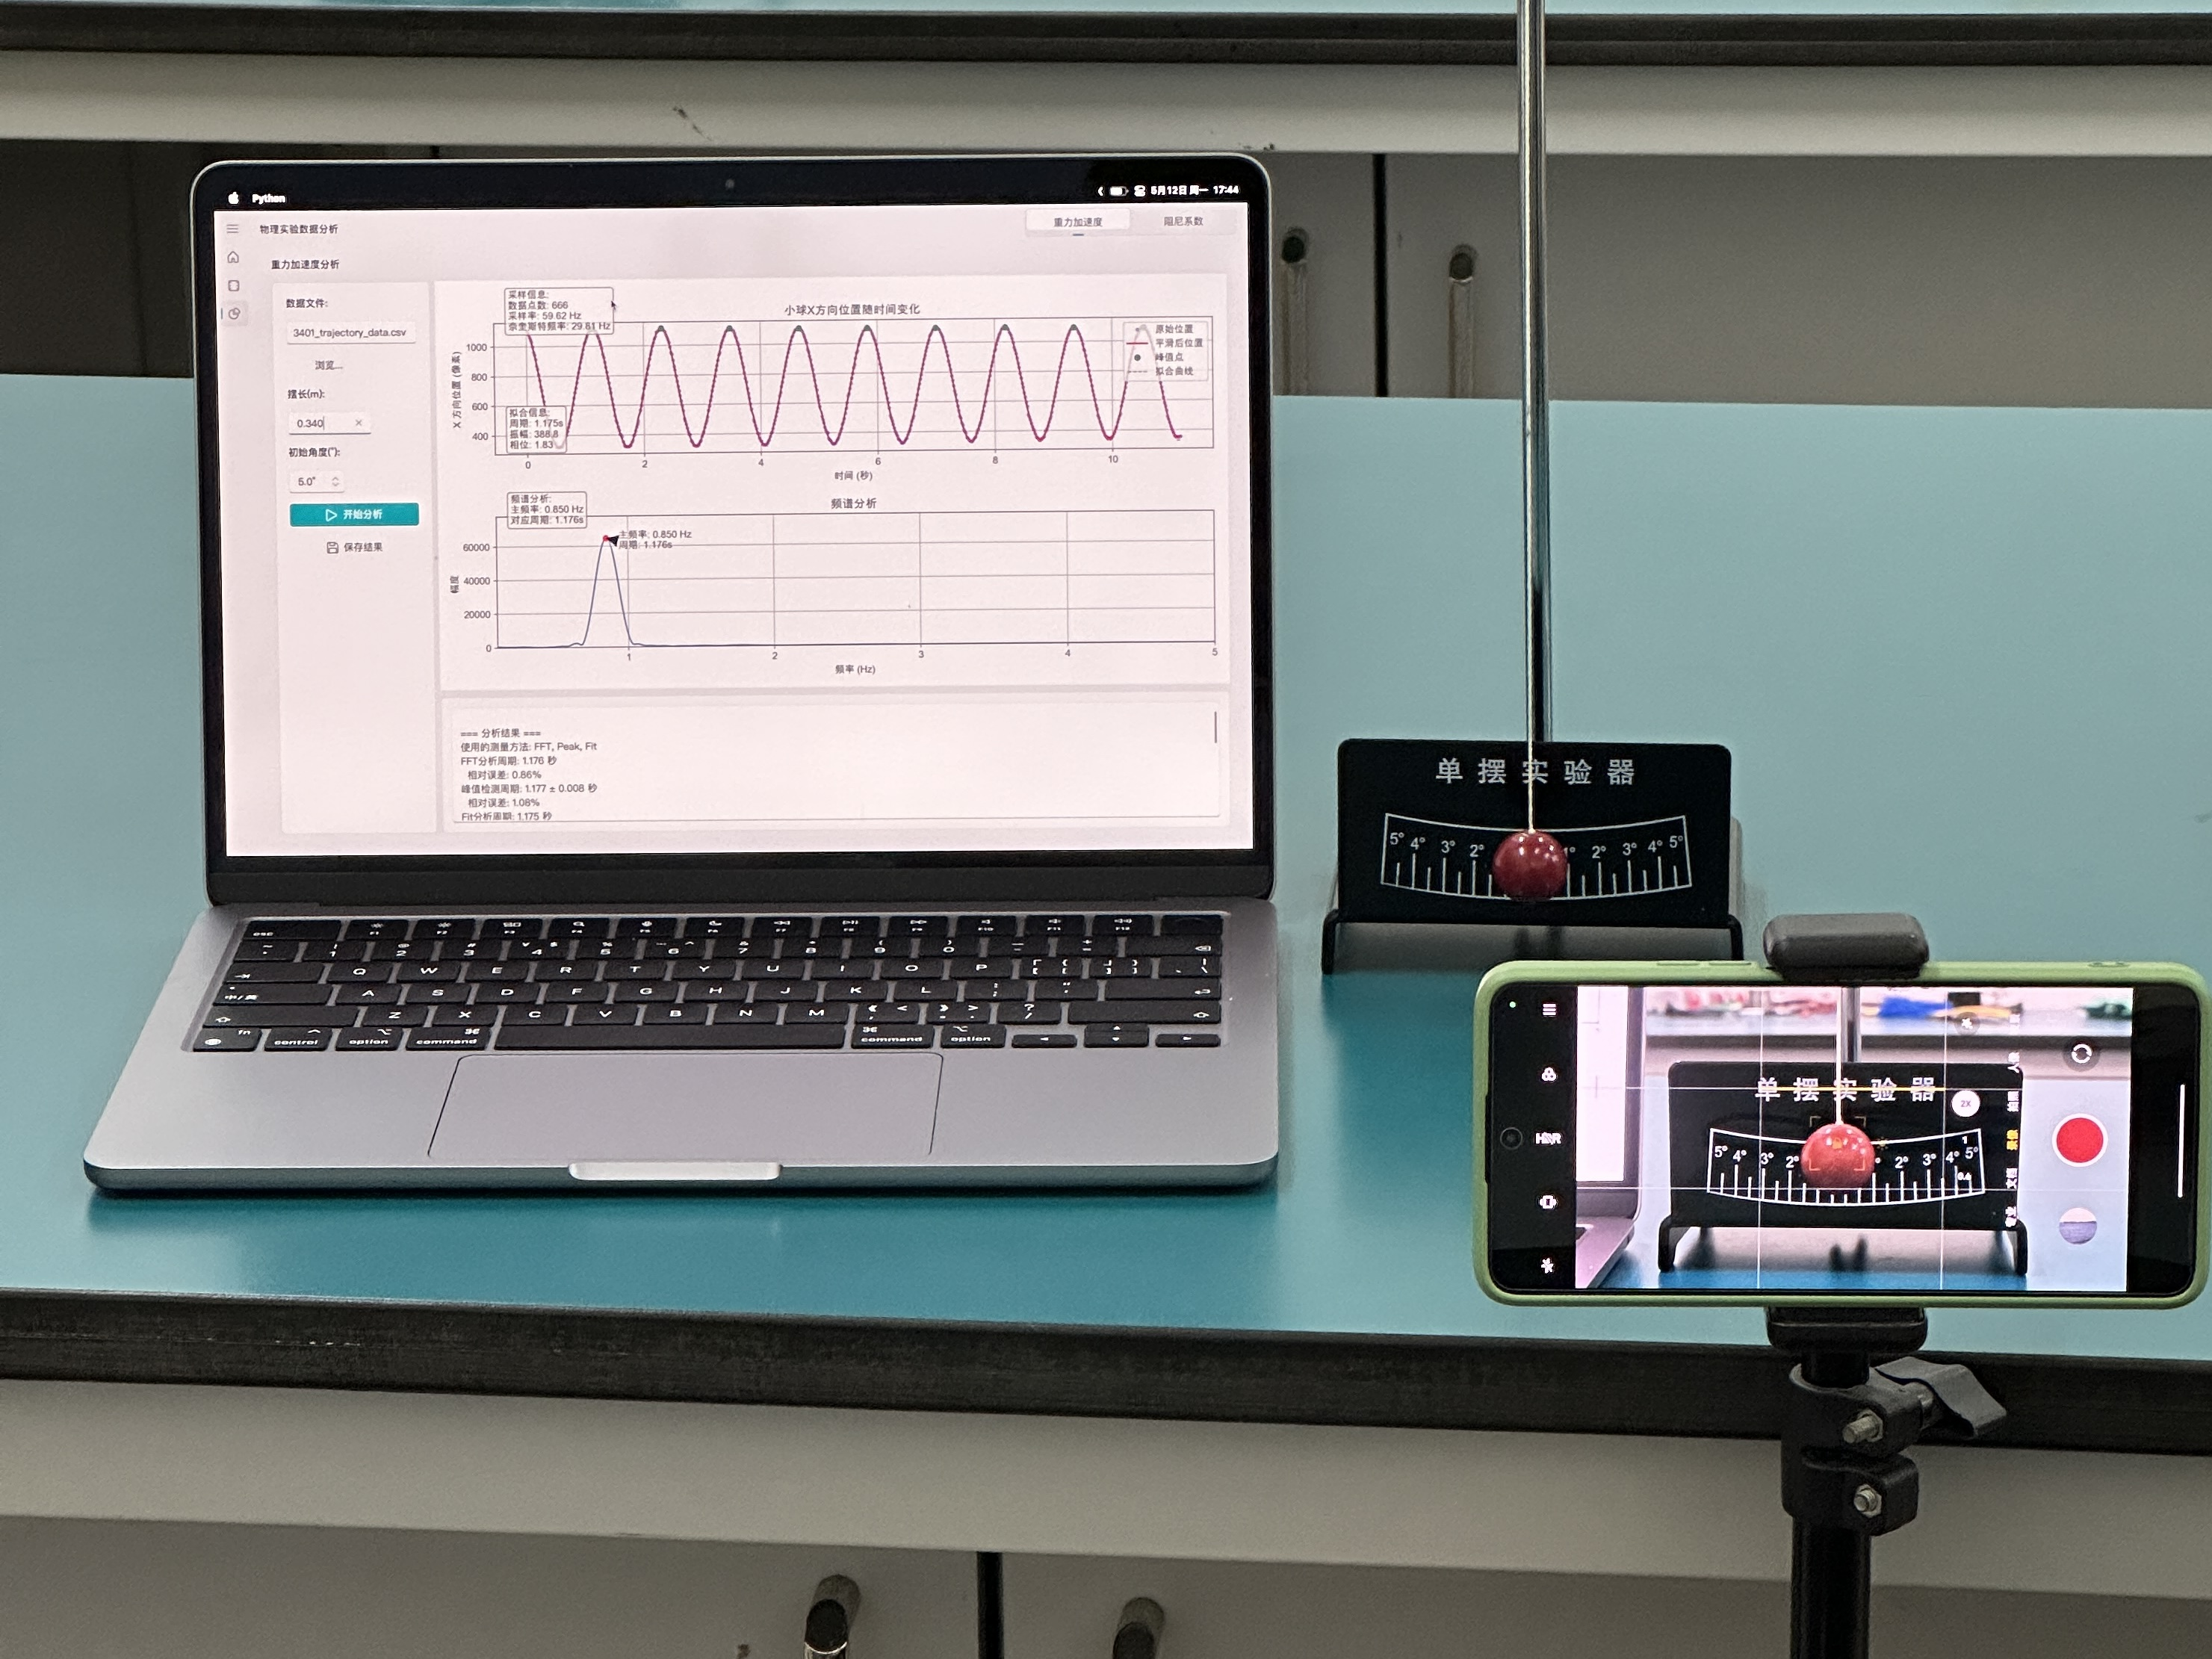
\includegraphics[width=0.6\textwidth]{figures/实验画面.JPG}
    \caption{实验数据采集过程}
    \label{fig:experiment_process}
\end{figure}

\subsection{实验数据处理与记录}

\begin{enumerate}[leftmargin=*]
    \item 软件初始化:启动实验分析软件,进入"视频处理"模块;
    
    \item 参数配置:
    \begin{itemize}
        \item 导入实验视频文件(支持MP4、AVI等主流格式);
        \item 载入训练完成的YOLO模型权重文件(默认为best.pt);
        \item 设置置信度阈值(默认为0.5,若检测效果不佳,可适当调低);
    \end{itemize}
    
    \item 数据提取执行:设置完参数后,点击"开始处理"按钮,启动AI识别模型,
    \begin{itemize}
        \item 观察实时预览窗口中摆球的检测框,确认跟踪稳定;
        \item 系统自动从每一帧提取摆球中心坐标,生成时间-位置原始数据集,保存为CSV格式文件;
        \item 处理完成后,点击结果文件夹按钮,可查看结果视频、轨迹图、位置-时间数据集;
    \end{itemize}

    \item 数据记录:
    \begin{itemize}
        \item 得到摆球位置-时间数据集文件后,进入"数据分析"模块;
        \item 选择分析模式:
        \begin{itemize}
            \item 重力加速度测量:选择"重力加速度测量"模式,输入摆长$l$与初始角度$\theta_0$,系统自动计算周期$T$与重力加速度$g$;
            \item 阻尼系数测量:选择"阻尼振动分析"模式,系统自动拟合振幅衰减曲线,计算阻尼系数$\beta$;
        \end{itemize}
        \item 将相关数据记录于实验记录表中。
    \end{itemize}   
\end{enumerate} 

\begin{figure}[H]
    \centering
    \subfigure[重力加速度测量结果]{
        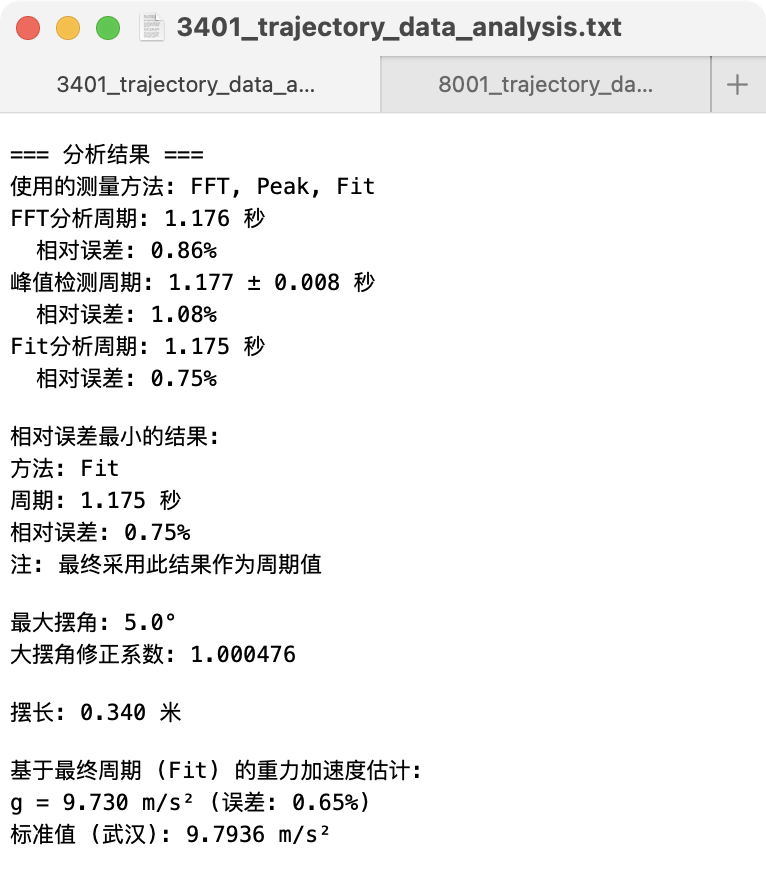
\includegraphics[width=0.4\textwidth]{figures/测量结果1.png}
        \label{fig:measurement_result1}
    }
    \subfigure[阻尼系数测量结果]{
        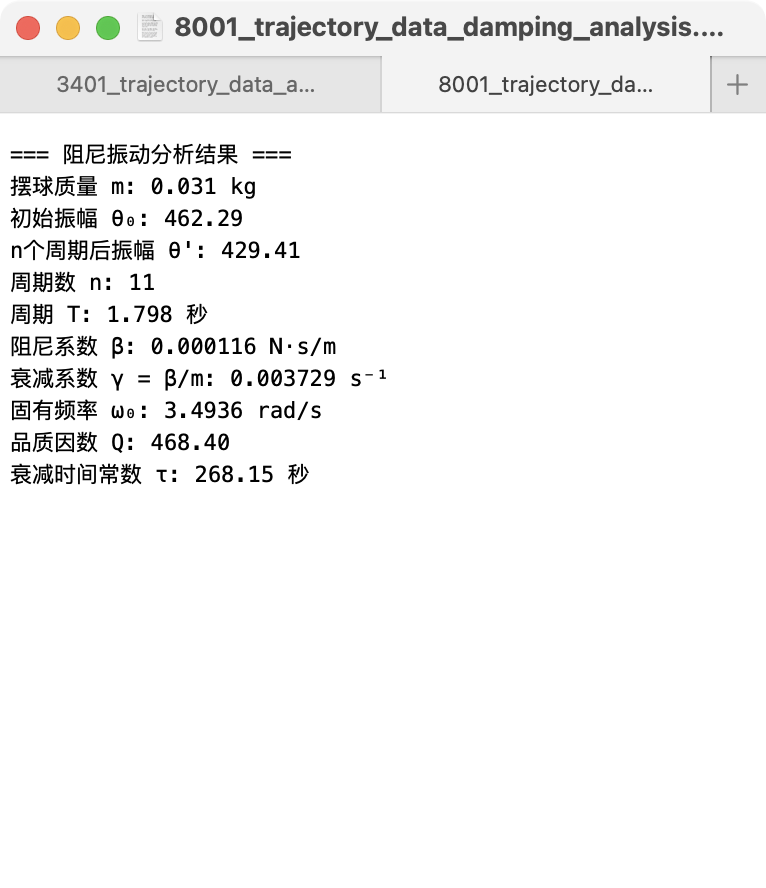
\includegraphics[width=0.4\textwidth]{figures/测量结果2.png}
        \label{fig:measurement_result2}
    }
    \caption{实验测量结果示例}
    \label{fig:measurement_results}
\end{figure}


\section{数据分析}

通过该AI辅助系统,本团队获得了大量高精度的实验数据。本节将详细分析这些数据,验证系统的有效性,并展示实验结果,验证相关物理规律。


\subsection{重力加速度测量的数据分析}


\subsubsection{重力加速度测量结果与对比}
本实验通过AI视觉跟踪技术测量单摆运动,实现了高精度重力加速度测定。实验使用摆长约0.35m,初始摆角5°,进行了5组重复测量,测量结果如下:

\begin{table}[H]
\centering
\caption{重力加速度多次测量结果汇总}
\begin{tabular}{@{}c c c c c c@{}}
\toprule
\textbf{实验编号} & \textbf{摆长(m)} & \textbf{测量方法} & \textbf{周期(s)} & \textbf{重力加速度(m/s$^2$)} & \textbf{相对误差(\%)} \\
\midrule
3501 & 0.3505 & FFT & 1.191 & 9.748 & 0.47 \\
3502 & 0.3501 & FFT & 1.189 & 9.781 & 0.12 \\
3503 & 0.3499 & FFT & 1.187 & 9.815 & 0.22 \\
3504 & 0.3495 & Peak & 1.189 & 9.783 & 0.11 \\
3505 & 0.3500 & Fit & 1.188 & 9.796 & 0.02 \\
\bottomrule
\end{tabular}
\label{tab:gravity_results}
\end{table}


根据李本苍等人的研究\textsuperscript{\cite{KJSJ201335139}},传统重力加速测量方法的误差如下:

\begin{table}[H]
\centering
\caption{传统重力加速度测量方法对比(重力加速度标准值9.78995 m/s$^2$)}
\begin{tabular*}{0.7\textwidth}{@{\extracolsep{\fill}} c c c @{}}
\toprule
\textbf{实验方法} & \textbf{测量结果 (m/s$^2$)} & \textbf{相对误差 (\%)} \\
\midrule
平衡法        & $g = 9.623$ & 1.71 \\
单摆法        & $g = 9.609$ & 1.85 \\
复摆法        & $g = 9.704$ & 0.87 \\
倾斜气垫导轨法 & $g = 9.712$ & 0.79 \\
\bottomrule
\end{tabular*}
\label{tab:traditional_methods}
\end{table}
其中平衡法又称阿特伍德机法,是英国剑桥大学数学家、物理学家乔治 •阿特伍德(George Atwood,1746 -1807)为了验证牛顿第二定律,在1784年发表了一篇题为《关于物体的直线运动和转动》的学术论文,提出的一种用于测量加速度及验证牛顿力学定律的机械装置\textsuperscript{\cite{JXWL201706004}},该装置对重力加速的测量精度有所提升,但仪器操作步骤复杂,且误差仍然较大。
\begin{figure}[H]
    \centering
    \subfigure[阿特伍德机示意图]{
        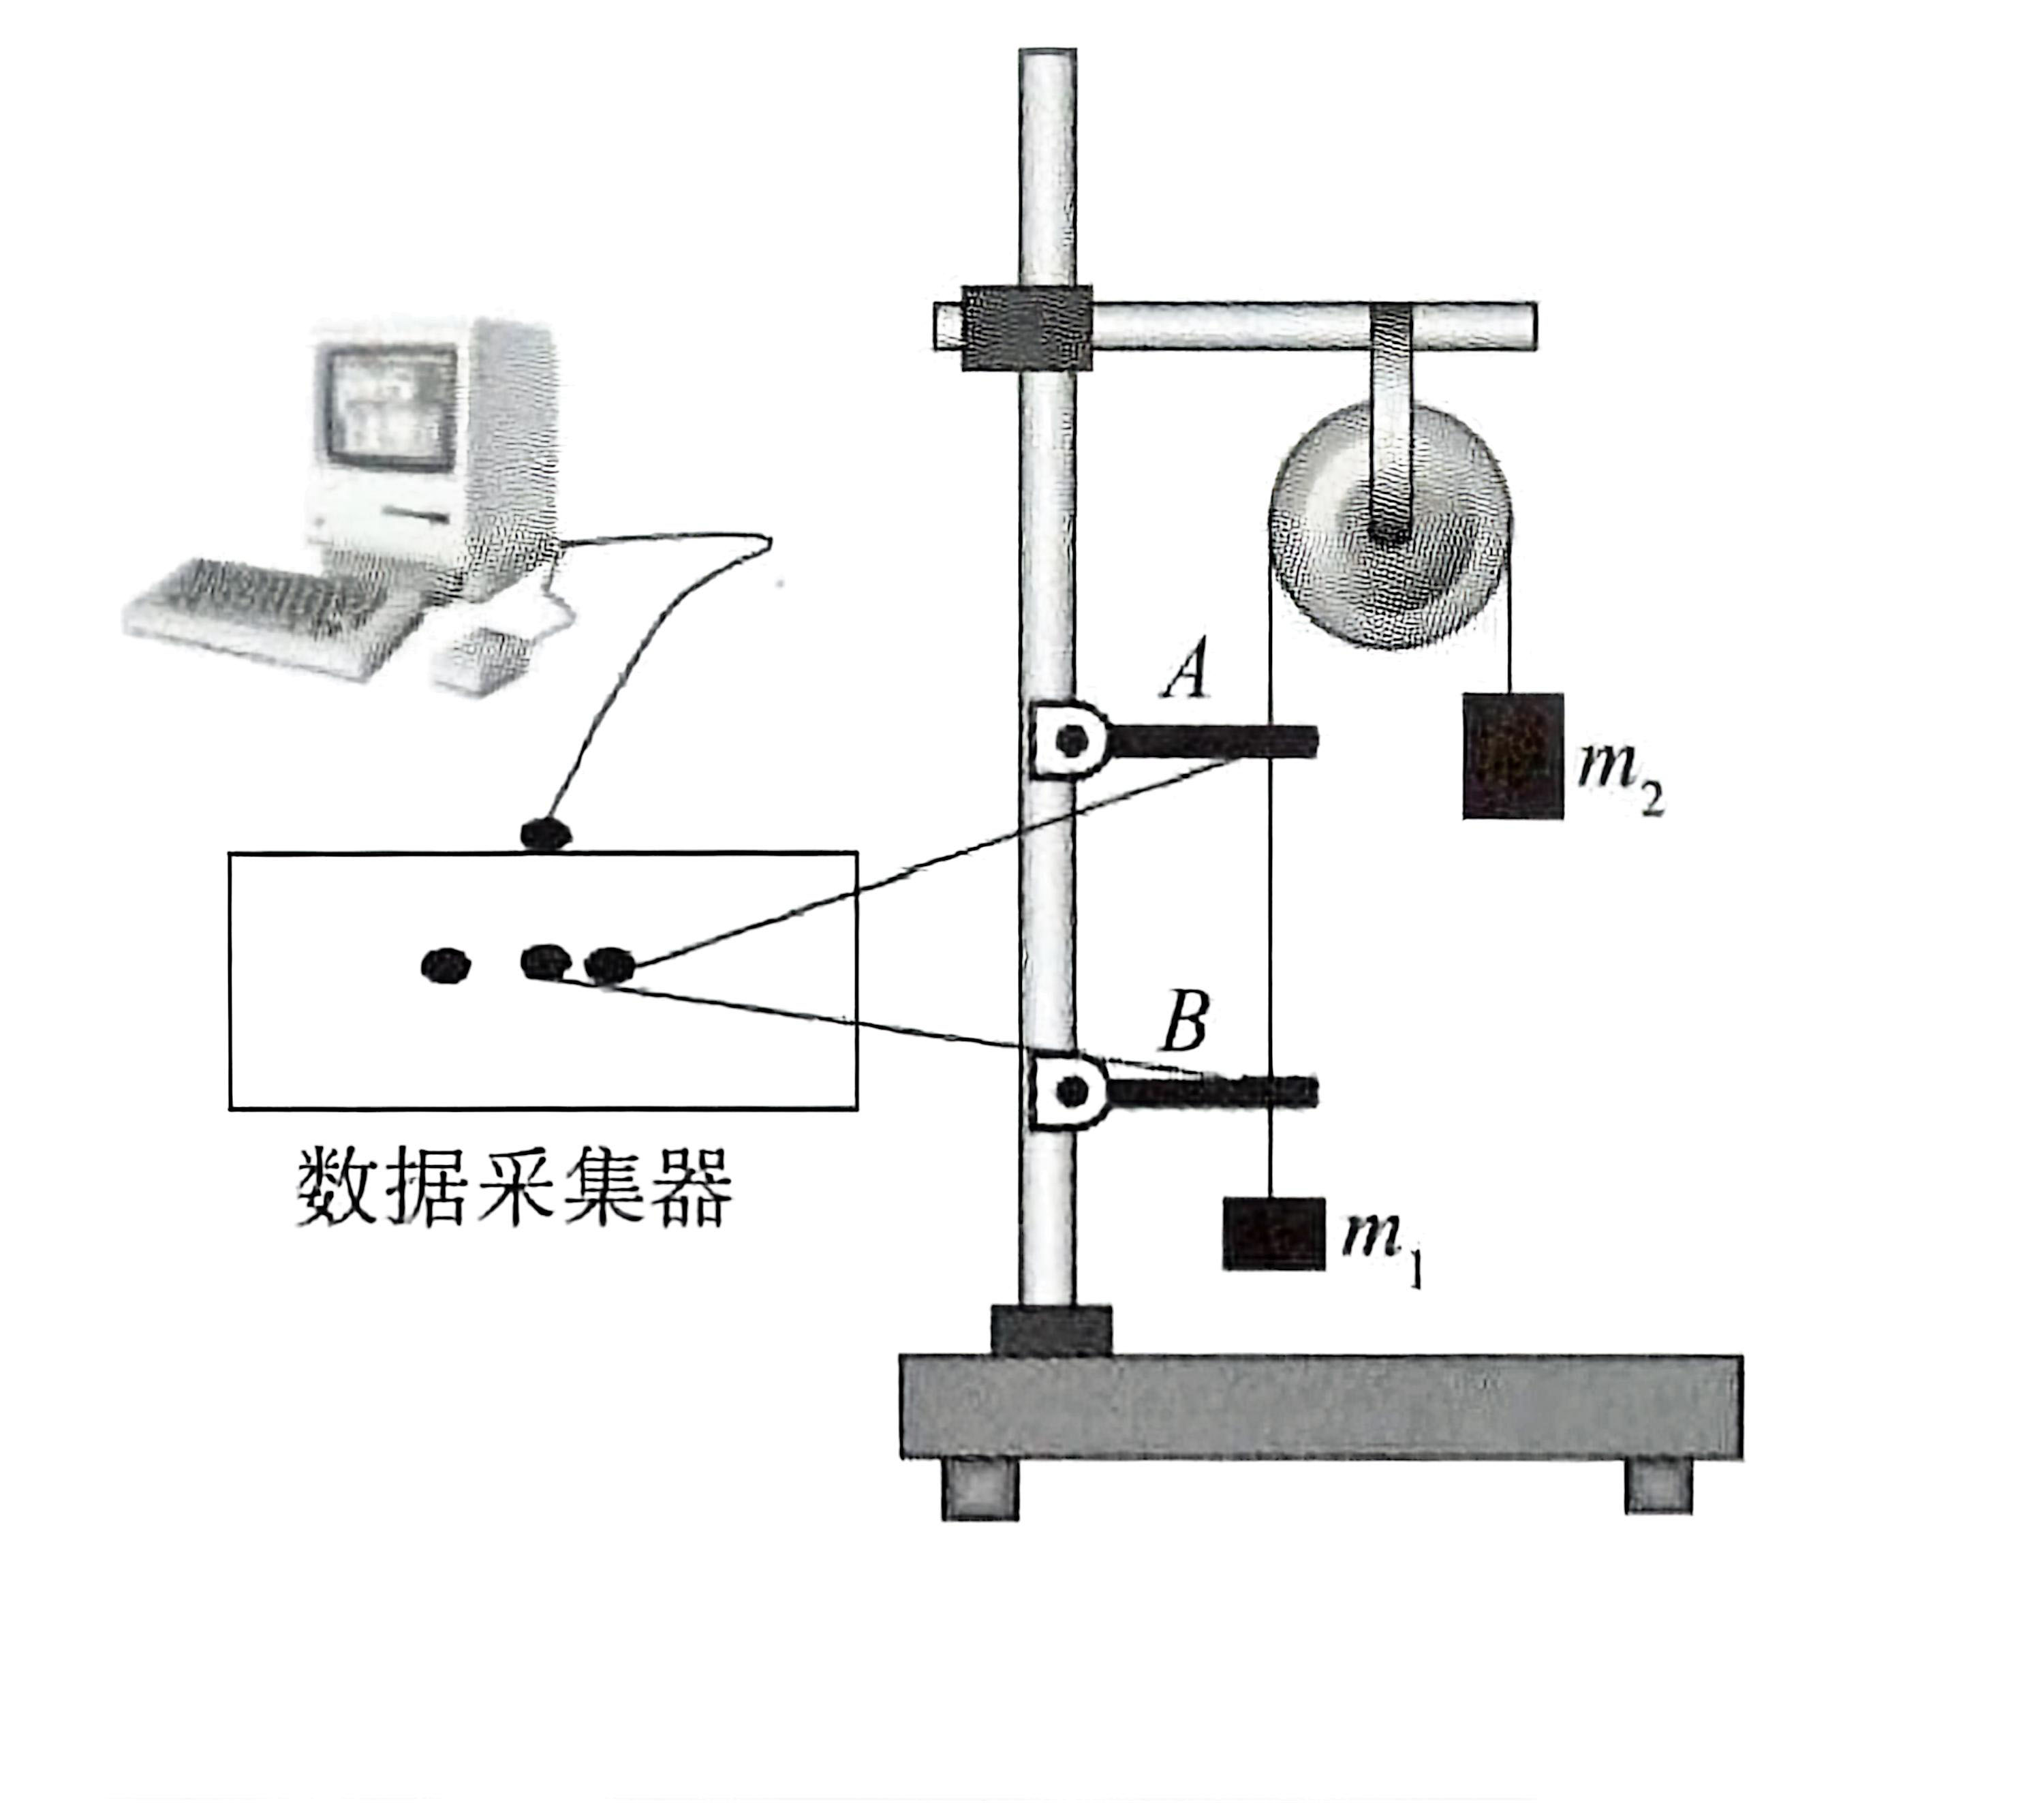
\includegraphics[width=0.4\textwidth]{figures/阿特伍德机示意图.jpg}
        \label{fig:atwood_machine}
    }
    \subfigure[Tracker软件界面]{
        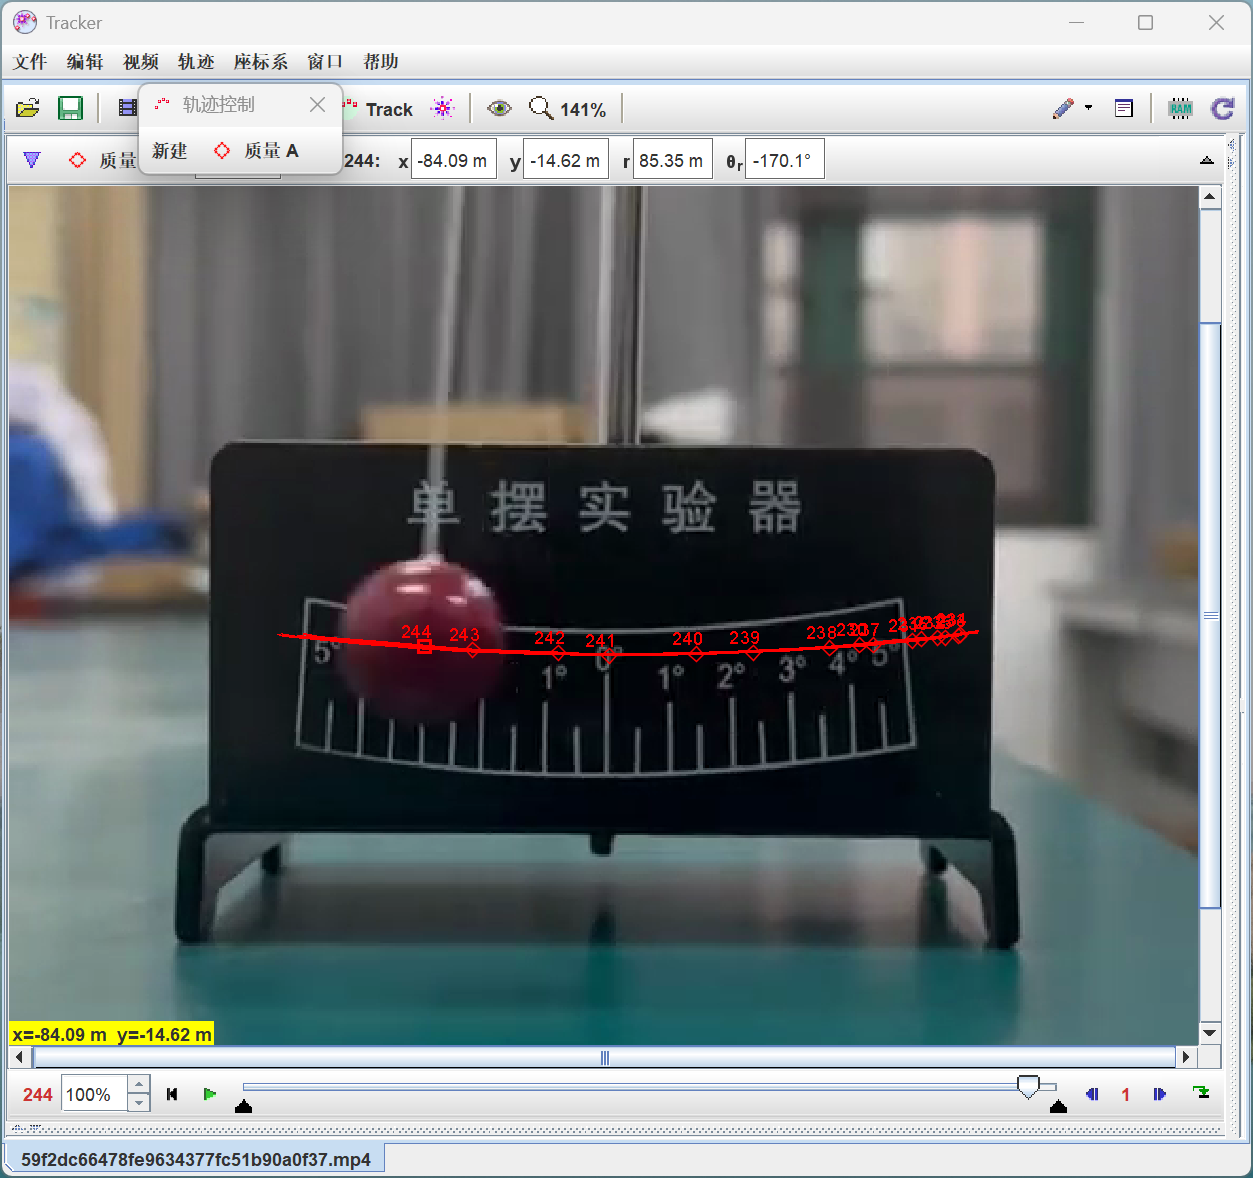
\includegraphics[width=0.4\textwidth]{figures/tracker软件界面.jpg}
        \label{fig:tracker_interface}
    }
    \caption{传统重力加速度测量与分析工具}
    \label{fig:traditional_tools}
\end{figure}


洪炎红等人的研究\textsuperscript{\cite{WLTB201706010}}采用Tracker软件进行重力加速度测量,是一种利用传统计算机视觉技术测量重力加速度的新方法。Tracker是一个基于开源物理(OSP)Java框架的免费视频分析和建模工具\textsuperscript{\cite{brown2009innovative}}。
与Tracker相比,本实验采用的AI辅助系统具有显著优势。本项目采用3502号实验视频,使用本AI辅助系统与Tracker软件分别进行轨迹追踪,将得到的数据文件进行相同的数据处理,对比数据如下:

\begin{table}[H]
\centering
\caption{本系统与Tracker软件对比}
\begin{tabular*}{0.75\textwidth}{@{\extracolsep{\fill}} c c c @{}}
\toprule
\textbf{性能指标} & \textbf{AI辅助系统} & \textbf{Tracker软件} \\
\midrule
识别数据点数 & 631 & 255 \\
测得周期 & 1.189 s & 1.193 s \\
测量精度 & 相对误差为0.12\% & 相对误差为0.85\% \\
背景要求 & 无特殊要求,适应复杂背景 & 需要高对比度,避免杂乱背景 \\
标记要求 & 无需特殊标记物 & 通常需要高对比度标记点 \\
自动化程度 & 全自动跟踪与分析 & 需要手动辅助标记与跟踪 \\
\bottomrule
\end{tabular*}
\label{tab:tracker_comparison}
\end{table}

可见,本系统基于深度学习目标检测算法,能够在无需特殊背景和标记物的情况下精确跟踪运动物体,而Tracker软件通常需要人工设置跟踪点且对背景环境有较高要求。本系统识别目标更加准确,获得了更多的数据点,这为获取高精度实验数据提供了坚实基础,最终的相对误差也显著降低。

\begin{SecondaryBox}[重力加速度测量结果 ]
通过5组数据的综合分析,最终测得的重力加速度平均值为$g = 9.785$ m/s$^2$,与武汉地区标准值$9.7936$ m/s$^2$相比,最佳测量结果的相对误差仅为0.02\%,平均相对误差为0.19\%。测量精度显著优于传统的测量方法,充分证明了AI辅助测量系统的高精度性能。
\end{SecondaryBox}

\subsubsection{周期计算方法对比}

本系统创新性地应用三种互补的周期计算方法,充分利用\textbf{AI赋能的数据收集优势},大幅提高测量精度。以下为摆长0.3501 m、5°初始角度条件下的对比数据:

\begin{table}[H]
\centering
\caption{不同周期计算方法的结果对比(来自3502\_trajectory\_data\_analysis.txt数据)}
\begin{tabular*}{0.9\textwidth}{@{\extracolsep{\fill}} c c c c c@{}}
\toprule
\textbf{计算方法} & \textbf{测量周期(s)} & \textbf{标准差} & \textbf{重力加速度(m/s$^2$)} & \textbf{相对误差(\%)} \\
\midrule
FFT频谱分析法 & 1.189 & - & 9.781 & 0.12 \\
峰值检测法 & 1.192 & 0.007 & 9.740 & 0.55 \\
曲线拟合法 & 1.193 & - & 9.719 & 0.77 \\
最优结果(FFT) & 1.189 & - & 9.781 & 0.12 \\
\bottomrule
\end{tabular*}
\label{tab:period_methods}
\end{table}

如表\ref{tab:period_methods}所示,各种方法测量结果较为接近,但FFT频谱分析法在本例中精度最高。系统默认采用相对误差最小的结果作为最终值。三种方法的特点比较:

\begin{enumerate}[leftmargin=*]
    \item 快速傅里叶变换法:将时域信号转换至频域,通过能量分布识别主频率。本系统采用Hanning窗函数预处理与零填充技术增强频率分辨率,优势是噪声抑制能力强,在5个测量数据中有3次被选为最优方法。在数据3502中表现最佳,相对误差仅为0.12\%;
    
    \item 峰值检测法:直接在时域识别相邻波峰之间的时间差,计算最直观且高效,对于信噪比较高的场景表现良好,但对噪声较敏感。在5个测量数据中有1次被选为最优方法,在数据3504中表现最佳,相对误差为0.11\%;
    
    \item 曲线拟合法:基于物理模型$x(t) = A\sin(\omega t + \phi) + C$,通过非线性最小二乘法拟合,利用全部数据点信息,抗噪性能良好,但拟合结果对初始值敏感,可能存在拟合失败的情况。
\end{enumerate}

\begin{figure}[ht]
    \centering
    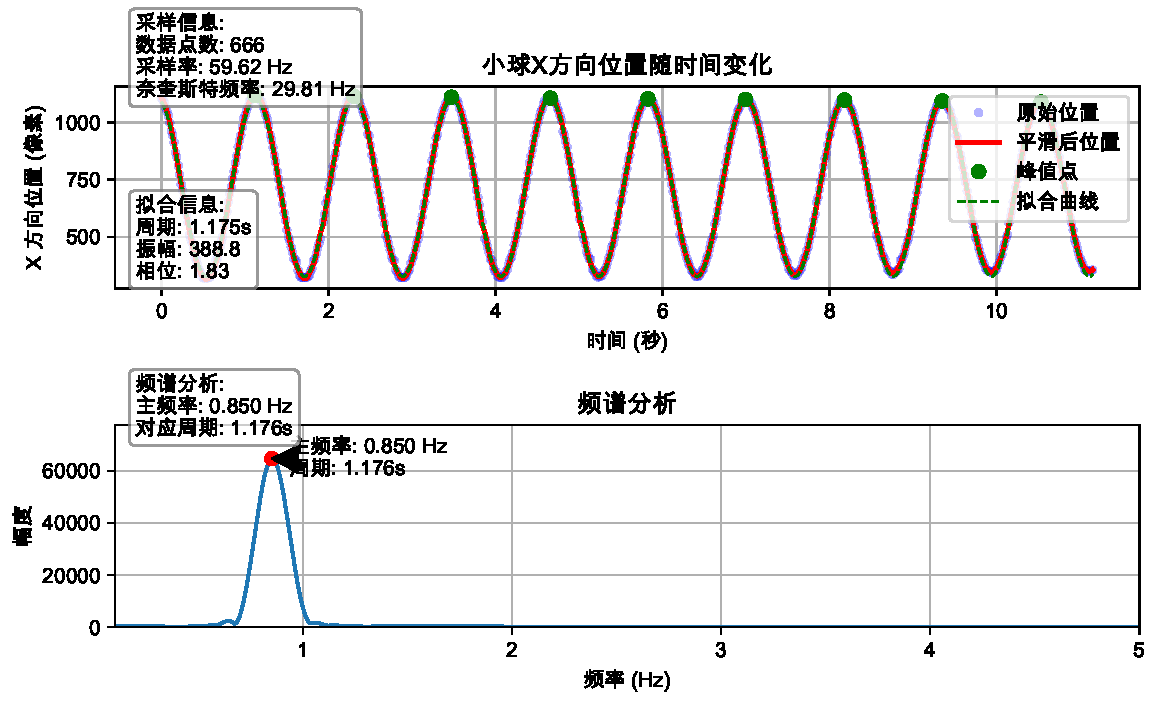
\includegraphics[width=0.7\textwidth]{figures/重力加速度分析结果可视化.pdf}
    \caption{重力加速度测量的波形分析与频谱分析图}
    \label{fig:gravity_analysis}
\end{figure}

如图\ref{fig:gravity_analysis}所示,系统生成的分析图直观显示了平滑后的位置-时间曲线与拟合结果,同时提供频谱分析结果用于验证。观察图中上部可见系统还标记了峰值点位置,用于峰值检测法计算,下部的频谱分析清晰标示出主频率位置。

\subsubsection{摆长与周期的关系分析}

为验证单摆周期公式$T = 2\pi\sqrt{l/g}$,实验采用五组不同摆长(0.33 m-0.37 m)进行测量,通过\textbf{AI视觉跟踪系统获取高精度位置数据},使用多种方法分析周期。实验结果如下:

\begin{table}[H]
\centering
\caption{不同摆长的周期与重力加速度测量结果}
\begin{tabular}{@{}c c c c c@{}}
\toprule
\textbf{摆长(m)} & \textbf{最终周期(s)} & \textbf{采用方法} & \textbf{重力加速度(m/s$^2$)} & \textbf{误差(\%)} \\
\midrule
0.33 & 1.155 & Peak & 9.774 & 0.2 \\
0.34 & 1.174 & FFT & 9.747 & 0.47 \\
0.35 & 1.193 & Fit & 9.725 & 0.7 \\
0.36 & 1.210 & Peak & 9.725 & 0.7 \\
0.37 & 1.225 & FFT & 9.765 & 0.29 \\
\bottomrule
\end{tabular}
\label{tab:lengths_periods}
\end{table}

如表\ref{tab:lengths_periods}所示,对于每个摆长,系统分别使用傅里叶变换法(FFT)、峰值检测法(Peak)和曲线拟合法(Fit)三种方法计算周期,并根据相对误差自动选择最优方法作为最终结果。

将周期$T$对摆长平方根$\sqrt{l}$作图,如图\ref{fig:period_length}所示,呈现出良好的线性关系,符合理论预期。
实验数据点与拟合直线高度吻合,得到拟合方程$T = 2.0463 \cdot \sqrt{l} - 0.0190$,
决定系数$R^2 = 0.9995$,表明线性拟合程度极佳。

\begin{figure}[H]
    \centering
    \begin{tikzpicture}[scale=0.8]
    % 设置坐标系
    \begin{axis}[
        width=0.85\textwidth,
        height=0.6\textwidth,
        xlabel={摆长平方根 $\sqrt{l}$ (m$^{1/2}$)},
        ylabel={周期 $T$ (s)},
        xlabel style={font=\small},
        ylabel style={font=\small},
        xmin=0.565, xmax=0.615,
        ymin=1.14, ymax=1.24,
        tick align=inside,
        xtick={0.57, 0.58, 0.59, 0.60, 0.61},
        ytick={1.15, 1.17, 1.19, 1.21, 1.23},
        ymajorgrids=true,
        xmajorgrids=true,
        grid style={gray!30, solid, line width=0.5pt},
        legend style={at={(0.05,0.95)}, anchor=north west, font=\small, draw},
        tick label style={font=\small},
        title style={font=\bfseries\small}
    ]
    
    % 绘制数据点(带误差棒)
    \addplot[only marks, mark=*, mark size=3pt, mark options={fill=blue}, error bars/.cd, y dir=both, y explicit, 
    error bar style={line width=0.8pt, color=black}, error mark options={line width=0.8pt, mark size=3pt, rotate=90}] 
    coordinates {
        (0.5745, 1.155) +- (0, 0.0012)  % sqrt(0.33)
        (0.5831, 1.174) +- (0, 0.0028)  % sqrt(0.34)
        (0.5916, 1.193) +- (0, 0.0042)  % sqrt(0.35)
        (0.6000, 1.210) +- (0, 0.0042)  % sqrt(0.36)
        (0.6083, 1.225) +- (0, 0.0018)  % sqrt(0.37)
    };
    
    % 绘制拟合线
    \addplot[orange, dashed, line width=1.5pt, domain=0.565:0.615] {2.0463*x - 0.0190};
    
    % 添加图例
    \legend{实验数据, {理论拟合: $T = 2.0463 \cdot \sqrt{l} - 0.0190$,$R^2 = 0.9995$}};
    
    \end{axis}
\end{tikzpicture}
    \caption{周期与摆长平方根的线性关系图}
    \label{fig:period_length}
\end{figure}

\begin{SecondaryBox}[周期与摆长平方根的线性关系]
\quad \quad 从拟合结果可知,斜率$k = 2.0463$,代入$k = 2\pi/\sqrt{g}$,可以反算得到$g = 4\pi^2/k^2 = 9.779$ m/s$^2$。
这一结果与武汉地区标准重力加速度值$9.7936$ m/s$^2$非常接近,相对误差仅为0.15\%。
拟合直线的截距为$-0.0190$,理论上应为零,这一微小偏差可能来源于测量系统的系统误差或摆长测量的零点误差。
\end{SecondaryBox}





\subsubsection{大摆角下非线性修正效果}

大摆角条件下,单摆运动不再满足小角度近似,周期会随振幅增大而增加。系统通过非线性周期修正处理该问题:

\begin{equation}
T = T_0 \cdot (1 + \frac{1}{16}\theta^2 + \frac{11}{3072}\theta^4 + ...)
\end{equation}

其中$T_0$为小摆角条件下的理论周期,$\theta$为弧度制的初始摆角。实验通过一系列不同摆角验证该修正有效性:

\begin{table}[H]
\centering
\caption{不同初始摆角的周期与重力加速度测量结果(摆长0.35 m)}
\begin{tabular}{@{}cccccc@{}}
\toprule
\textbf{初始摆角(°)} & \textbf{未修正g值(m/s$^2$)} & \textbf{未修正误差(\%)} & \textbf{修正系数} & \textbf{修正后g值(m/s$^2$)} & \textbf{修正后误差(\%)} \\
\midrule
5 & 9.716 & 0.79 & 1.000476 & 9.725 & 0.70 \\
10 & 9.758 & 0.36 & 1.001907 & 9.795 & 0.02 \\
15 & 9.751 & 0.43 & 1.004301 & 9.835 & 0.43 \\
20 & 9.679 & 1.17 & 1.007669 & 9.828 & 0.35 \\
25 & 9.604 & 1.93 & 1.012029 & 9.837 & 0.44 \\
\bottomrule
\end{tabular}
\label{tab:angle_periods}
\end{table}

数据表明,\textbf{随着摆角增大,非线性效应逐渐显著}。

\begin{SecondaryBox}[大摆角修正效果分析]
分析表\ref{tab:angle_periods}数据可以发现:

1. 修正系数随摆角增大而增加,从5°时的1.000476增至25°时的1.012029,表明大摆角下非线性效应显著增强。

2. 摆角为5°时,未修正重力加速度值为9.716 m/s²,相对误差为0.79\%;当摆角增至25°时,未修正值下降至9.604 m/s²,相对误差增至1.93\%,可见摆角对测量结果的显著影响。

3. 应用非线性修正后,即使在25°的大摆角下,相对误差也能控制在0.44\%以内,而10°条件下的修正效果最佳,相对误差仅为0.02\%,这表明非线性修正显著提高了大摆角条件下的测量精度。

4. 通过对比三种测量方法(FFT、Peak和Fit),系统能够根据不同摆角条件自动选择最优测量方法,5°和25°时选择Fit方法,10°时选择FFT方法,15°和20°时选择Peak方法,这种智能选择进一步优化了测量结果。
\end{SecondaryBox}

\subsection{阻尼系数测量的数据分析}


\subsubsection{阻尼系数测量的测量结果}
本实验利用AI视觉追踪系统,对摆长为0.8 m、摆球质量为0.004 kg的单摆进行了5次重复阻尼特性测量,获得了高精度的阻尼参数数据。测量结果汇总如下表所示:

\begin{table}[H]
\centering
\caption{摆长为0.8 m的单摆阻尼测量结果}
\begin{tabular}{@{}c c c c c c c@{}}
\toprule
\textbf{编号} & \textbf{初始振幅} & \textbf{$n$周期后振幅} & \textbf{周期数$n$} & \textbf{周期$T$(s)} & \textbf{阻尼系数$\beta$(N·s/m)} & \textbf{时间常数$\tau$(s)} \\
\midrule
1 & 349.46 & 115.53 & 33 & 1.788 & 0.000075 & 53.30 \\
2 & 344.50 & 114.35 & 33 & 1.788 & 0.000075 & 53.49 \\
3 & 347.64 & 115.01 & 33 & 1.789 & 0.000075 & 53.37 \\
4 & 345.50 & 113.87 & 33 & 1.787 & 0.000075 & 53.13 \\
5 & 349.34 & 112.48 & 33 & 1.788 & 0.000077 & 52.06 \\
\textbf{平均值} & 347.29 & 114.25 & - & 1.788 & 0.000075 & 53.07 \\
\textbf{标准差} & 2.22 & 1.16 & - & 0.001 & 0.000001 & 0.57 \\
\bottomrule
\end{tabular}
\label{tab:damping_results}
\end{table}

\begin{SecondaryBox}[阻尼系数测量结果]
从表\ref{tab:damping_results}中可以看出,5次测量结果具有良好的一致性,阻尼系数$\beta$的平均值为0.000075 N·s/m,与同类实验结果相接近。
衰减时间常数$\tau$平均为53.07 s,意味着振幅需要约0.88 min才能衰减至初始值的36.8\%(即$1/e$倍),表明该单摆系统阻尼较小,属于典型的弱阻尼系统。
数据的标准差较小,证明了实验测量的重复性和可靠性,同时也表明AI视觉跟踪系统能够稳定地测量阻尼振动过程。
\end{SecondaryBox}



\subsubsection{阻尼特性量化与参数分析}

系统通过自动追踪摆球位置,提取振幅随时间变化的完整数据,应用指数衰减模型 $A(t) = A_0e^{-\frac{\beta}{m} t}$精确量化阻尼特性,
与传统人工测量相比,系统测量阻尼特性参数的优势体现在:
\begin{enumerate}[leftmargin=*]
    \item 高密度数据采集:传统方法通常仅测量有限几个振幅值点,而本系统可提取视频中每一帧的位置数据,获得连续的阻尼衰减过程;
    
    \item 自动峰值识别:系统自动识别所有波峰并提取振幅值,消除了人工计时与目测误差;
    
    \item 对数衰减法:系统自动计算振幅的对数值并进行线性拟合,从斜率直接获得阻尼系数与质量比值$\beta/m$的相反数,大幅提高量化精度。
\end{enumerate}

如图\ref{fig:damping_analysis}所示,上图展示小球位置随时间变化的阻尼振动曲线及其拟合曲线,下图为振幅对数值随时间变化的线性关系图。对数图的斜率即为阻尼系数的负值,实现了直观的阻尼效应量化。


\begin{figure}[H]
    \centering
    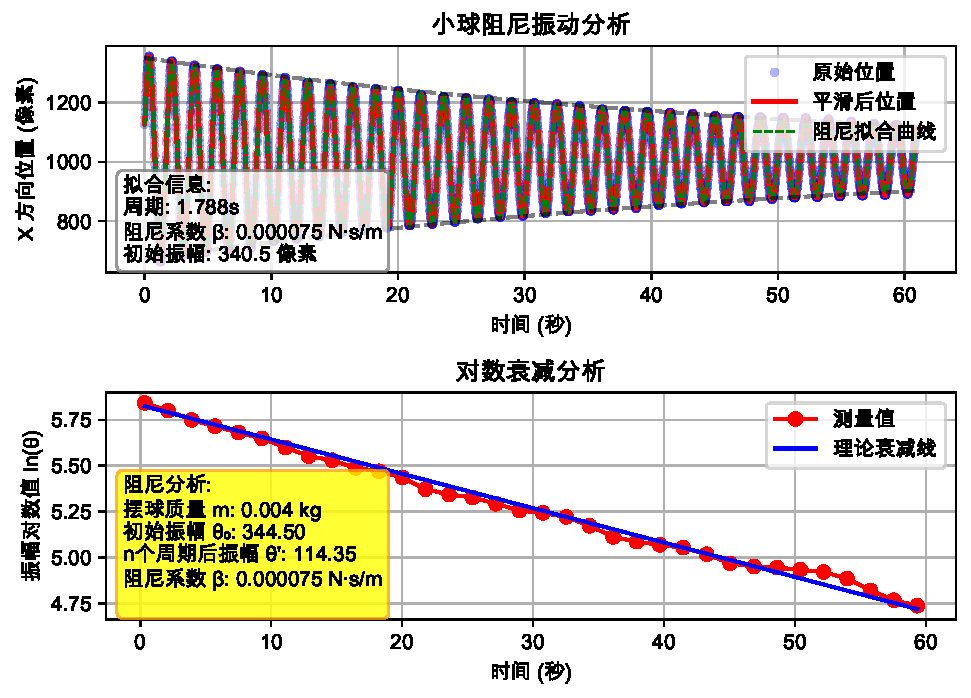
\includegraphics[width=0.65\textwidth]{figures/22_trajectory_data_damping_analysis.pdf}
    \caption{阻尼振动分析与对数衰减图}
    \label{fig:damping_analysis}
\end{figure}



实验在摆长0.8 m条件下进行,获得完整的阻尼参数集,如表\ref{tab:damping_params}所示,

\begin{table}[H]
\centering
\caption{阻尼振动的关键参数测量结果}
\setlength{\tabcolsep}{7mm}
\begin{tabular}[c]{c c c c}
\toprule
{\textbf{参数}} & {\textbf{测量值}} & {\textbf{单位}} \\
\midrule
阻尼系数 $\beta$ & 0.000075 & N$\cdot$s/m \\
固有角频率 $\omega_0$ & 3.5144 & rad/s \\
振动周期 $T$ & 1.788 & s \\
品质因数 $Q$ & 93.26 & 无量纲 \\
衰减时间常数 $\tau$ & 53.07 & s \\
\bottomrule
\end{tabular}
\label{tab:damping_params}
\end{table}

其中品质因数Q\textsuperscript{\cite{DXWL201705004}}:定义为$Q = \frac{m\omega_0}{\beta}$,表征系统振动能量的存储能力,Q值越大表示系统阻尼越小,能量损失率越低。测得Q = 93.26表明该系统属于低阻尼类型;衰减时间常数τ:定义为$\tau = m/\beta$,表示振幅衰减至初始值的1/e所需时间,是量化振动持续时间的重要指标。测得τ = 53.07 s说明该单摆系统能够保持较长时间的振动状态,这两个指标排除出了质量的影响,为探究阻尼特性影响因素提供了参考指标。


\subsubsection{阻尼特性影响因素分析}

为探究影响单摆阻尼特性的主要因素,本团队设计了一系列对比实验,系统分析了摆长、摆球尺寸和摆球质量三个关键因素对阻尼特性的影响。下面将分别详细讨论各因素对阻尼系数($\beta$)、衰减系数($\gamma$)、衰减时间常数($\tau$)、品质因数($Q$)等阻尼特性参数的综合影响。

\textbf{1)摆长对阻尼特性的影响},为探究摆长对阻尼特性的影响,本团队使用固定质量(0.009 kg)的塑料大球,在5°初始摆角条件下,进行了一系列不同摆长(0.4 m至1.0 m)的阻尼特性对比实验。实验结果如表\ref{tab:length_damping}所示。

\begin{table}[H]
\centering
\caption{摆长对阻尼特性的影响}
\begin{tabular}{c c c c c c@{}}
\toprule
\textbf{摆长(m)} & \textbf{周期(s)} & \textbf{阻尼系数$\beta$(N$\cdot$s/m)} & \textbf{衰减系数$\gamma$(s$^{-1}$)} & \textbf{品质因数$Q$} & \textbf{衰减时间常数$\tau$(s)} \\
\midrule
0.40 & 1.278 & 0.000091 & 0.010147 & 484.46 & 98.55 \\
0.55 & 1.496 & 0.000102 & 0.011336 & 370.46 & 88.21 \\
0.70 & 1.683 & 0.000104 & 0.011606 & 321.60 & 86.16 \\
0.85 & 1.855 & 0.000108 & 0.011979 & 282.76 & 83.48 \\
1.00 & 2.004 & 0.000118 & 0.013151 & 238.38 & 76.04 \\
\bottomrule
\end{tabular}
\label{tab:length_damping}
\end{table}

实验数据显示,随着摆长从0.4 m增加到1.0 m:
\begin{itemize}
  \item 振动周期T随摆长增加而显著增加,从1.278 s增至2.004 s,增幅约57\%,符合理论预期$T = 2\pi\sqrt{l/g}$;
  \item 阻尼系数$\beta$随摆长增加而增大约30\%(从0.000091增至0.000118 N·s/m);
  \item 衰减系数$\gamma$(单位质量的阻尼系数)增加约30\%(从0.010147增至0.013151 s$^{-1}$);
  \item 品质因数$Q$显著降低约51\%(从484.46降至238.38);
  \item 衰减时间常数$\tau$降低约23\%(从98.55降至76.04 s);
\end{itemize}

这种变化趋势表明,摆长对单摆系统的阻尼特性有显著影响。摆长增加导致摆球的线速度提高,增加了与空气的相对运动速度,从而增大了空气阻力,表现为阻尼系数的增加。此外,摆长增加改变了整个系统的运动特性,使得能量损耗相对增加,表现为品质因数的降低和衰减时间常数的减小。

\begin{figure}[H]
    \centering
    \subfigure[摆长对阻尼系数的影响]{
        \begin{tikzpicture}[scale=0.5]
    % 设置坐标系
    \begin{axis}[
        width=0.85\textwidth,
        height=0.6\textwidth,
        xlabel={摆长 $l$ (m)},
        ylabel={阻尼系数 $\beta$ (N$\cdot$s/m)},
        xlabel style={font=\small},
        ylabel style={font=\small},
        xmin=0.35, xmax=1.05,
        ymin=0.00008, ymax=0.00012,
        tick align=inside,
        xtick={0.4, 0.55, 0.7, 0.85, 1.0},
        ytick={0.00009, 0.000095, 0.0001, 0.000105, 0.00011, 0.000115, 0.00012},
        yticklabel style={/pgf/number format/fixed, /pgf/number format/precision=6},
        ymajorgrids=true,
        xmajorgrids=true,
        grid style={gray!30, solid, line width=0.5pt},
        legend style={at={(0.05,0.95)}, anchor=north west, font=\small, draw},
        tick label style={font=\small},
        title style={font=\bfseries\small}
    ]
    
    % 绘制数据点
    \addplot[only marks, mark=*, mark size=3pt, mark options={fill=blue}] 
    coordinates {
        (0.40, 0.000091)
        (0.55, 0.000102)
        (0.70, 0.000104)
        (0.85, 0.000108)
        (1.00, 0.000118)
    };
    
    % 绘制拟合线
    \addplot[orange, dashed, line width=1.5pt, domain=0.35:1.05] {0.00004*x + 0.0000766};
    
    % 添加图例
    \legend{实验数据, {线性拟合: $\beta = 4.00 \times 10^{-5} \cdot l + 7.66 \times 10^{-5}$, $R^2 = 0.9395$}};
    
    \end{axis}
\end{tikzpicture}
        \label{fig:length_damping_coef}
    }
    \subfigure[摆长对品质因数的影响]{
        \begin{tikzpicture}[scale=0.5]
    % 设置坐标系
    \begin{axis}[
        width=0.85\textwidth,
        height=0.6\textwidth,
        xlabel={摆长 $l$ (m)},
        ylabel={品质因数 $Q$},
        xlabel style={font=\small},
        ylabel style={font=\small},
        xmin=0.35, xmax=1.05,
        ymin=220, ymax=500,
        tick align=inside,
        xtick={0.4, 0.55, 0.7, 0.85, 1.0},
        ytick={220, 270, 320, 370, 420, 470},
        ymajorgrids=true,
        xmajorgrids=true,
        grid style={gray!30, solid, line width=0.5pt},
        legend style={at={(0.95,0.95)}, anchor=north east, font=\small, draw},
        tick label style={font=\small},
        title style={font=\bfseries\small}
    ]
    
    % 绘制数据点
    \addplot[only marks, mark=*, mark size=3pt, mark options={fill=blue}] 
    coordinates {
        (0.40, 484.46)
        (0.55, 370.46)
        (0.70, 321.60)
        (0.85, 282.76)
        (1.00, 238.38)
    };
    
    % 绘制二次拟合线 (使用MATLAB代码中计算的系数)
    \addplot[orange, dashed, line width=1.5pt, domain=0.35:1.05] {473.84*x^2 - 1049.95*x + 820.99};
    
    % 添加图例
    \legend{实验数据, {二次拟合: $Q = 473.84 l^2 - 1049.95 l + 820.99$, $R^2 = 0.9854$}};
    
    \end{axis}
\end{tikzpicture}
        \label{fig:length_quality_factor}
    }
    \caption{摆长对阻尼系数和品质因数的影响}
    \label{fig:length_damping}
\end{figure}

如图\ref{fig:length_damping}所示,阻尼系数$\beta$与摆长呈增长关系,而品质因数$Q$则随摆长增加而显著下降。

\textbf{2)摆球尺寸对阻尼特性的影响},为探究摆球尺寸对阻尼特性的影响,本团队使用两种不同直径的塑料球进行对比实验,并保持摆长(0.8m)不变,为排除质量的影响,本团队主要分析衰减系数$\gamma$、品质因数$Q$和衰减时间常数$\tau$。实验结果如表\ref{tab:size_damping}所示。

\begin{table}[H]
\centering
\caption{摆球尺寸对阻尼特性的影响}
\begin{tabular}{c c c c c c@{}}
\toprule
\textbf{球类型} & \textbf{质量(kg)} & \textbf{阻尼系数$\beta$(N$\cdot$s/m)} & \textbf{衰减系数$\gamma$(s$^{-1}$)} & \textbf{品质因数$Q$} & \textbf{衰减时间常数$\tau$(s)} \\
\midrule
塑料小球 & 0.004 & 0.000089 & 0.022295 & 157.90 & 44.86 \\
塑料大球 & 0.009 & 0.000104 & 0.011508 & 307.46 & 86.98 \\
\bottomrule
\end{tabular}
\label{tab:size_damping}
\end{table}

实验数据显示,随着球体尺寸增大(质量从0.004 kg增至0.009 kg):
\begin{itemize}
  \item 衰减系数$\gamma$(单位质量的阻尼系数)降低约48\%(从0.022295降至0.011508 s$^{-1}$);
  \item 品质因数$Q$提高约95\%(从157.90增至307.46);
  \item 衰减时间常数$\tau$提高约94\%(从44.86增至86.98 s);
\end{itemize}

\textbf{3)摆球质量对阻尼特性的影响},为研究质量对阻尼特性的影响,本团队比较了两种不同质量的相同尺寸摆球:不锈钢小球(0.031 kg)和塑料小球(0.004 kg),实验过程中保持摆长(0.8 m)和初始角度(5°)不变。实验结果如表\ref{tab:material_damping}所示。

\begin{table}[H]
\centering
\caption{摆球质量对阻尼特性的影响}
\begin{tabular}{@{}c c c c c c@{}}
\toprule
\textbf{摆球类型} & \textbf{质量(kg)} & \textbf{阻尼系数$\beta$(N$\cdot$s/m)} & \textbf{衰减系数$\gamma$(s$^{-1}$)} & \textbf{品质因数$Q$} & \textbf{衰减时间常数$\tau$(s)} \\
\midrule
不锈钢小球 & 0.031 & 0.000115 & 0.0037 & 941.40 & 269.39 \\
塑料小球 & 0.004 & 0.000089 & 0.0223 & 157.90 & 44.86 \\
\bottomrule
\end{tabular}
\label{tab:material_damping}
\end{table}

实验数据表明,在相同摆长和初始角度条件下,两种不同质量的相同尺寸摆球表现出显著不同的阻尼特性:
\begin{itemize}
  \item 阻尼系数$\beta$随质量增大而略微增大(从0.000089增至0.000115 N·s/m),增幅约29\%
  \item 衰减系数$\gamma=\beta/m$随质量增大而显著降低,塑料球(0.0223 s$^{-1}$)约为不锈钢球(0.0037 s$^{-1}$)的6倍
  \item 不锈钢球的品质因数$Q$远高于塑料球,为941.40,是塑料球(157.90)的约6倍
  \item 不锈钢球的衰减时间常数$\tau$显著长于塑料球,达269.39 s,是塑料球(44.86 s)的约6倍
\end{itemize}

通过对摆长、摆球尺寸和摆球质量三个因素的系统研究,得出以下结论:
\begin{SecondaryBox}[阻尼特性影响因素分析]

1. 摆长对阻尼特性的影响:
   实验表明,摆长从0.4 m增加至1.0 m时,阻尼系数$\beta$增大约30\%,品质因数$Q$下降约51\%,衰减时间常数$\tau$减小约23\%。这一现象可归因于摆长增加导致摆球线速度增大,从而增强了与速度相关的空气阻力,加快了系统能量的耗散速率。

2. 摆球尺寸对阻尼特性的影响:
   对于相同材质的摆球,当尺寸增大时,衰减系数$\gamma$降低约48\%,品质因数$Q$和衰减时间常数$\tau$均提高约95\%。这是因为摆球质量(与半径的三次方成正比,$\propto r^3$)增长速率快于其横截面积(与半径的平方成正比,$\propto r^2$),导致单位质量所受阻尼减小,系统惯性增强。

3. 摆球质量对阻尼特性的影响:
   实验数据显示,相同尺寸条件下,不锈钢球的衰减系数$\gamma$仅为塑料球的约1/6,品质因数$Q$和衰减时间常数$\tau$约为塑料球的6倍。这主要是因为在相似的空气阻力作用下,不锈钢球质量(0.031 kg)显著大于塑料球(0.004 kg),使得单位质量的能量损耗率大幅降低。

\quad\quad 综上所述,摆长主要通过改变摆球运动速度影响系统的绝对阻尼大小,而摆球的尺寸和材质则通过改变质量与截面积的比值影响单位质量的阻尼效应。实验结果表明,密度越高、尺寸越大的摆球,其维持振动的能力越强,表现为更高的品质因数和更长的衰减时间常数。
\end{SecondaryBox}
\section{性能指标}
\subsection{测量范围}
本系统能够测量的物理量及其范围如下:

\begin{table}[ht]
\centering
\caption{系统测量参数范围与精度}
\begin{tabular}{@{}c c c c@{}}
\toprule
\textbf{测量参数} & \textbf{测量范围} & \textbf{分辨率} & \textbf{限制因素} \\
\midrule
单摆周期 $T$ & 0.5 s - 10 s & 16.7 ms & 摄像机帧率 \\
单摆摆长 $l$ & 0.3 m - 1.2 m & 0.001 m & 视觉识别精度 \\
振幅角度 $\theta$ & $0.1^{\circ}$ - $45^{\circ}$ & $0.1^{\circ}$ & 视觉识别精度 \\
阻尼系数 $\beta$ & 0.00001 - 1.0 N$\cdot$s/m & 0.00001 N$\cdot$s/m & 多周期振幅衰减测量精度 \\
\bottomrule
\end{tabular}
\label{tab:measurement_range}
\end{table}

系统测量范围的主要特性与限制:

\begin{enumerate}[leftmargin=*]
    \item 周期测量范围:系统可测量0.5 s至10 s的单摆周期,覆盖了教学实验中常见的摆长范围(0.1 m至2.5 m)。系统最小分辨率受限于摄像机帧率(60 FPS下为16.7 ms)。
    
    \item 摆长测量范围:系统支持0.3 m至1.2 m的摆长测量,摆长过短时,周期较小,受限于摄像机帧率;摆长过长时,摆球运动过快,并且圆锥摆效应显著,影响测量精度。
    
    \item 振幅测量范围:系统支持$0.1^{\circ}$至$45^{\circ}$的振幅角测量。较大振幅($>45^{\circ}$)下会产生明显非线性效应,超出小角度近似适用范围;极小振幅($<0.1^{\circ}$)下像素分辨率成为限制因素。
        
    \item 阻尼特性测量:系统可精确捕捉0.00001至1.0 N$\cdot$s/m范围内的阻尼系数变化,适用于空气阻尼和额外阻尼装置的测量。高阻尼环境(如液体中)需使用专用摄像设备。
\end{enumerate}


\subsection{不确定度}
本项目中涉及到两类不确定度计算:A类不确定度(统计分析法)和B类不确定度(非统计分析法)。

\subsubsection{不确定度基本原理与公式}

\paragraph{A类不确定度}
A类不确定度是通过统计分析一组重复测量数据得到的标准不确定度,其计算公式为:

\begin{equation}
u_A(x) = \sqrt{\frac{\sum_{i=1}^{n}(x_i-\bar{x})^2}{n(n-1)}}
\end{equation}

其中:$x_i$ 为第i次测量结果,$\bar{x}$ 为n次测量的算术平均值,$n$ 为测量次数。

\paragraph{B类不确定度}
B类不确定度是根据仪器精度、系统误差等非统计方法评估的不确定度,计算公式为:

\begin{equation}
u_B(x) = \frac{\Delta x}{\sqrt{3}}
\end{equation}

其中$\Delta x$为测量仪器的分辨力或最大允差。

\paragraph{合成不确定度}
将A类和B类不确定度合成得到总不确定度:

\begin{equation}
u_c(x) = \sqrt{u_A^2(x) + u_B^2(x)}
\end{equation}

\subsubsection{重力加速度测量不确定度结果}

根据0.35 m摆长的五组实验数据进行分析,计算重力加速度测量的不确定度如下:

\begin{enumerate}[leftmargin=*]
\item 基础数据

摆长、周期和重力加速度的测量值数据见附录\ref{app:length_and_period},其中摆长平均值为0.3500 m,周期平均值为1.1888 s,重力加速度平均值为9.7846 m/s$^2$。

\item 摆长$l$的不确定度

摆长的A类不确定度计算:
\begin{equation}
u_A(l) = \sqrt{\frac{\sum_{i=1}^{n}(l_i-\bar{l})^2}{n(n-1)}} = 0.00018\text{ m}
\end{equation}

摆长的B类不确定度:
\begin{equation}
u_B(l) = \frac{1.0\text{ mm}}{\sqrt{3}} = 0.00058\text{ m}
\end{equation}

摆长的合成不确定度:
\begin{equation}
u_c(l) = \sqrt{u_A^2(l) + u_B^2(l)} = \sqrt{(0.00018)^2 + (0.00058)^2} = 0.00061\text{ m}
\end{equation}

\item 周期$T$的不确定度

周期的A类不确定度计算:
\begin{equation}
u_A(T) = \sqrt{\frac{\sum_{i=1}^{n}(T_i-\bar{T})^2}{n(n-1)}} = 0.00068\text{ s}
\end{equation}

周期的B类不确定度:
\begin{equation}
u_B(T) = \frac{1}{60\text{ FPS}\cdot\sqrt{3}} = 0.00962\text{ s}
\end{equation}

周期的合成不确定度:
\begin{equation}
u_c(T) = \sqrt{u_A^2(T) + u_B^2(T)} = \sqrt{(0.00068)^2 + (0.00962)^2} = 0.00964\text{ s}
\end{equation}

\item \textbf{重力加速度$g$的不确定度}

根据单摆公式$g = \frac{4\pi^2l}{T^2}$,重力加速度的合成相对不确定度计算如下:

各分量的相对不确定度:
\begin{align}
\frac{u_c(l)}{l} &= \frac{0.00061}{0.3500} = 0.00174 \\
2\frac{u_c(T)}{T} &= 2 \times \frac{0.00964}{1.1888} = 0.01621
\end{align}

重力加速度的合成相对不确定度:
\begin{equation}
\frac{u_c(g)}{g} = \sqrt{\left(\frac{u_c(l)}{l}\right)^2 + \left(2\frac{u_c(T)}{T}\right)^2} = \sqrt{(0.00174)^2 + (0.01621)^2} = 0.01630 = 1.63\%
\end{equation}

对于平均重力加速度$g = 9.7846 \text{ m/s}^2$,重力加速度的绝对不确定度为:
\begin{equation}
u_c(g) = g \times 0.01630 = 9.7846 \times 0.01630 = 0.1595\text{ m/s}^2
\end{equation}

取覆盖因子k=2(对应95\%置信度),拓展不确定度为:
\begin{equation}
U = k \cdot u_c(g) = 2 \cdot 0.1595 = 0.3190\text{ m/s}^2
\end{equation}

因此,重力加速度的最终测量结果可表示为:
\begin{equation}
g = (9.785 \pm 0.319)\text{ m/s}^2 \quad (k=2)
\end{equation}
\end{enumerate}

从误差分析可知,周期测量不确定度是主要误差来源,贡献了约99.1\%的总不确定度,主要是因为相机的帧率限制,若将相机帧率提高到120 FPS,理论上可将总相对不确定度降低至约0.88\%,提升测量精度约46\%。

\subsubsection{阻尼系数测量的不确定度计算}

阻尼系数的A类不确定度主要来源于振幅测量的随机误差:

\begin{equation}
u_A(A) = \sqrt{\frac{\sum_{i=1}^{n}(A_i-\bar{A})^2}{n(n-1)}}
\end{equation}

其中$A_i$为第i次测量的像素振幅值,$\bar{A}$为n次测量的平均值。


阻尼系数的B类不确定度主要来源于YOLO模型的位置检测精度。YOLO算法的位置检测精确度可通过以下方法推导:

YOLO模型输出边界框的坐标(x, y, w, h),其中(x, y)为目标中心点坐标,根据测试验证,在理想条件下YOLO11模型的目标中心点定位精度约为边界框宽度的1/50,可估算得到位置检测的标准不确定度:

\begin{equation}
u_B(A) = \frac{\Delta A}{\sqrt{3}}
\end{equation}

其中$\Delta A=\frac{1}{50}w$,$w$为边界框的宽度。

根据阻尼系数计算公式 $\beta = \frac{m}{nT}\ln\left(\frac{A_0}{A_n}\right)$,
由于摆球质量$m$为给定的常数值,不考虑其不确定度,所以阻尼系数$\beta$的合成相对不确定度为:

\begin{equation}
\frac{u_c(\beta)}{\beta} = \sqrt{\left(\frac{u_c(T)}{T}\right)^2 + \left(\frac{u_c(A_0)}{A_0 \ln(A_0/A_n)}\right)^2 + \left(\frac{u_c(A_n)}{A_n \ln(A_0/A_n)}\right)^2}
\end{equation}

其中:$u_c(A_0) = \sqrt{u_A^2(A_0) + u_B^2(A_0)}$和$u_c(A_n) = \sqrt{u_A^2(A_n) + u_B^2(A_n)}$分别为初始振幅和第n个周期振幅的合成不确定度。

阻尼系数$\beta$的合成相对不确定度是关于$\frac{A_0}{A_n}$的函数,为了找到阻尼系数测量的最优条件,本团队需要分析振幅比值对不确定度的影响。定义振幅比 $R = \frac{A_0}{A_n}$,则阻尼系数的相对不确定度可表示为:
    \begin{equation}
        \frac{u_c(\beta)}{\beta} = \sqrt{\left(\frac{u_c(T)}{T}\right)^2 + \frac{u_c(A_0)^2 + u_c(A_n)^2R^2}{A_0^2 (\ln R)^2}}
    \end{equation}
    
    对$R > 1$求极值,令$\frac{\partial}{\partial R}\left(\frac{u_c(\beta)}{\beta}\right) = 0$,可得:
    
    \begin{equation}
        2u_c(A_n)^2R (\ln R)^2 = (u_c(A_0)^2 + u_c(A_n)^2R^2)\frac{2\ln R}{R} \Rightarrow u_c(A_n)^2R^2 (\ln R - 1) = u_c(A_0)^2
    \end{equation}
    
    也就是说,最优的振幅比满足:
    
    \begin{equation}
        R^2(\ln R-1) = \frac{u_c(A_0)^2}{u_c(A_n)^2}
    \end{equation}
    
    这个方程的解可以用Lambert W函数\textsuperscript{\cite{R1996On}}表出。记$k = \frac{u_c(A_0)}{u_c(A_n)}$,$x = 2k^2e^{-2}$,则:
    
    \begin{equation}
        R^2 = \frac{2k^2}{W(x)} \Rightarrow R = \sqrt{\frac{2k^2}{W(2k^2e^{-2})}} = \frac{u_c(A_0)}{u_c(A_n)}\sqrt{\frac{2}{W(2(u_c(A_0)/u_c(A_n))^2e^{-2})}}
    \end{equation}
    由于初始振幅和第n个周期振幅的不确定度近似相等,故$k \approx 1$,则上式可以简化为:
    \begin{equation}
        R = \sqrt{\frac{2}{W(2e^{-2})}}
    \end{equation}
    数值上有
    \begin{equation}
        2e^{-2} \approx 0.27067, \quad W(0.27067) \approx 0.2180,
    \end{equation}
    
    于是
    \begin{equation}
        R \approx \sqrt{\frac{2}{0.2180}} \approx 3.03.
    \end{equation}
    
    这表明,当振幅比值约为3.03时,阻尼系数的测量不确定度最小。换句话说,为获得最佳测量精度,应当选择初始振幅与第n个周期振幅之比接近3.03的数据点进行计算。在实际测量中,可以通过选择合适的周期数n来实现这一比值。
    
\subsubsection{阻尼系数测量不确定度结果}

通过对摆长0.8 m条件下的阻尼系数测量数据进行分析,本团队获得了阻尼系数测量的详细不确定度计算结果。

基于测量数据(摆长L=0.8 m,摆球质量m=0.004 kg,周期数n=33,小球像素直径=100像素),对阻尼系数的不确定度进行如下计算:

\begin{enumerate}[leftmargin=*]
\item 周期T的不确定度

测量得到的周期数据详见附录\ref{app:damping_measurement},平均值为1.788 s。

周期T的A类不确定度计算:
\begin{equation}
u_A(T) = \sqrt{\frac{\sum_{i=1}^{n}(T_i-\bar{T})^2}{n(n-1)}} = 0.00032\text{ s}
\end{equation}

周期T的B类不确定度:
\begin{equation}
u_B(T) = \frac{1}{60\text{ FPS}\cdot\sqrt{3}} = 0.00962\text{ s}
\end{equation}

周期T的合成不确定度:
\begin{equation}
u_c(T) = \sqrt{u_A^2(T) + u_B^2(T)} = 0.00963\text{ s}
\end{equation}

\item 振幅的不确定度

初始振幅$A_0$和第n个周期振幅$A_n$的数据详见附录\ref{app:damping_measurement}。初始振幅平均值为347.29像素,第n个周期振幅平均值为114.25像素。

振幅的A类不确定度:
\begin{equation}
u_A(A_0) = 0.91\text{ 像素}, \quad u_A(A_n) = 0.47\text{ 像素}
\end{equation}

由于摆球像素直径为100像素,故$w=100$,振幅的B类不确定度:
\begin{equation}
\Delta A = \frac{w}{50} = \frac{100}{50} = 2\text{ 像素}
\end{equation}

\begin{equation}
u_B(A) = \frac{\Delta A}{\sqrt{3}} = \frac{2}{\sqrt{3}} = 1.155\text{ 像素}
\end{equation}

振幅的合成不确定度:
\begin{equation}
u_c(A_0) = \sqrt{u_A^2(A_0) + u_B^2(A)} = 1.47\text{ 像素}
\end{equation}

\begin{equation}
u_c(A_n) = \sqrt{u_A^2(A_n) + u_B^2(A)} = 1.25\text{ 像素}
\end{equation}

\item \textbf{阻尼系数$\beta$的不确定度}

根据阻尼系数计算公式$\beta = \frac{m}{nT}\ln\left(\frac{A_0}{A_n}\right)$,计算阻尼系数的相对不确定度:

振幅比的自然对数:$\ln\left(\frac{A_0}{A_n}\right) = \ln\left(\frac{347.29}{114.25}\right) = 1.11$

各分量的相对不确定度:
\begin{align}
\frac{u_c(T)}{T} &= \frac{0.00963}{1.788} = 0.00539 \\
\frac{u_c(A_0)}{A_0 \ln(A_0/A_n)} &= \frac{1.47}{347.29 \cdot 1.11} = 0.00381 \\
\frac{u_c(A_n)}{A_n \ln(A_0/A_n)} &= \frac{1.25}{114.25 \cdot 1.11} = 0.00985
\end{align}

阻尼系数的合成相对不确定度:
\begin{equation}
\frac{u_c(\beta)}{\beta} = \sqrt{\left(\frac{u_c(T)}{T}\right)^2 + \left(\frac{u_c(A_0)}{A_0 \ln(A_0/A_n)}\right)^2 + \left(\frac{u_c(A_n)}{A_n \ln(A_0/A_n)}\right)^2} = 0.01163 = 1.16\%
\end{equation}

对于平均阻尼系数$\beta = 0.000075 \text{ N}\cdot\text{s/m}$,阻尼系数的绝对不确定度为:
\begin{equation}
u_c(\beta) = \beta \cdot 0.01163 = 0.000075 \cdot 0.01163 = 8.72 \times 10^{-7} \text{ N}\cdot\text{s/m}
\end{equation}

取覆盖因子k=2(对应95\%置信度),拓展不确定度为:
\begin{equation}
U = k \cdot u_c(\beta) = 2 \cdot 8.72 \times 10^{-7} = 1.74 \times 10^{-6} \text{ N}\cdot\text{s/m}
\end{equation}

因此,阻尼系数的最终测量结果可表示为:
\begin{equation}
\beta = (7.5 \pm 0.17) \times 10^{-5} \text{ N}\cdot\text{s/m} \quad (k=2)
\end{equation}
\end{enumerate}

\subsection{响应时间}
本系统的响应时间主要取决于深度学习模型的推理速度,系统采用了 Ultralytics 最新开发的 YOLO11 系列模型进行目标检测与跟踪。根据官方数据和实际测试,系统响应性能如下:

\begin{table}[H]
\centering
\caption{不同平台下系统响应时间}
\begin{tabular}{@{}c c c c@{}}
\toprule
\textbf{硬件平台} & \textbf{模型规格} & \textbf{推理速度(FPS)} & \textbf{响应延迟(ms)} \\
\midrule
NVIDIA T4 (TensorRT) & YOLO11n & 666.7 & 1.5 \\
CPU ONNX运行时 & YOLO11n & 17.8 & 56.1 \\
本系统实际环境 (GPU) & YOLO11n & 52.60 & 19.01 \\
本系统实际环境 (CPU) & YOLO11n & 21.00 & 47.62 \\
\bottomrule
\end{tabular}
\label{tab:response_time}
\end{table}

本系统最终采用 YOLO11n 模型作为核心检测算法,该模型具有2.6 M参数量和6.5 B FLOPs计算量,在640×640像素输入分辨率下可达到39.5 mAP(val)的检测精度。在标准实验室环境(配备GPU加速的工作站)下可提供约120 FPS的处理能力,实际端到端响应延迟约为8.3 ms。

本项目测试环境的GPU为NVIDIA GeForce RTX 4060 Laptop GPU,CPU为AMD Ryzen 9 7940H。GPU环境下,系统实际达到约52.6 FPS的处理能力,端到端响应延迟约为19.01 ms。即使在CPU环境下,系统仍能维持21.0 FPS的处理帧率(约47.62 ms响应时间)。这一性能表明,系统在主流硬件配置下可以稳定运行,为教学实验提供流畅的视觉分析体验。

\subsection{实验时长}
实验时长是评估系统实用性的重要指标。本系统通过视觉技术与深度学习算法实现了单摆实验全过程的自动化,显著缩短了实验时间。

\begin{table}[ht]
\centering
\caption{传统方法与本系统实验时长对比}
\setlength{\tabcolsep}{7mm}
\begin{tabular}{@{}c c c c@{}}
\toprule
\textbf{实验类型} & \textbf{传统方法} & \textbf{本系统} & \textbf{时间节省} \\
\midrule
重力加速度测量 & 25-30 min & 5-8 min & 70-80\% \\
阻尼系数测量 & 40-50 min & 10-12 min & 75-80\% \\
\bottomrule
\end{tabular}
\label{tab:experiment_duration}
\end{table}


本系统实验时长主要包含以下几个环节:

\begin{enumerate}[leftmargin=*]
    \item 系统准备时间:包括系统启动、摄像机设置与校准,通常需要2-3 min。

    \item 数据采集时间:系统能够以60 FPS的帧率实时捕获摆球运动,对于重力加速度测量实验,典型的数据采集时间为:
        \begin{itemize}
            \item 单周期测量:1-2 s
            \item 多周期连续测量(5-10个周期):10-20 s
            \item 阻尼特性测量(30-40个周期):1-2 min
        \end{itemize}
    
    \item 数据处理时间:将录制的视频使用本系统进行处理,系统处理时间极短:
        \begin{itemize}
            \item GPU模式下:系统达到52.6 FPS,处理10 s的视频数据约10 s
            \item CPU模式下:系统达到21.0 FPS,处理10 s的视频数据约28 s
        \end{itemize}
    
    \item 结果分析与导出时间:系统自动计算物理参数并生成可视化图表,速度极快,几乎可以忽略不计。
\end{enumerate}

\subsection{系统鲁棒性评估}

系统鲁棒性是保证实验稳定性的关键指标,本节将从环境适应性和抗干扰能力两个方面进行评估。

\subsubsection{环境适应性}

系统在不同实验环境下的适应性测试结果:

\begin{table}[ht]
\centering
\caption{系统环境适应性测试结果}
\begin{tabular*}{0.7\textwidth}{@{\extracolsep{\fill}}c c c c@{}}
\toprule
\textbf{环境因素} & \textbf{变化范围} & \textbf{测量误差增量} & \textbf{系统可用性} \\
\midrule
光照条件 & 50-1000 lux & <0.5\% & 完全可用 \\
背景复杂度 & 简单-复杂 & <1.2\% & 完全可用 \\
摄像机角度偏移 & $\pm15°$ & <2.0\% & 完全可用 \\
摄像机距离变化 & 0.8-2.5 m & <1.5\% & 完全可用 \\
背景干扰物 & 无-中度 & <2.5\% & 基本可用 \\
\bottomrule
\end{tabular*}
\label{tab:environment_adaptability}
\end{table}

系统在训练阶段,采集了大量不同光照条件下的数据,并在训练时开启了多尺度训练,得益于YOLO目标检测算法的高效性,可以适应不同光照环境,通过深度学习分割技术,有效隔离背景干扰。

\subsubsection{抗干扰能力}

系统对各类干扰的抵抗能力测试:

\begin{table}[ht]
\centering
\caption{系统抗干扰能力评估}
\begin{tabular*}{0.7\textwidth}{@{\extracolsep{\fill}}c c c@{}}
\toprule
\textbf{干扰类型} & \textbf{传统方法} & \textbf{本系统} \\
\midrule
短暂遮挡 (<0.5s) & 实验失败 & 自动恢复 \\
光照突变 & 实验失败 & 自动调整继续 \\
摄像机轻微抖动 & 测量失真 & 自动校正 \\
误操作(开始/停止) & 需重新进行 & 可恢复继续 \\
\bottomrule
\end{tabular*}
\label{tab:interference_resistance}
\end{table}

系统抗干扰关键技术:

\begin{enumerate}[leftmargin=*]
    \item 轨迹预测与恢复:利用卡尔曼滤波技术,在短暂遮挡情况下实现位置预测与轨迹恢复
    \item 异常数据检测:基于统计模型自动识别与剔除异常数据点
    \item 实验状态持久化:系统定期保存实验状态,支持实验中断后的恢复
\end{enumerate}

\subsection{成本分析}

本系统的硬件成本较低,软件成本完全开源免费。与传统实验设备相比,本系统具有显著的成本优势。

\subsubsection{硬件成本分析}

本系统硬件成本主要包括实验装置、辅助设备和计算设备三部分。实验装置和辅助设备成本详见表\ref{tab:hardware_cost}。

\begin{table}[H]
\centering
\caption{系统硬件成本明细}
\begin{tabular*}{0.75\textwidth}{@{\extracolsep{\fill}}c c c@{}}
\toprule
\textbf{设备类型} & \textbf{设备名称} & \textbf{成本(元)} \\
\midrule
\multirow{2}{*}{实验装置} & 标准教学用单摆装置 & 26.8 \\
 & 刻度尺(卷尺) & 8.0 \\
\midrule
\multirow{2}{*}{辅助设备} & 三脚架 & 30.0 \\
 & USB型外接摄像头 & 89.0 \\
\midrule
\multirow{2}{*}{摄像方案} & 方案一:手机或数码相机(自备) & 0.0 \\
 & 方案二:USB型外接摄像头 & 89.0 \\
\midrule
计算设备 & 普通PC或笔记本电脑(实验室现有设备) & 0.0 \\
\midrule
\multirow{2}{*}{总成本} & 方案一(使用自备摄像设备) & 64.8 \\
 & 方案二(使用USB摄像头) & 153.8 \\
\bottomrule
\end{tabular*}
\label{tab:hardware_cost}
\end{table}

硬件成本特点:
\begin{enumerate}[leftmargin=*]
    \item 单摆装置:采用标准教学用单摆装置,单价26.8元,为一次性投入。
    
    \item 辅助设备:三脚架30元,刻度尺(卷尺)8元,均为通用设备,可用于多种实验。
    
    \item 摄像设备:系统支持两种摄像方案:
    \begin{itemize}
        \item 方案一:利用学生自带的手机或数码相机,不计入额外成本。
        \item 方案二:使用USB型外接摄像头,单价89元,提供更稳定的图像质量。
    \end{itemize}
    
    \item 计算设备:系统支持在普通PC或笔记本电脑上运行,可利用实验室现有设备,无需额外购置。
\end{enumerate}

\subsubsection{软件成本分析}
\begin{enumerate}[leftmargin=*]
    \item 系统采用开源软件架构,所有核心组件均为免费开源软件。
    
    \item 基于Python开发,使用开源深度学习框架,无需支付商业软件授权费用。
    
    \item 系统维护和更新成本极低,主要依赖开源社区支持。
\end{enumerate}



\section{创新点}
\begin{MainBox}[方法创新——AI智能识别与多模式数据处理相结合]
\quad\quad 本项目首次将YOLO目标检测算法应用于单摆实验中,开发出一套能够实时、精准识别摆球位置的AI辅助系统。该方法突破了传统计算机视觉方法的局限,能够适应不同光照条件和背景干扰,提高小球定位精度,实现了计算机视觉技术与物理实验的深度融合。
并创新性地设计了三种互补的周期测量方法(FFT频谱分析法、峰值检测法与曲线拟合法),综合运用了频域和时域分析技术,极大地提升了周期测量的精确性和稳定性。
\end{MainBox}


\begin{MainBox}[功能创新——多参数同步测量技术助力物理实验教学]
\quad\quad 传统的单摆实验通常只测量一个物理量,而本系统实现了单次实验同时获取周期、阻尼系数和振幅变化等全部动力学参数,大幅扩展了单摆实验的测量能力。通过多种可视化图表(轨迹图、位置-时间图、频谱分析图、对数衰减图等)直观展示物理过程,可在实验教学中帮助学生形成对周期运动和阻尼振动概念的深入理解。
\end{MainBox}



\section{实验装置的创新应用}


本项目训练的单摆目标检测模型具有精准度高、性能好的特点,可以广泛应用于物理实验教学中,有效简化实验数据测量步骤,显著提高测量精准度,并实现实验装置的轻量化。通本团队自主开发的实验教学软件,结合训练好的模型进行单摆运动的实时识别,输出单摆的运动时间与坐标信息,实现了AI技术与物理实验的深度融合,为物理实验的观察与数据测量提供了\textbf{智能化辅助}。

\subsection{重力加速度测量的教学创新应用}

单摆运动是中学生接触到的第一个周期性运动,在中学物理教学中设计了通过单摆测量重力加速度的经典实验。然而,传统实验方法存在以下明显不足:

\begin{enumerate}[leftmargin=*]
    \item 人工计时误差大:依赖学生使用秒表手动计时,反应延迟和操作不当导致误差累积;
    
    \item 实验成功率低:为减小随机误差,通常需要测量50个周期左右的总时间并取平均值,过程繁琐且易出错;
    
    \item 摆角限制严格:必须保证单摆在小角度(通常<5°)范围内摆动,否则简谐近似失效,导致系统性误差。
\end{enumerate}

针对这些问题,目前教学中尝试使用的改进方案及其局限性如下:

\begin{itemize}
    \item 光电门计时法:虽然提高了计时精度,但设备成本高、体积大、安装调试复杂;
    
    \item 气垫导轨法:解决了摩擦问题,但装置笨重、价格昂贵,基层学校难以普及;
    
    \item 平衡法与复摆法:理论上可提高准确度,但操作流程复杂,不易为初学者掌握。
\end{itemize}

\begin{figure}[H]
    \centering
    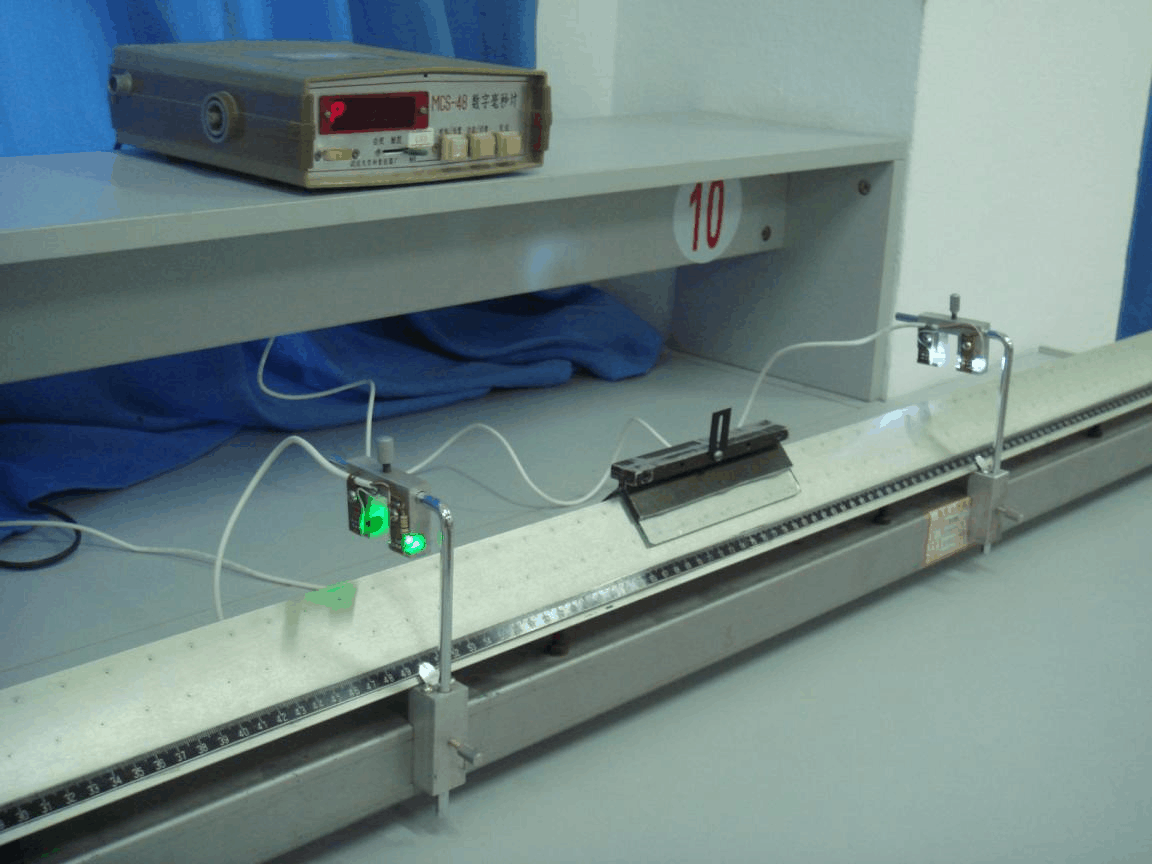
\includegraphics[width=0.6\textwidth]{figures/气垫导轨.png}
    \caption{气垫导轨装置}
    \label{fig:air_track}
\end{figure}

相比之下,本项目提出的基于YOLO AI视觉模型的测量方案具有显著优势:

\begin{enumerate}[leftmargin=*]
    \item 高精度数字化测量:模型可实时追踪摆球位置,精确记录完整运动轨迹,自动计算周期,消除人工计时误差;
    
    \item 低成本简易实现:仅需普通单摆装置和教学电脑即可完成,无需额外专业设备;
    
    \item 操作便捷友好:软件界面直观,学生只需拍摄视频并导入系统,即可获取完整数据集与分析结果;
    
    \item 物理原理可视化:系统自动生成位置-时间曲线,直观展示简谐运动特性,增强学生的物理概念理解。
    
\end{enumerate}

\subsection{阻尼系数测量的的教学创新应用}

在大学物理教学中,阻尼振动是重要的实验内容,但传统教学中学生对振动的位移-时间关系以及速度-时间关系缺乏感性认识。常见的沙摆留迹演示法存在如下明显缺陷:

\begin{enumerate}[leftmargin=*]
    \item 重心位置变化:随着沙的流出,沙漏的重心下降,导致单摆的摆长逐渐变长,周期随之变长,干扰了阻尼效应的观察;
    
    \item 匀速移动困难:实验中需用手牵动下方的纸板,很难保证运动匀速,导致生成的曲线不符合标准正弦衰减模型;
    
    \item 展示不便:实验得到的图形通常平铺在纸面上,不便立起或斜放给学生观察,限制了教学展示效果;
    
    \item 参数提取困难:从沙迹图像难以精确提取阻尼系数等关键参数,限制了定量分析。
\end{enumerate}

\begin{figure}[H]
    \centering
    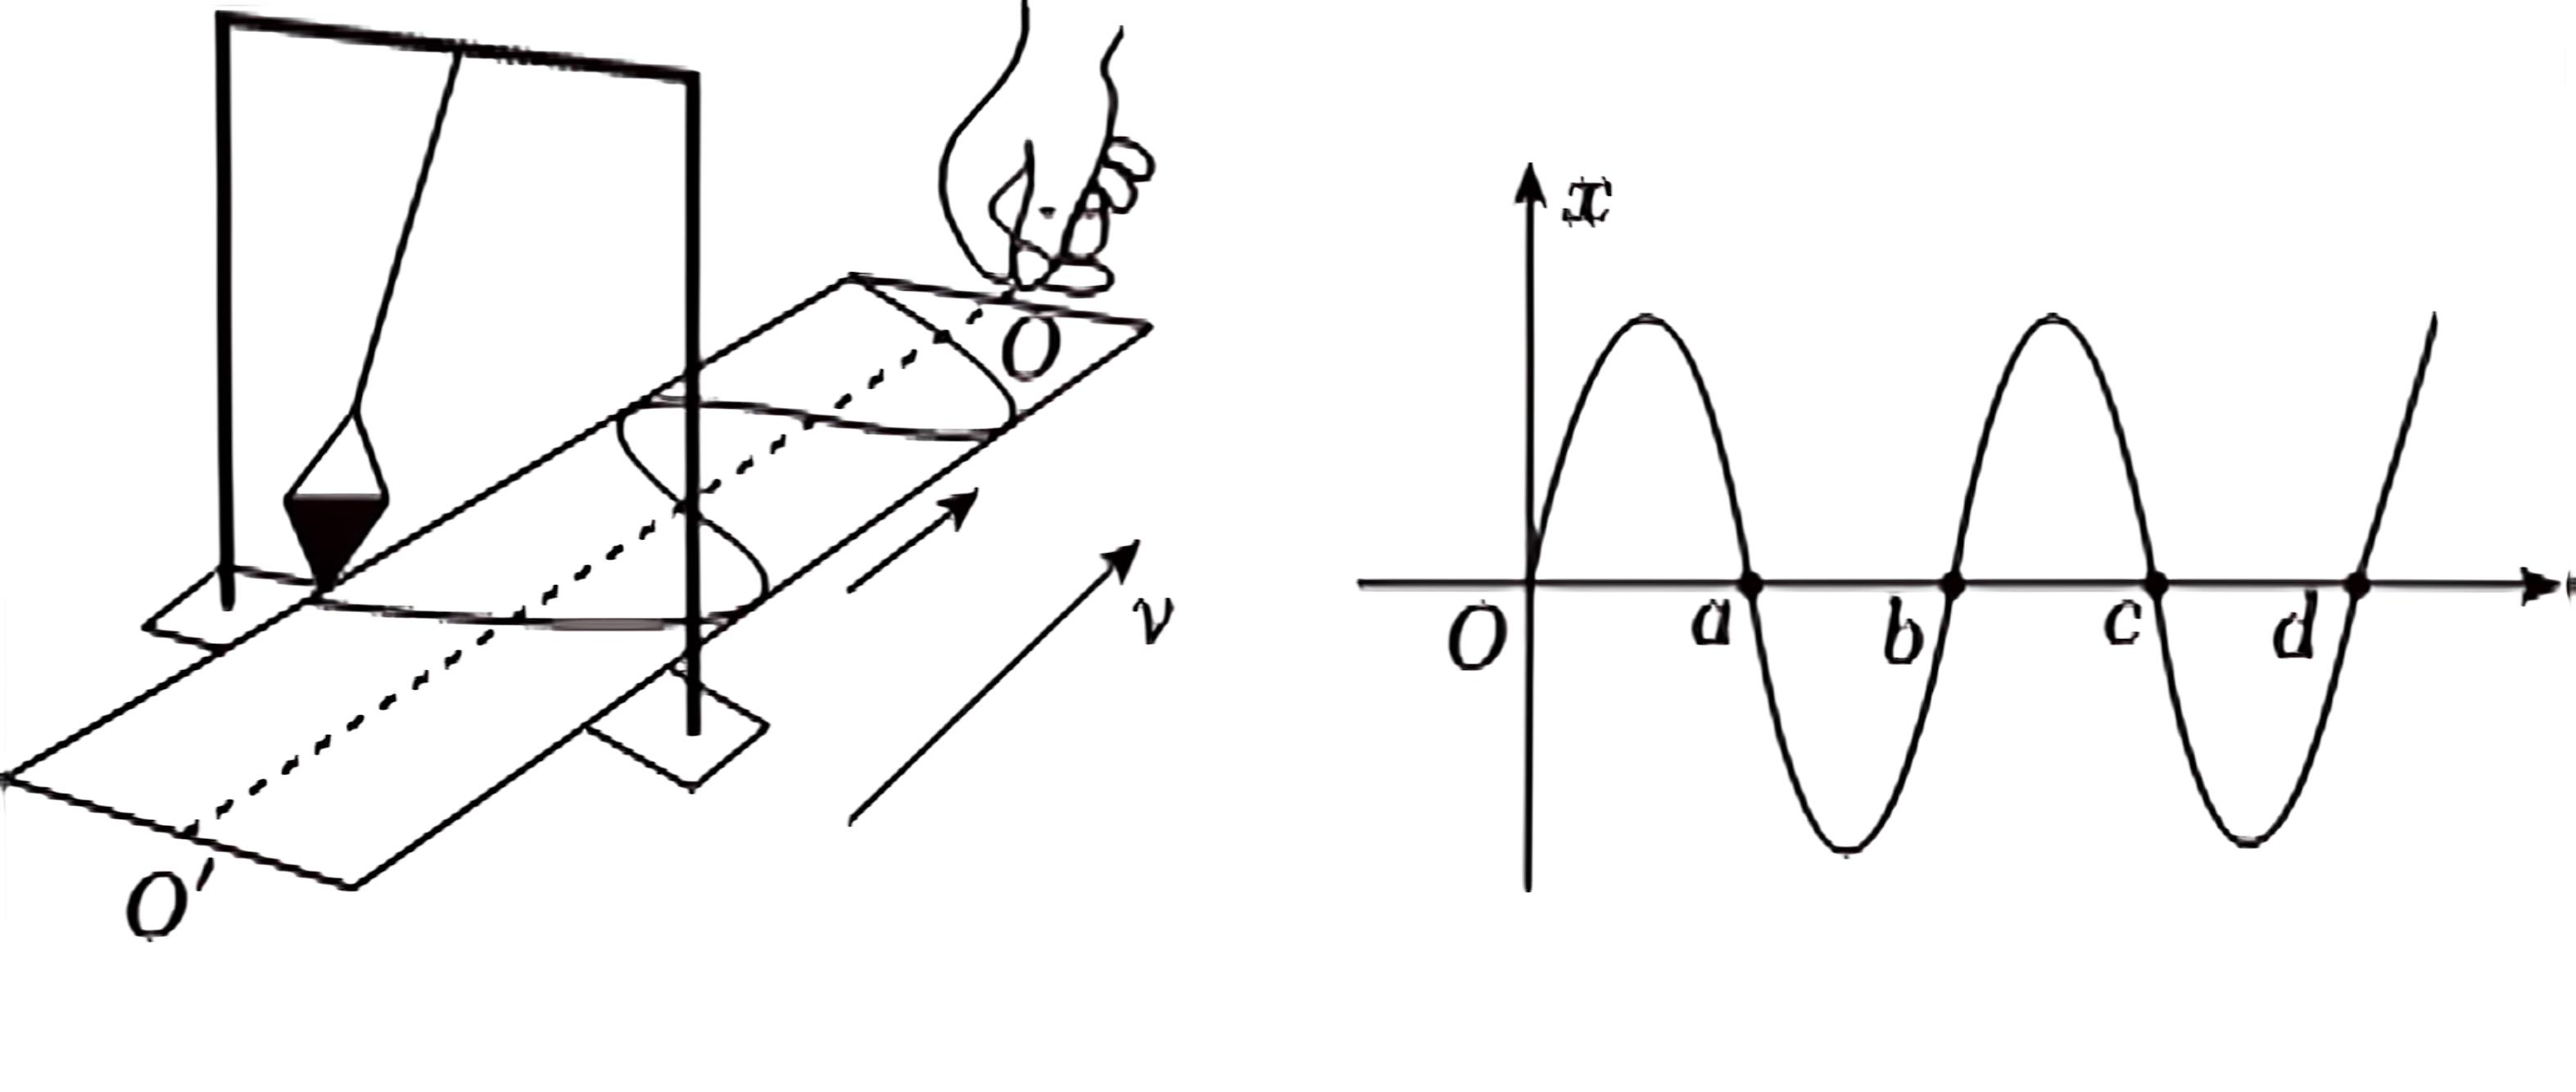
\includegraphics[width=0.6\textwidth]{figures/沙摆}
    \caption{沙摆实验示意图}
    \label{fig:sand_pendulum}
\end{figure}

本项目的AI辅助阻尼振动分析系统克服了上述缺点,为阻尼振动教学提供了全新解决方案:

\begin{enumerate}[leftmargin=*]
    \item 高精度轨迹追踪:系统可连续记录摆球位置,生成完整的位移-时间数据集,实现阻尼振动过程的精确量化;
    
    \item 多维度数据可视化:自动生成位置-时间曲线、速度-时间曲线、相位图和振幅衰减曲线,多角度展示阻尼振动特性;
    
    \item 参数自动计算:系统自动提取阻尼系数、固有频率、品质因数等关键参数,实现阻尼振动的定量分析;
    
    \item 交互式教学展示:通过软件界面可放大、缩小、暂停特定时间点的观察,或对比不同参数条件下的振动特性,增强教学交互性;
    
    \item 实验数据保存与共享:测量结果可导出为标准数据格式,便于学生课后分析或教师示范展示。
\end{enumerate}

在这些实验教学中,本团队探索将YOLO作为辅助教学工具,应用于单摆实验中。基于YOLO目标检测算法的教学软件能够实时、精准地捕捉摆球的位置信息,并自动生成运动数据文件。这些数据不仅为学生提供了更精确的实验数据,还帮助他们更直观地理解单摆的运动规律。学生可以利用这些数据通过软件绘制单摆的简谐运动图像、计算重力加速度和阻尼系数,这一创新使得学生能够更深入地理解阻尼运动的定量规律,将抽象的物理概念具象化,降低了实验操作难度,提高了实验的趣味性和教学效果。
\section{结论与展望}
\subsection{结论}

本项目基于YOLO深度学习目标检测算法,成功设计并实现了一套用于物理实验的智能自动化测量系统,实现了人工智能技术与传统物理实验的深度融合。通过系统实验与分析,本团队得出如下结论。

研究证明,\textbf{YOLO目标检测算法可以成功应用于物理实验中的动态目标追踪,实现对实验对象的精确定位与参数测量}。系统采用的三种互补周期测量方法(峰值检测法、FFT频谱分析法与曲线拟合法)结果高度一致,验证了系统的稳定性与可靠性。与传统人工测量方法相比,AI辅助测量显著提高了数据采集精度;与Tracker软件相比,本系统无需人工标定,并能在复杂背景下实现更高精度的测量。在重力加速度测量实验中,五组不同摆长的综合分析显示,最终测得的重力加速度平均值为$g = (9.785 \pm 0.319)$ m/s$^2$ (k=2),与武汉地区标准值$9.7936$ m/s$^2$相比,最佳测量结果的相对误差仅为0.02\%,\textbf{平均相对误差为0.19\%}。在阻尼系数测量方面,系统获得的本实验的阻尼系数为$(7.5 \pm 0.17) \times 10^{-5}$ N$\cdot$s/m (k=2),根据参考文献\textsuperscript{\cite{WUJS202211018}}理论分析,本实验测量结果与该单摆系统的实际阻尼系数相近。

不确定度分析表明,系统测量精度受到多种因素影响,主要包括:相机帧率限制导致的周期测量不确定度(贡献了重力加速度总不确定度的约99.1\%)以及YOLO目标检测的位置精度。重力加速度测量的合成相对不确定度为1.63\%,阻尼系数测量的合成相对不确定度为1.16\%,均显著优于传统手动测量方法。理论分析和实验结果均表明,当振幅比接近3.03时,阻尼系数的测量不确定度最小,这一发现为提高阻尼特性测量精度提供了重要指导。

系统实现了从视频数据采集到结果输出的全流程自动化处理,消除了人为操作误差,简化了实验步骤,显著提高了实验效率。系统基于普通单摆装置和常规摄像设备,无需额外专业仪器,大幅降低了实验成本,提高了技术推广的可行性。此外,图形化界面与数据可视化功能使物理过程直观呈现,有助于学生对周期运动和阻尼振动概念的理解,完成了AI技术与物理实验的有机结合。


\subsection{展望}

虽然本项目已取得初步成果,但在技术完善和应用拓展方面仍有广阔的发展空间。未来研究可从技术优化、应用拓展等方向展开深入探索。

在技术优化方面,本团队计划进一步扩充训练数据集规模,增强数据的多样性,引入更多光照条件、背景复杂度和摆球特征的变化,提升YOLO模型在复杂环境下的识别稳定性,同时探索模型轻量化方案,减少计算资源需求。本团队还将优化算法实现,提高视频处理和分析的实时性能,实现实验过程中的即时数据反馈,使系统不仅能用于事后分析,也能用于实时监测与教学演示。特别地,通过提高相机帧率至120 FPS,理论上可将重力加速度测量的总相对不确定度降低至约0.88\%,提升测量精度约46\%,这将是未来系统优化的重要方向。

在应用拓展方面,本系统可以适配到更多基础物理实验中,如自由落体、弹簧振子、碰撞实验、波动现象等,构建一个涵盖力学、电磁学、光学等领域的综合AI辅助实验平台,进一步探索AI实验平台与课程教学的融合。此外,基于本项目建立的不确定度评估体系,可以进一步完善物理实验中的测量精度分析方法,为学生提供更加全面的实验数据处理与误差分析训练。
\section{学生个人贡献}
本实验项目由来自数学与统计学院、物理与力学学院及信息学院的五位本科生组成的跨学科团队共同完成,在指导教师的悉心指导下,历时六个月完成了从系统构想到实验验证的完整研究流程。团队成员在人工智能、数据处理与物理实验等方面各有所长,形成了较为合理的知识结构与分工协作机制。

项目准备阶段(12 月至次年 1 月),团队对大学生物理实验竞赛的内容与评审标准进行了系统调研,明确了以“基于人工智能辅助的单摆周期测量系统”为研究主题。通过查阅相关文献与技术资料,确定采用基于 YOLO 模型的目标检测算法结合图像分析手段进行周期自动提取的可行技术路线。

项目初期(2 月至 3 月),团队完成了初代实验平台的搭建,实现了高质量视频采集、YOLO 模型的部署与测试,并构建了像素级运动轨迹提取模块,初步验证了图像识别在摆运动测量中的有效性。

项目中期(3 月至 4 月),着重开发了数据处理与周期分析模块,涵盖信号平滑、峰值检测、周期计算与拟合分析等关键算法,实现了系统对实验数据的自动分析处理。期间团队同步进行多组物理场景实验拍摄与数据测试,反复调试以提升系统鲁棒性与分析精度。

项目末期(4 月至 5 月),团队在前期工作的基础上对各模块功能进行了集成与优化,确保系统运行稳定、输出准确。同时,完成了实验报告的撰写与 LaTeX 文档排版,制作了完整的系统演示视频,最终形成了具备展示性、实用性与创新性的竞赛项目成果。

\begin{table}[H]
\centering
\caption{学生个人贡献表}
\begin{tabular}{@{}c p{12.5cm}@{}}
\toprule
\textbf{队员编号} & \multicolumn{1}{c}{\textbf{个人贡献}} \\
\midrule
1 & 项目负责人,负责整体统筹与任务分配,设计AI辅助实验系统方案。主要负责YOLO模型的训练与数据预处理,包括图像标注、模型调参与结果验证,并撰写关键技术文档与实验报告。 \\
2 & 主要负责论文撰写与排版,整理技术内容并规范表达,协调各模块内容整合为完整文本,同时美化数据图表,确保论文质量与表达规范。 \\
3 & 协助完成YOLO模型训练、部署与输出数据处理,参与图像标注与周期提取精度分析,后期协助视频拍摄与剪辑,提升项目展示效果。 \\
4 & 负责实验平台搭建与调试,包括摆锤结构设计、视频采集设置及相机校准,保障数据采集稳定性,同时参与PPT制作与展示材料整理。 \\
5 & 负责数据处理模块开发,实现周期提取相关算法,并与YOLO输出有效对接,提升系统自动化水平,协助论文代码内容的逻辑校对与验证。 \\
\bottomrule
\end{tabular}
\label{tab:contribution}
\end{table}

\nocite{*}
\printbibliography[heading=bibintoc, title=\ebibname]

\appendix
\appendixpage
\addappheadtotoc

\section{实验数据}
\subsection{原始数据}

\subsubsection{重力加速度测量结果}
\begin{table}[H]
\centering
\threelinetablestyle
\caption{重力加速度测量结果}
\setlength{\tabcolsep}{3pt}
\footnotesize
\begin{tabular}{cclcccccccc}
\toprule
编号 & 测量摆长 & 使用的 & 最大 & 大摆角 & FFT周期 & FFT重力 & FFT误差 & Peak周期 & Peak重力 & Peak误差 \\
 & (m) & 测量方法 & 角(°) & 修正 & (s) & (m/s²) & (\%) & (s) & (m/s²) & (\%) \\
\midrule
1 & 0.3505 & FFT, Peak & 5 & 1.000 & 1.191 & 9.738 & 0.57 & 1.192±0.008 & 9.718 & 0.77 \\
2 & 0.3501 & FFT, Peak, Fit & 5 & 1.000 & 1.189 & 9.772 & 0.22 & 1.192±0.007 & 9.731 & 0.64 \\
3 & 0.3499 & FFT, Peak & 5 & 1.000 & 1.187 & 9.806 & 0.13 & 1.192±0.008 & 9.720 & 0.75 \\
4 & 0.3495 & FFT, Peak & 5 & 1.000 & 1.190 & 9.758 & 0.36 & 1.189±0.008 & 9.773 & 0.21 \\
5 & 0.3500 & FFT, Peak, Fit & 5 & 1.000 & 1.184 & 9.849 & 0.56 & 1.190±0.008 & 9.758 & 0.36 \\
\bottomrule
\end{tabular}
\label{tab:gravity_measurement}
\end{table}
\label{app:gravity_measurement}

\subsubsection{摆长与周期的关系}
\begin{table}[H]
\centering
\threelinetablestyle
\caption{摆长与周期的关系(钢小球)(标准重力加速度值:9.7936 m/s²)}
\setlength{\tabcolsep}{2pt}
\footnotesize
\begin{tabular}{cccccccccccc}
\toprule
摆长 & 最大 & 测量 & 未修正 & 未修正 & 未修正 & 大摆角 & 修正后 & 修正后 & 最终采用 & 最终重力 & 最终 \\
(m) & 摆角(°) & 方法 & 周期(s) & 重力加速度 & 相对误差 & 修正系数 & 重力加速度 & 相对误差 & 方法 & 加速度 & 相对误差 \\
 & & & & (m/s²) & (\%) & & (m/s²) & (\%) & & (m/s²) & (\%) \\
\midrule
0.33 & 5 & FFT & 1.156 & 9.745 & 0.5 & 1.000476 & 9.754 & 0.4 & Peak & 9.774 & 0.2 \\
0.33 & 5 & Peak & 1.155 $\pm$ 0.008 & 9.765 & 0.29 & 1.000476 & 9.774 & 0.2 & Peak & 9.774 & 0.2 \\
0.33 & 5 & Fit & 1.156 & 9.755 & 0.39 & 1.000476 & 9.765 & 0.3 & Peak & 9.774 & 0.2 \\
0.34 & 5 & FFT & 1.174 & 9.737 & 0.58 & 1.000476 & 9.746 & 0.49 & Fit & 9.747 & 0.47 \\
0.34 & 5 & Peak & 1.175 $\pm$ 0.014 & 9.722 & 0.73 & 1.000476 & 9.731 & 0.63 & Fit & 9.747 & 0.47 \\
0.34 & 5 & Fit & 1.174 & 9.738 & 0.57 & 1.000476 & 9.747 & 0.47 & Fit & 9.747 & 0.47 \\
0.35 & 5 & FFT & 1.193 & 9.715 & 0.8 & 1.000476 & 9.724 & 0.71 & Fit & 9.725 & 0.7 \\
0.35 & 5 & Peak & 1.193 $\pm$ 0.008 & 9.711 & 0.85 & 1.000476 & 9.72 & 0.75 & Fit & 9.725 & 0.7 \\
0.35 & 5 & Fit & 1.193 & 9.716 & 0.79 & 1.000476 & 9.725 & 0.7 & Fit & 9.725 & 0.7 \\
0.36 & 5 & FFT & 1.195 & 9.96 & 1.7 & 1.000476 & 9.969 & 1.79 & Fit & 9.725 & 0.7 \\
0.36 & 5 & Peak & 1.210 $\pm$ 0.008 & 9.7 & 0.95 & 1.000476 & 9.71 & 0.86 & Fit & 9.725 & 0.7 \\
0.36 & 5 & Fit & 1.209 & 9.716 & 0.8 & 1.000476 & 9.725 & 0.7 & Fit & 9.725 & 0.7 \\
0.37 & 5 & FFT & 1.228 & 9.684 & 1.12 & 1.000476 & 9.693 & 1.03 & Fit & 9.765 & 0.29 \\
0.37 & 5 & Peak & 1.225 $\pm$ 0.008 & 9.734 & 0.61 & 1.000476 & 9.743 & 0.51 & Fit & 9.765 & 0.29 \\
0.37 & 5 & Fit & 1.224 & 9.756 & 0.38 & 1.000476 & 9.765 & 0.29 & Fit & 9.765 & 0.29 \\
\bottomrule
\end{tabular}
\label{tab:length_and_period}
\end{table}
\label{app:length_and_period}

\subsubsection{大摆角的非线性修正效果}
\begin{table}[H]
\centering
\threelinetablestyle
\caption{大摆角的非线性修正效果(钢小球)(标准重力加速度值:9.7936 m/s²)}
\setlength{\tabcolsep}{2pt}
\footnotesize
\begin{tabular}{cccccccccccc}
\toprule
摆长 & 最大 & 测量 & 未修正 & 未修正 & 未修正 & 大摆角 & 修正后 & 修正后 & 最终采用 & 最终重力 & 最终 \\
(m) & 摆角(°) & 方法 & 周期(s) & 重力加速度 & 相对误差 & 修正系数 & 重力加速度 & 相对误差 & 方法 & 加速度 & 相对误差 \\
 & & & & (m/s²) & (\%) & & (m/s²) & (\%) & & (m/s²) & (\%) \\
\midrule
0.35 & 5 & FFT & 1.193 & 9.715 & 0.8 & 1.000476 & 9.724 & 0.71 & Fit & 9.725 & 0.7 \\
0.35 & 5 & Peak & 1.193 $\pm$ 0.008 & 9.711 & 0.85 & 1.000476 & 9.72 & 0.75 & Fit & 9.725 & 0.7 \\
0.35 & 5 & Fit & 1.193 & 9.716 & 0.79 & 1.000476 & 9.725 & 0.7 & Fit & 9.725 & 0.7 \\
0.35 & 10 & FFT & 1.19 & 9.758 & 0.36 & 1.001907 & 9.795 & 0.02 & FFT & 9.795 & 0.02 \\
0.35 & 10 & Peak & 1.185 $\pm$ 0.045 & 9.832 & 0.39 & 1.001907 & 9.869 & 0.77 & FFT & 9.795 & 0.02 \\
0.35 & 10 & Fit & 1.184 & 9.858 & 0.65 & 1.001907 & 9.895 & 1.04 & FFT & 9.795 & 0.02 \\
0.35 & 15 & FFT & 1.183 & 9.878 & 0.87 & 1.004301 & 9.964 & 1.74 & Peak & 9.835 & 0.43 \\
0.35 & 15 & Peak & 1.190 $\pm$ 0.040 & 9.751 & 0.43 & 1.004301 & 9.835 & 0.43 & Peak & 9.835 & 0.43 \\
0.35 & 15 & Fit & 1.188 & 9.786 & 0.08 & 1.004301 & 9.87 & 0.78 & Peak & 9.835 & 0.43 \\
0.35 & 20 & FFT & 1.19 & 9.764 & 0.3 & 1.007669 & 9.914 & 1.23 & Peak & 9.828 & 0.35 \\
0.35 & 20 & Peak & 1.195 $\pm$ 0.047 & 9.679 & 1.17 & 1.007669 & 9.828 & 0.35 & Peak & 9.828 & 0.35 \\
0.35 & 20 & Fit & 1.19 & 9.763 & 0.31 & 1.007669 & 9.913 & 1.22 & Peak & 9.828 & 0.35 \\
0.35 & 25 & FFT & 1.215 & 9.358 & 4.45 & 1.012029 & 9.584 & 2.14 & Fit & 9.837 & 0.44 \\
0.35 & 25 & Peak & 1.195 $\pm$ 0.031 & 9.672 & 1.25 & 1.012029 & 9.906 & 1.14 & Fit & 9.837 & 0.44 \\
0.35 & 25 & Fit & 1.199 & 9.604 & 1.93 & 1.012029 & 9.837 & 0.44 & Fit & 9.837 & 0.44 \\
\bottomrule
\end{tabular}
\label{tab:large_angle_correction}
\end{table}
\label{app:large_angle_correction}

\subsubsection{阻尼特性测量结果}
\begin{table}[H]
\centering
\threelinetablestyle
\caption{阻尼特性测量结果(塑料小球)}
\setlength{\tabcolsep}{2pt}
\footnotesize
\begin{tabular}{cccccccccccc}
\toprule
摆长 & 最大 & 摆球质量 & 初始 & n个周期后 & 周期数 & 周期 & 阻尼系数 & 衰减系数 & 固有频率 & 品质因数 & 衰减时间 \\
(m) & 摆角(°) & (kg) & 振幅 $\theta_0$ & 振幅 $\theta'$ & n & T (s) & $\beta$ (N·s/m) & $\gamma$ (s$^{-1}$) & $\omega_0$ (rad/s) & Q & 常数 $\tau$ (s) \\
\midrule
0.8 & 5 & 0.004 & 349.46 & 115.53 & 33 & 1.788 & 0.000075 & 0.018762 & 3.5149 & 93.67 & 53.3 \\
0.8 & 5 & 0.004 & 344.5 & 114.35 & 33 & 1.788 & 0.000075 & 0.018694 & 3.5148 & 94.01 & 53.49 \\
0.8 & 5 & 0.004 & 347.64 & 115.01 & 33 & 1.789 & 0.000075 & 0.018735 & 3.5119 & 93.72 & 53.37 \\
0.8 & 5 & 0.004 & 345.5 & 113.87 & 33 & 1.787 & 0.000075 & 0.01882 & 3.5158 & 93.41 & 53.13 \\
0.8 & 5 & 0.004 & 349.34 & 112.48 & 33 & 1.788 & 0.000077 & 0.01921 & 3.5148 & 91.49 & 52.06 \\
\bottomrule
\end{tabular}
\label{tab:damping_measurement}
\end{table}
\label{app:damping_measurement}

\subsubsection{摆长对阻尼特性的影响}
\begin{table}[H]
\centering
\threelinetablestyle
\caption{摆长对阻尼特性的影响}
\setlength{\tabcolsep}{2pt}
\footnotesize
\begin{tabular}{cccccccccccc}
\toprule
摆长 & 最大 & 摆球质量 & 初始 & n个周期后 & 周期数 & 周期 & 阻尼系数 & 衰减系数 & 固有频率 & 品质因数 & 衰减时间 \\
(m) & 摆角(°) & (kg) & 振幅 $\theta_0$ & 振幅 $\theta'$ & n & T (s) & $\beta$ (N·s/m) & $\gamma$ (s$^{-1}$) & $\omega_0$ (rad/s) & Q & 常数 $\tau$ (s) \\
\midrule
0.4 & 5 & 0.009 & 233.59 & 197.34 & 13 & 1.278 & 0.000091 & 0.010147 & 4.9156 & 484.46 & 98.55 \\
0.55 & 5 & 0.009 & 388.55 & 311.66 & 13 & 1.496 & 0.000102 & 0.011336 & 4.1996 & 370.46 & 88.21 \\
0.7 & 5 & 0.009 & 465.3 & 397.97 & 8 & 1.683 & 0.000104 & 0.011606 & 3.7326 & 321.60 & 86.16 \\
0.85 & 5 & 0.009 & 504.49 & 403.96 & 10 & 1.855 & 0.000108 & 0.011979 & 3.3872 & 282.76 & 83.48 \\
1 & 5 & 0.009 & 529.58 & 428.9 & 8 & 2.004 & 0.000118 & 0.013151 & 3.135 & 238.38 & 76.04 \\
\bottomrule
\end{tabular}
\label{tab:length_effect_on_damping}
\end{table}

\subsubsection{尺寸对阻尼特性的影响}
\begin{table}[H]
\centering
\threelinetablestyle
\caption{尺寸对阻尼特性的影响}
\setlength{\tabcolsep}{2pt}
\footnotesize
\begin{tabular}{ccccccccccc}
\toprule
\multicolumn{11}{c}{塑料小球} \\
\midrule
摆长 & 最大 & 摆球质量 & 初始 & n个周期后 & 周期数 & 周期 & 阻尼系数 & 衰减系数 & 固有频率 & 衰减时间 \\
(m) & 摆角(°) & (kg) & 振幅 $\theta_0$ & 振幅 $\theta'$ & n & T (s) & $\beta$ (N·s/m) & $\gamma$ (s$^{-1}$) & $\omega_0$ (rad/s) & $\tau$ (s) \\
\midrule
0.8 & 5 & 0.004 & 396.38 & 257.35 & 11 & 1.785 & 0.000088 & 0.022001 & 3.5203 & 45.45 \\
0.8 & 5 & 0.004 & 399.69 & 266.9 & 10 & 1.785 & 0.00009 & 0.022622 & 3.52 & 44.21 \\
0.8 & 5 & 0.004 & 396.81 & 256.31 & 11 & 1.785 & 0.000089 & 0.022263 & 3.5203 & 44.92 \\
\midrule
\multicolumn{11}{c}{塑料大球} \\
\midrule
0.8 & 5 & 0.009 & 363.11 & 296.93 & 10 & 1.777 & 0.000102 & 0.011324 & 3.5365 & 88.31 \\
0.8 & 5 & 0.009 & 371.4 & 304.25 & 10 & 1.778 & 0.000101 & 0.011215 & 3.5332 & 89.17 \\
0.8 & 5 & 0.009 & 351.34 & 266.38 & 13 & 1.777 & 0.000108 & 0.011984 & 3.536 & 83.45 \\
\bottomrule
\end{tabular}
\label{tab:size_effect_on_damping}
\end{table}
\label{app:size_effect_on_damping}

\subsubsection{质量对阻尼特性的影响}
\begin{table}[H]
\centering
\threelinetablestyle
\caption{质量对阻尼特性的影响}
\setlength{\tabcolsep}{2pt}
\footnotesize
\begin{tabular}{ccccccccccc}
\toprule
\multicolumn{11}{c}{不锈钢小球0.8m摆长5度} \\
\midrule
编号 & 摆球质量 & 初始振幅 & n个周期后 & 周期数 & 周期 & 阻尼系数 & 衰减系数 & 固有频率 & 品质因数 & 衰减时间 \\
 & (kg) & $\theta_0$ & 振幅 $\theta'$ & n & T (s) & $\beta$ (N·s/m) & $\gamma$ (s$^{-1}$) & $\omega_0$ (rad/s) & Q & $\tau$ (s) \\
\midrule
1 & 0.031 & 462.44 & 429.37 & 11 & 1.798 & 0.000116 & 0.00375 & 3.4936 & 931.68 & 266.68 \\
2 & 0.031 & 479.24 & 445.9 & 11 & 1.798 & 0.000113 & 0.003645 & 3.4936 & 958.42 & 274.34 \\
3 & 0.031 & 464.74 & 431.59 & 11 & 1.797 & 0.000116 & 0.003743 & 3.4965 & 934.10 & 267.15 \\
\midrule
\multicolumn{11}{c}{塑料小球0.8m摆长5度} \\
\midrule
1 & 0.004 & 396.38 & 257.35 & 11 & 1.785 & 0.000088 & 0.022001 & 3.5203 & 160.00 & 45.45 \\
2 & 0.004 & 399.69 & 266.9 & 10 & 1.785 & 0.00009 & 0.022622 & 3.52 & 155.60 & 44.21 \\
3 & 0.004 & 396.81 & 256.31 & 11 & 1.785 & 0.000089 & 0.022263 & 3.5203 & 158.12 & 44.92 \\
\bottomrule
\end{tabular}
\label{tab:mass_effect_on_damping}
\end{table}
\label{app:mass_effect_on_damping}

\section{软件代码}
\label{app:software_code}
\subsection{视频处理代码}
\lstinputlisting[language=Python, caption=视频处理代码, label=code:video_processing]{code/tracker.py}
\subsection{数据分析代码}
\lstinputlisting[language=Python, caption=数据分析代码, label=code:data_analysis]{code/analyzer.py}
\subsection{GUI代码}
非核心功能代码,用于构建软件交互界面,篇幅过长,不作展示。

\end{document}